\documentclass[12pt,a4paper]{report}
% !TEX TS-program = xelatex

%%Global shortcuts/variables
\def\ehw{\textbf{EHW}}
\def\randr{\textit{\textbf{Rules \& Regulations}}}

%%Template provided by EHW. Tachyon Hyperloop added minor changes.
%%%%%%%% CREATE DOCUMENT STRUCTURE %%%%%%%%
%% Language and font encodings
\usepackage[english]{babel}
\usepackage[utf8x]{inputenc}
\usepackage[T1]{fontenc}
%\usepackage{subfig}

%% Sets page size and margins
\usepackage[a4paper,top=2cm,bottom=2cm,left=2cm,right=2cm,marginparwidth=2cm]{geometry}


% Packages 
\usepackage{graphicx} % To include images
\usepackage[colorlinks=true, allcolors=blue]{hyperref} % For hyperlinks
\usepackage{amsmath}  % For mathematical expressions
\usepackage{amsfonts} % For mathematical fonts
\usepackage{tikz} % for diagrams
\usetikzlibrary{positioning, circuits.ee.IEC}


\usepackage{comment}
\usepackage{verbatim}
\usepackage{sectsty}
\usepackage{float}
\usepackage{titling} 
\usepackage{blindtext}
\usepackage[square,sort,comma,numbers]{natbib}
\usepackage[colorinlistoftodos]{todonotes}
\usepackage{xcolor}
\usepackage[shortlabels]{enumitem}
\usepackage{tabularray}
\usepackage{textcomp, gensymb}
\usepackage{wallpaper}
%\usepackage{background}
\usepackage{afterpage}
\definecolor{ehwBlue}{rgb}{0, 0, 0.741}
\definecolor{ehwOrange}{rgb}{0.839,0.8117,0.72156}
\usepackage{titlesec}
\usepackage{colortbl}
\usepackage{fontspec}

\usepackage{wrapfig}
\usepackage{forloop}
\usepackage{mfirstuc}
\usepackage{longtable}
\usepackage{adjustbox}
\usepackage{multirow}
\usepackage{eurosym}
\usepackage[nameinlink]{cleveref}
\usepackage{subcaption}
\usepackage{caption}
\usepackage{booktabs}



%This limits the depth of table of contents to 2 step until sections
\setcounter{tocdepth}{1}

\titleformat{\chapter} % Changes the font  color for all chapter titles
{\color{ehwBlue}\normalfont\Large\bfseries}
{\thesection}
{1em}
{}
\titleformat{\section} % Changes the font  color for all section titles
{\color{ehwBlue}\normalfont\large\bfseries}
{\thesection}
{1em}
{}
\titleformat{\subsection}% Changes the font  color for all subsection titles
{\color{ehwBlue}\normalfont\normalsize\bfseries}
{\thesubsection}
{1em}
{}
\titleformat{\subsubsection}% Changes the font  color for all subsubsection titles
{\color{ehwBlue}\normalfont\normalsize\bfseries}
{\thesubsubsection}
{1em}
{}

\arrayrulecolor{ehwBlue} % This changes the color of all tables to EHW blue

\begin{comment}
  

\setmainfont{Regular.ttf} % Sets the font of the document to regular Breite Grotesk
% 
\newfontfamily\headingfont[]{Light.ttf} % Changes the type of font for the headers
\titleformat*{\section}{\Large\color{ehwBlue}{\headingfont}}
\titleformat*{\subsection}{\large\color{ehwBlue}{\headingfont}}
\titleformat*{\subsubsection}{\large\color{ehwBlue}{\headingfont}}
\end{comment}


\setlength{\headheight}{2pt}

\renewcommand{\labelitemi}{\textcolor{ehwBlue}{$\bullet$}} % There was a mistake with itemize list. So this fixes it by making all the points bullets.


%%%Optional. \iffalse if otherwise.
\iffalse
\fancypagestyle{mypagestyle}{%
  \fancyhf{}% Clear header/footer
  \fancyhead[OC]{\textcolor{ehwBlue}{European Hyperloop Week}}% Author on Odd page, Centred
  \fancyhead[EC]{\textcolor{ehwBlue}{Rules \& Regulations}}% Title on Even page, Centred
  \fancyfoot[C]{\thepage}%
  \renewcommand{\headrulewidth}{.4pt}% Header rule of .4pt
  \renewcommand{\headrule}{\color{ehwBlue}\hrule}
  \fancyfoot[C]{\color{ehwBlue}{\textbf{\thepage}}}
} % This creates a new type of page setup, where the odd pages are marked with European Hyperloop week and the even pages say the name of the document

\fancypagestyle{nobgpagestyle}{
  \fancyhf{}% Clear header/footer
  % Define any other formatting for the blank pages here
}
\fi




\setlength{\footskip}{25pt} % With this I changed the position of the page numbers so that it fits into the image

\newfontfamily\italicfont{Light Condensed.ttf} % Sets the italics font to Condensed Breite Grotesk. I couldn't make it work by normal means since the ttf package apparently doesn't contain information regarding how the font will look in italics or bold.

%\newgeometry{top=1in, bottom=1in, left=1in, right=1in}

\setlength\extrarowheight{4.5pt} % This increases the size of the cells so the text seems to fit better.

% This is to create an intentionally left-blank page
\newcommand{\blankpage}{
  \thispagestyle{nobgpagestyle}
  \begin{center}
    \vspace*{\fill}
    This page has been left intentionally blank.
    \vspace*{\fill}
  \end{center}
  \newpage
}

% Redefine the appearance of the checkbox
% Define a counter for the checkboxes
\newcounter{checkboxcount}
\setcounter{checkboxcount}{0}

% Define the checkbox style with blue border
\newcommand{\bluecheckbox}{%
  \stepcounter{checkboxcount}%
  \textcolor{ehwBlue}{\CheckBox[height=0.4cm, width=0.4cm, name=task\thecheckboxcount]{}}
}



% Remove "Chapter" prefix from chapter titles
\titleformat{\chapter}[display]
  {\normalfont\huge\bfseries}{}{0pt}{\LARGE}


\begin{document}
%Created by ChatGPT 4, courtesy of Pascal.


% Since \include forces a new page, use it thoughtfully
% Cover Page
% Note: With \include, make sure to not include file extension
\begin{titlepage}
    \newcommand{\HRule}{\rule{\linewidth}{0.5mm}}
    % horizontal line and its thickness
    \center 
     
    % University
    
\includegraphics[width=0.2\textwidth]{backgroundimages/ZurichImage.png}\\[1cm]
    
    % Document info
                                    % Course Code
    {\color{ehwBlue}\HRule} \\[0.8cm]
    {\fontsize{36}{42}\selectfont \bfseries \textcolor{ehwBlue}{{FDD}}}\\[0.7cm]		% Assignment
    {\color{ehwBlue}\HRule} \\[2cm]
    \textsc{\LARGE\textcolor{ehwBlue}{ European Hyperloop Week}}\\[1cm]
    \large
    
    
    \textcolor{ehwBlue}{Tachyon Hyperloop}\\[1.5cm]
    \huge \textcolor{ehwBlue}{March 17, 2024}\\[4cm]
    
\includegraphics[width=0.3\textwidth]{backgroundimages/LogoBlue.png}\\[1cm] 	% University logo
    \vfill 
    \ThisLRCornerWallPaper{1}{backgroundimages/BackgroundCover.png}
\end{titlepage}
    % \begin{center}
    %     \makebox[\textwidth]{ \includegraphics[width=\paperwidth]{backgroundimages/image9.png}}
    % \end{center}
    
% If the Tachyon cover page is for a different section/part, include it where appropriate
%\include{/texfiles/general/coverpageTachyon}

% Table of Contents
\tableofcontents


% Introduction
\chapter{Introduction}

Tachyon Hyperloop e.V. is a pioneering initiative conceived in 2019 by students from RWTH Aachen University and FH Aachen University of Applied Sciences. Inspired by Elon Musk's groundbreaking vision of the Hyperloop in 2013, our team comprises 35 dedicated students from diverse academic backgrounds, all unified by our shared commitment to pushing the boundaries of knowledge and technology within the transportation sector.

Our team functions seamlessly across six specialized departments: Mechanical, Electrical, Project Management, Business and Marketing, Sponsoring, and Architecture \& Urban Design. Each department is led by a proficient team lead, ensuring clear communication and effective coordination across all project facets. Guided by the strategic oversight of board members including Jacob Diercks, Marijan Schlösser, and Yashasvi Karnena, we navigate the complex landscape of Hyperloop innovation with determination and vision.
\section{FDD.7 Applicant and List of Team Members}
\begin{table}[h]
\centering
\begin{tabular}{|l|l|}
\hline
\textbf{Name}           & \textbf{Department}        \\ \hline
Jacob Dierck            & First Chairman             \\ \hline
Marijan Schlösser       & Second Chairman            \\ \hline
Yashasvi Karnena        & Treasurer                  \\ \hline
Pascal Pfeifer          & Mechanical Department      \\ \hline
Lennart Jepsen          & Mechanical Department      \\ \hline
Niclas Vermeulen        & Mechanical Department      \\ \hline
Shreepad Khedkar        & Mechanical Department      \\ \hline
Benjamin Köhler         & Mechanical Department      \\ \hline
Jasmin Dedeoglu         & Mechanical Department      \\ \hline
Aniket Saxena           & Mechanical Department      \\ \hline
Kanishk Singh           & Mechanical Department      \\ \hline
Yash Shah               & Mechanical Department      \\ \hline
Rengin Solmaz           & Mechanical Department      \\ \hline
Sachin Salaskar         & Mechanical Department      \\ \hline
Guru Bysani             & Mechanical Department      \\ \hline
Aryan Modi              & Mechanical Department      \\ \hline
Vaishnavi Ramkumar      & Mechanical Department      \\ \hline
Dino Cheng              & Electrical Department      \\ \hline
Abhishek Jha            & Electrical Department      \\ \hline
Sourajit Majumder       & Electrical Department      \\ \hline
Stefan Boskovic         & Electrical Department      \\ \hline
Bohdan Popov            & Electrical Department      \\ \hline
Ian Morales             & Electrical Department      \\ \hline
Paula Vicente           & Electrical Department      \\ \hline
Aryan Kumalajati        & Electrical Department      \\ \hline
Praneet Tuli            & Project Management         \\ \hline
Duc Thiem Do            & Project Management         \\ \hline
Till Behringer          & Project Management         \\ \hline
Ludwig Gatzsch          & Business \& Marketing      \\ \hline
Henriette Brucks        & Business \& Marketing      \\ \hline
Joana Baumann           & Sponsoring                 \\ \hline
Carl-Philipp Schetelig  & Sponsoring                 \\ \hline
Clara Kamrath           & Architecture \& Urban Design \\ \hline
Hannes Wittkopf         & Architecture \& Urban Design \\ \hline
Janik Hiob              & Architecture \& Urban Design \\ \hline
\end{tabular}
\caption{Team Members and Departments}
\label{tab:team}
\end{table}

\section{FDD.8 Development Environment and Research Objectives}
Despite the demands of our academic pursuits, we dedicate ourselves fully to the Tachyon initiative. From our inception, we have found a home at the Collective Incubator, a vibrant hub that fosters collaboration and innovation. Previously, we benefited from the facilities at the WZL, an institute of RWTH Aachen University, before transitioning to our current workspace. This dynamic environment has nurtured our growth and facilitated the realization of our ambitious projects.

Our endeavors are sustained through a blend of financial support from sponsors, generous donations, and contributions from supporting organizations. Tachyon Hyperloop epitomizes our collective aspiration to design and construct functional prototypes of Hyperloop Pods, contributing significantly to the advancement of transportation technology on a global scale.

Acknowledging our sponsors is pivotal to the success of our projects. We extend our heartfelt appreciation to RWTH Aachen University for their unwavering support throughout our journey. Special gratitude is also extended to Institut für Allgemeine Mechanik for their invaluable expertise and infrastructure. Additionally, we express our gratitude to proRWTH, WZL, and International Academy for their unwavering support. We extend our heartfelt thanks to EVS Euregio GmbH for providing a testing track and to Collective Incubator e.V. for their provision of an exceptional office space. Special thanks are extended to our sponsor-partners STAWAG, Emrax, Mouser, Contitech AG, Leaddrive, Vector, PWC and Dürr  for their substantial material and financial support. Finally, we would like to express our appreciation to the European Hyperloop Week Committee for providing us with the opportunity to showcase our project, facilitating collaboration, information sharing, and networking within the Hyperloop community.

Apart from our primary projects highlighted in this documentation, Tachyon Hyperloop e.V. is also engaged in other initiatives that are integral to our research and development.

One such project is Pathfinder. As one of the few teams to have our own test track near Aachen, generously provided by our partner EVS EUREGIO Verkehrsschienennetz GmbH, our 1 km long test track stands as one of the longest among student teams. For the upcoming European Hyperloop Week 2024 competition, we have collaborated with Swissloop to utilize their track infrastructure. This partnership aims to foster knowledge exchange, allowing us to gain valuable insights into the limitations and advantages of their track design. By sharing the same tracks, we also anticipate significant cost efficiencies. The strategic collaboration between our teams promises mutual benefits, facilitating innovation and advancement within the Hyperloop community.

Additionally, the Minipod project plays a vital role in our development process. Serving as a prototype of the prototype, the Minipod enables us to mitigate risks associated with resource allocation and system functionality before implementing them on a larger scale. By developing and testing on a smaller scale, we can gather valuable insights and refine our technologies with reduced risk.

In the upcoming sections, we will delve into a comprehensive System Overview, offering a succinct understanding of the Pod. Following this, we will explore the Mechanical system, intricately detailing the design and construction of our pod. Our focus will then shift to the Electrical domain, where we will discuss vital components such as the Sense \& Control systems crucial for our pod's functionality. Additionally, we will address Safety measures implemented to ensure the well-being of our team and the success of of our project. Through these sections, our aim is to provide a detailed insight into our project's development process, while adhering to the guidelines and regulations outlined by the European Hyperloop Week Committee.

\section{FDD.10 Category for This Application}

% Mechanical Systems
\chapter{Mechanical Systems}

\section{Introduction}
% Mechanical introduction content here



\section{Chassis}




\subsection{Overview}


\subsubsection{Requirements and Constraints}

Paramount among our requirements is the ability of the chassis to withstand the rigors of operation, with a primary focus on supporting a load of up to 250 kg. The chassis must serve as the sturdy foundation upon which all subsystems are mounted. From the propulsion system to the suspension components, every subsystem must find its place within the chassis. 

A chassis that is inaccessible is as good as useless. Hence, a key requirement driving our design is the ease of access for maintenance and assembly. Components must be readily accessible, allowing for swift troubleshooting and efficient assembly processes. The chassis must seamlessly integrate with the aeroshell, providing a secure mounting point while ensuring aerodynamic efficiency. This requirement necessitates careful consideration of mounting points and structural reinforcements to support the aeroshell without compromising performance. 

Weight is the enemy of performance, and our chassis must strike a delicate balance between structural robustness and lightweight construction. Utilizing advanced materials and optimization techniques, we aim to minimize weight without compromising strength or durability. 

While performance is paramount, cost considerations cannot be overlooked. Our chassis must be constructed in a manner that balances performance with affordability, ensuring that our project remains economically viable without sacrificing quality or functionality. The chassis must withstand the dynamic forces exerted by both the braking system and the suspension components. 

This constraint necessitates careful reinforcement and structural design to ensure that the chassis remains resilient under varying load conditions. The design must incorporate provisions for easy extraction of the battery pack, facilitated by a rail system. This constraint imposes additional design considerations, such as clearance and mounting points, to ensure seamless integration and accessibility.


\subsubsection{Concept}

The chassis plays an important role in any moving structure, providing the structural foundation and support necessary to ensure safety, stability, and functionality for the entire vehicle and all the systems it holds. 
In this year's iteration, our pod utilises a two-track system, which not only allows for extra room to house subsystems but also lowers the pod's centre of mass, thereby enhancing stability. This design decision results in a wider and consequently shorter pod.

At the core of our design philosophy lies the integration of carbon fiber sandwich plates, a cutting-edge material renowned for its exceptional strength-to-weight ratio and structural integrity.
The foundation of our chassis is built upon a rectangular framework, strategically crafted to optimize both stability and versatility. Covering the entirety of the lower section of the pod is a ground plate, providing a robust foundation while simultaneously enhancing aerodynamic efficiency. This ground plate serves as the backbone of the chassis, ensuring unparalleled stability and structural integrity.

Extending longitudinally from the front to the back of the pod are two key components: the longitudinal plates. These plates constitute the primary structural elements of the chassis, serving as the anchor points for vital components such as the suspension system, brakes, and motor. Crafted with precision and reinforced for maximum resilience, these longitudinal plates epitomize the marriage of form and function, providing the framework upon which our pod's performance hinges.

To further fortify the structural integrity of our chassis and prevent any potential bending or detachment of the longitudinal plates, we have strategically incorporated three additional cross panels. These panels, positioned perpendicular to the longitudinal plates, serve as stabilizing agents, distributing forces evenly throughout the chassis and bolstering overall rigidity. these cross panels ensure that our pod remains steadfast and unwavering, even under the most demanding conditions.

Central to the assembly of our chassis is a plug-in system, integrated into the carbon fiber sandwich plates. Through precision-cut cutouts and advanced adhesive technologies, these plates seamlessly interlock and adhere, forming a cohesive and resilient structure. This plug-in system not only streamlines the assembly process but also enhances the overall integrity of the chassis, ensuring a robust and reliable foundation for our pod.


\subsubsection{Size, Components, and Appearance}

\begin{table}[ht]
\centering

\label{table:components}
\begin{adjustbox}{width=\textwidth,center}
\begin{tabular}{|>{\bfseries}m{2.5cm}|m{1.4cm}|m{1.7cm}|m{2.1cm}|m{2.2cm}|m{2.6cm}|m{2.2cm}|}
\hline
Component & Number & Mass [kg] & Size [mm] & Material & Manufacturing process & In-house/ outsourced \\
\hline
GP & x1 & 1 & 1480x882x20 & CF Sandwich & Waterjetcut & Outsourced \\
CacP & x1 & 1 & 882x200x20 & CF Sandwich & Waterjetcut & Outsourced \\
BacP & x2 & 0.1 & 882x200x20 & CF Sandwich & Waterjetcut & Outsourced \\
BCalP & x2 & 0.2 & 883x200x20 & CF Sandwich & Waterjetcut & Outsourced \\
AalP & x2 & 0.2 & 270x200x20 & CF Sandwich & Waterjetcut & Outsourced \\
Seam Type A & x2 & 0.1 & 1480x882x1 & CF Prepeg & Cut & Outsourced \\
Seam Type B & x7 & 0.1 & 882x200x1 & CF Prepeg & Cut & Outsourced \\
Seam Type C & x2 & 0.1 & 882x200x1 & CF Prepeg & Cut & Outsourced \\
Seam Type D & x2 & 0.1 & 883x200x1 & CF Prepeg & Cut & Outsourced \\
Crossbar & x2 & 0.5 & 270x200x20 & Aluminium & Waterjetcut & Outsourced \\
\hline

\end{tabular}
\end{adjustbox}
\caption{Components and Manufacturing Details}
\end{table}




\subsection{Theoretical concepts}

\textbf{WILL BE ADDED SOON}




\subsection{Design Process and Appearance}


\subsubsection{CAD Models and Technical Drawings}

%\begin{comment}
\begin{figure}[ht]
  \centering
  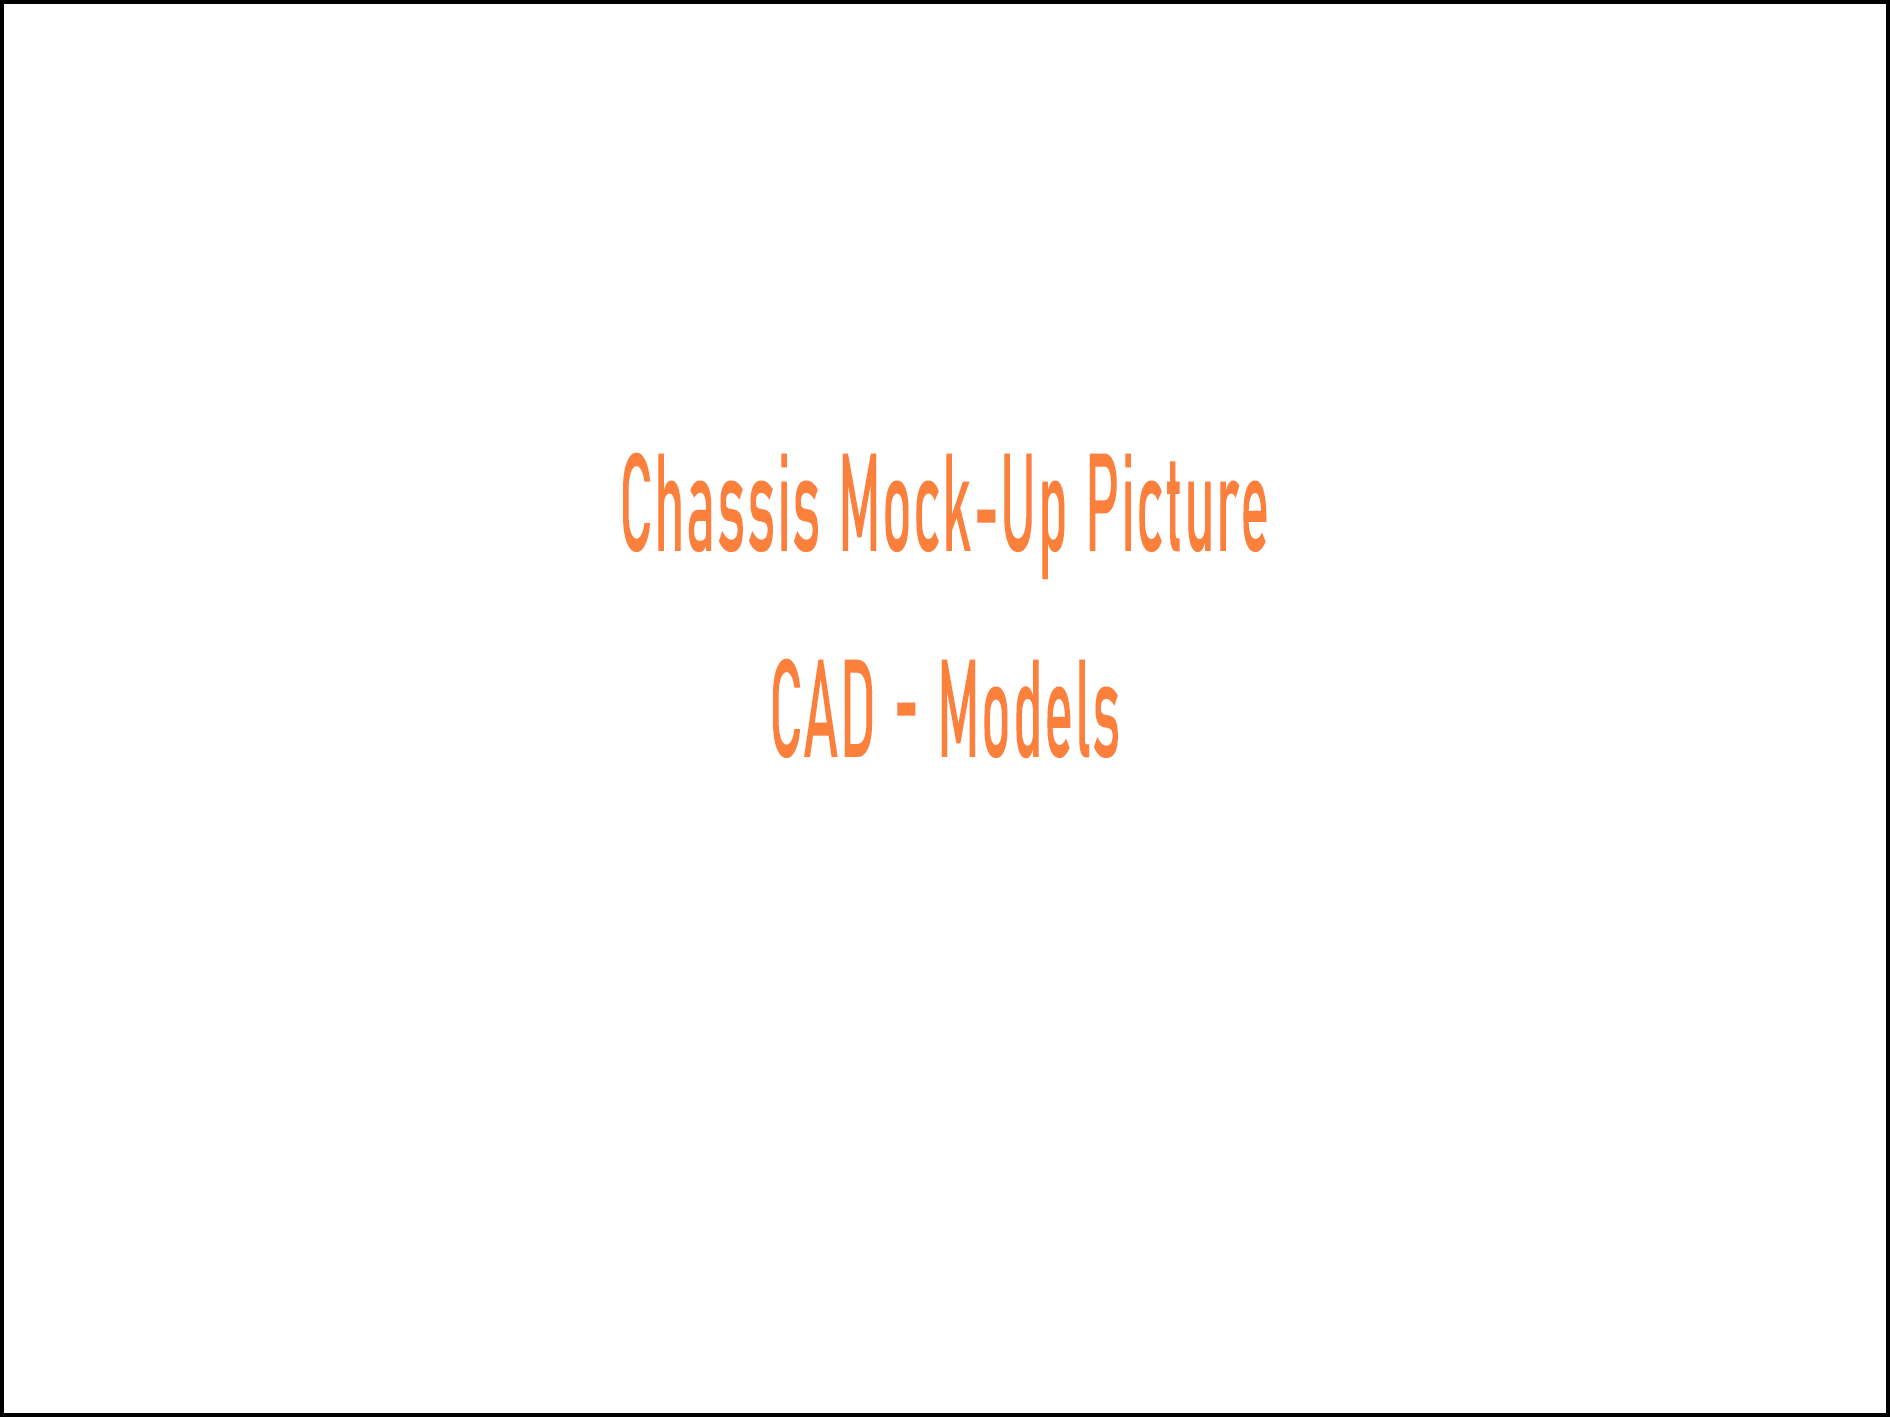
\includegraphics[width=\linewidth]{texfiles/mech/updated/chassis/cad1.png}
  \caption{Caption for the image.}
  \label{fig:image1}
\end{figure}

\begin{figure}[ht]
  \centering
  \subfloat[Caption for the first image.]{
    \centering
    \includegraphics[width=0.5\linewidth]{texfiles/mech/updated/chassis/technicaldrawing1.png}
    \label{fig:sub1}
  }
  \subfloat[Caption for the second image.]{
    \centering
    \includegraphics[width=0.5\linewidth]{texfiles/mech/updated/chassis/technicaldrawing1.png}
    \label{fig:sub2}
  }
  \caption{Caption for the whole figure.}
  \label{fig:test}
\end{figure}

\begin{figure}[ht]
  \centering
  \subfloat[Caption for the first image.]{
    \centering
    \includegraphics[width=0.5\linewidth]{texfiles/mech/updated/chassis/technicaldrawing1.png}
    \label{fig:sub1}
  }
  \subfloat[Caption for the second image.]{
    \centering
    \includegraphics[width=0.5\linewidth]{texfiles/mech/updated/chassis/technicaldrawing1.png}
    \label{fig:sub2}
  }
  \caption{Caption for the whole figure.}
  \label{fig:test}
\end{figure}

%\end{comment}


\subsubsection{Materials}

As discribed above the main factor for choosing carbon fiber sandwich panels was the the weight-strenght-cost balance. Choosing a foam-insert over a honeycomb-insert came down to the higher weather-resistants of the foam against cardboard. Again we chose carbonfiber over aluminum for the plates for lesser weight.


\subsubsection{Design Rationale}

The design rationale guiding our pod's infrastructure embodies a methodical process rooted in practical considerations and engineering principles. Our primary aim was to reduce weight from the previous design, leading us to explore the potential of carbon fiber composites.

Initially, a monocoque chassis was considered for its structural integrity, yet its high cost and manufacturing complexity deemed it impractical. Similarly, the idea of a tube chassis with carbon fiber tubes proved prohibitively expensive. Thus, we opted for a Composite Sandwich Panel Chassis, renowned for its lightweight, structural strength, and cost-effectiveness. 

Departing from the original design, which featured longitudinal panels spanning the entire length of the pod, we recognized the necessity for easy battery extraction from the side, prompting a redesign of the chassis layout. To ensure seamless panel interlocking and structural integrity, we devised a plug-in system featuring evenly distributed cutouts, meticulously aligned for connection. These connections are strengthened by precise gluing and reinforced seaming along the edges.

Additionally, crossbars were strategically integrated to fortify the chassis at suspension mounting points, mitigating potential structural weaknesses. Furthermore, close collaboration between the chassis department and other subsystems facilitated maximal compatibility and integration.

In summary, our design rationale represents a pragmatic synthesis of innovation and engineering expertise, driven by a commitment to efficiency, functionality, and cost-effectiveness.


\subsubsection{FEM Results}

\paragraph{Static Simulation Stress Test:}
In this simulation scenario, the chassis was subjected to a static stress test, replicating the forces exerted by the suspension system along with the weight of the pod. The FEM analysis yielded critical insights into the structural performance of the chassis under static loading conditions.

\paragraph{Results:}
\begin{itemize}
    \item\textbf{Maximum von Mises stress:} [Replace with your FEM result]
    \item\textbf{Maximum principal stress:} [Replace with your FEM result]
    \item\textbf{Factor of safety:} [Replace with your FEM result]
\end{itemize}

\paragraph{Interpretation: }
The FEM analysis indicates that under static loading conditions, the chassis exhibits [Replace with your interpretation of FEM results]. While localized areas may experience elevated stress levels, the overall factor of safety remains within acceptable limits, suggesting satisfactory structural integrity.

\paragraph{Braking Maneuver Simulation}
In this simulation scenario, the chassis underwent analysis with peak forces experienced during braking maneuvers, simulating the most demanding braking conditions. The FEM analysis provided crucial insights into the chassis's ability to withstand dynamic braking forces.

\paragraph{Results:}
\begin{itemize}
    \item\textbf{Maximum von Mises stress:} [Replace with your FEM result]
    \item\textbf{Maximum principal stress:} [Replace with your FEM result]
    \item\textbf{Factor of safety:} [Replace with your FEM result]
\end{itemize}

\paragraph{Interpretation: }
The FEM analysis reveals that during braking maneuvers, the chassis experiences [Replace with your interpretation of FEM results]. Despite localized stress concentrations, the overall factor of safety remains satisfactory, indicating adequate structural robustness.

\paragraph{Worst-Case Scenario:}
In the worst-case scenario simulation, the chassis was subjected to double the forces encountered in the previous scenarios, representing an extreme operating condition. This simulation aimed to assess the chassis's resilience under significantly elevated loading conditions.

\paragraph{Results:}
\begin{itemize}
    \item\textbf{Maximum von Mises stress:} [Replace with your FEM result]
    \item\textbf{Maximum principal stress:} [Replace with your FEM result]
    \item\textbf{Factor of safety:} [Replace with your FEM result]
\end{itemize}

\paragraph{Interpretation: }
The FEM analysis of the worst-case scenario indicates [Replace with your interpretation of FEM results]. Despite heightened stress levels, the factor of safety remains within acceptable limits, suggesting that the chassis can withstand double the expected forces without compromising structural integrity.

\paragraph{Conclusion:}
Overall, the FEM results provide valuable insights into the structural performance of the chassis under various loading conditions. These findings will inform further optimization efforts and ensure that the chassis meets stringent performance and reliability requirements.

%\begin{comment}
\begin{figure}[ht]
  \centering
  \includegraphics[width=\linewidth]{texfiles/mech/updated/chassis/fem1.png}
  \caption{Caption for the image.}
  \label{fig:image1}
\end{figure}

\begin{figure}[ht]
  \centering
  \subfloat[Caption for the first image.]{
    \centering
    \includegraphics[width=0.5\linewidth]{texfiles/mech/updated/chassis/fem1.png}
    \label{fig:sub1}
  }
  \subfloat[Caption for the second image.]{
    \centering
    \includegraphics[width=0.5\linewidth]{texfiles/mech/updated/chassis/fem1.png}
    \label{fig:sub2}
  }
  \caption{Caption for the whole figure.}
  \label{fig:test}
\end{figure}


\subsubsection{Calculations}

In order to ensure the accuracy and reliability of the Finite Element Method (FEM) simulations, it is crucial to provide a comprehensive justification for the simulated loads. The following reasoning and calculations support the chosen loads for each simulation scenario:

\begin{itemize}
  \item \textbf{Static Simulation Stress Test}
    \begin{itemize}
      \item \textbf{Reasoning:} The static simulation stress test replicates the forces exerted by the 		suspension system and the weight of the pod when the vehicle is at rest or moving at a 					constant velocity. This scenario is essential to evaluate the chassis's ability to withstand 				static loading conditions, providing insights into its structural integrity and load-bearing 				capacity.

	  \item \textbf{1.	Suspension Forces:} 
		The suspension system applies forces to the chassis, primarily in the vertical direction, to 				support the weight of the vehicle and absorb road irregularities.

	  \item \textbf{Average Suspension Force (Fsus):}
		(Insert calculation based on suspension design and vehicle weight distribution)

	  \item \textbf{2.	Weight of the Pod:} 
		The weight of the pod contributes to the overall static loading on the chassis.

	  \item \textbf{Pod Weight (Wpod):} 
		(Insert actual weight of the pod)

	  \item \textbf{Total Load:}
		Total Load = Suspension Forces + Weight of the Pod Total Load = Fsus + Wpod
	\end{itemize}
\end{itemize}

\begin{itemize}
  \item \textbf{Braking Maneuver Simulation}
    \begin{itemize}
      \item \textbf{Reasoning:} The braking maneuver simulation replicates the peak forces experienced 		by the chassis during braking events. This scenario is crucial to assess the chassis's ability 		to withstand dynamic loading conditions, particularly during sudden deceleration, and ensure 				structural stability and safety.

	  \item \textbf{1.	Peak Braking Force:} 
		The braking system applies forces to the chassis during braking maneuvers, primarily in the 				longitudinal direction, to decelerate the vehicle.

	  \item \textbf{Peak Braking Force (Fbrake):}
		(Insert calculation based on braking system specifications and vehicle weight)
	\end{itemize}
\end{itemize}
	
\begin{itemize}  
  \item \textbf{Worst-Case Scenario:}
	\begin{itemize}
	  \item \textbf{Reasoning:} The worst-case scenario involves doubling the forces encountered in 				the previous scenarios, representing an extreme operating condition. This scenario tests the 				limits of the chassis's structural resilience and provides insights into its performance under 		significantly elevated loading 
		conditions.

	  \item \textbf{1.	Double Suspension Forces:} The suspension forces are doubled to simulate 					extreme vertical loading conditions on the chassis.
-	Double Suspension Forces (2 * Fsus)

	  \item \textbf{1.	Double Braking Forces:}The braking forces are doubled to simulate extreme 				braking maneuvers.
-	Double Braking Forces (2 * Fbrake)

	  \item \textbf{Conclusion:} By providing rigorous justification and performing the necessary load 		calculations, we ensure that the simulated loads accurately represent real-world operating 				conditions. These simulations enable us to evaluate the structural performance of the chassis 				under various loading scenarios, guiding optimization efforts and ensuring the chassis meets 				stringent performance requirements.

	\end{itemize}
\end{itemize}


-	Acceleration due to gravity: \(9.81\frac{m}{s^2}\)
-	Weight of the pod (W\_pod) = Mass of the pod × Acceleration due to gravity

2.	Forces from Suspension:
-	Suspension force: [Replace with actual suspension force]
-	Total force from suspension (F\_suspension) = Suspension force × Number of suspension points

3.	Total Static Load:
-	Total static load = Weight of the pod + Total force from suspension

Simulation Scenario 2: Braking Maneuver Simulation

1.	Peak Braking Force:
-	Maximum deceleration: [Replace with actual maximum deceleration]
-	Mass of the vehicle: [Replace with actual mass]
-	Peak braking force = Mass of the vehicle × Maximum deceleration

Worst-Case Scenario:

1.	Double Forces:
-	Double weight of the pod: 2 × Weight of the pod
-	Double total


\subsubsection{Mesh and Boundary Conditions}

Mesh Type: For our Finite Element Method (FEM) simulations, we utilized a structured mesh approach, specifically employing a combination of hexahedral and tetrahedral elements. This mesh type offers several advantages, including improved computational efficiency, better accuracy in capturing complex geometries, and reduced numerical error.

Boundary Conditions:

1.	Fixed Constraints:
-	Suspension Mounting Points: The chassis is fixed at the suspension mounting points to simulate the rigid attachment of the suspension system to the chassis.
-	Ground Contact: The bottom surface of the chassis is fixed to simulate contact with the ground, ensuring realistic loading conditions.

2.	Applied Loads:
-	Suspension Forces: Vertical forces are applied at the suspension mounting points to simulate the forces exerted by the suspension system on the chassis. These forces represent the weight of the vehicle and any additional loads imposed by the suspension system.
-	Braking Forces: Longitudinal forces are applied to simulate the braking forces exerted on the chassis during braking maneuvers. These forces are applied at the contact points between the braking system and the chassis.

3.	Symmetry and Constraints:
-	Symmetry: Symmetry boundary conditions are applied to exploit the symmetry of the chassis geometry, reducing computational complexity and improving efficiency.
-	Constraints: Constraints are imposed on certain degrees of freedom to enforce realistic behavior and prevent unrealistic deformations or displacements.

4.	Mesh Refinement:
-	Local Mesh Refinement: Mesh refinement techniques are applied in areas of geometric complexity or high stress concentration to ensure accurate representation of stress distribution and structural response.

Conclusion: By employing a structured mesh approach and carefully defining boundary conditions, we ensure that our FEM simulations accurately capture the behavior of the chassis under various loading scenarios. These simulations provide valuable insights into the structural performance of the chassis, guiding optimization efforts and ensuring that the design meets stringent performance requirements.

\textbf{WILL BE ADDED SOON}

\begin{comment}
\begin{figure}[ht]
  \centering
  \subfloat[Caption for the first image.]{
    \centering
    \includegraphics[width=0.5\linewidth]{texfiles/mech/updated/chassis/mesh1.png}
    \label{fig:sub1}
  }
  \subfloat[Caption for the second image.]{
    \centering
    \includegraphics[width=0.5\linewidth]{texfiles/mech/updated/chassis/mesh1.png}
    \label{fig:sub2}
  }
  \caption{Caption for the whole figure.}
  \label{fig:test}
\end{figure}
\end{comment}




\subsection{Manufacturing Process}

Firstly, the panels are sourced and procured in accordance with precise specifications, ensuring they meet the required size and shape criteria. Any necessary cutouts or holes are meticulously made in alignment with design specifications, utilizing advanced cutting techniques to ensure accuracy and consistency. Subsequently, support plates are precisely cut to the required size and shape, with corresponding holes carefully drilled to facilitate seamless integration with the panels. 

These support plates serve a critical role in reinforcing the structural integrity of the chassis, providing additional strength and stability. Following preparation of the panels and support plates, a meticulous assembly process ensues. The support plates are methodically glued to the designated spots on the panels, adhering to precise positioning guidelines to ensure optimal alignment and functionality.

Once the support plates are securely affixed, the panels are carefully assembled and glued together, forming a cohesive structure that embodies the desired design configuration. This assembly process is executed with meticulous attention to detail, ensuring that each component is seamlessly integrated to achieve the desired structural integrity and functionality.

Finally, the seams between the assembled panels are meticulously cut to the required size and adhered to the edges of the plugged panels. This final step serves to further reinforce the structural integrity of the chassis while providing a polished finish that enhances both aesthetics and durability. Through adherence to this comprehensive manufacturing process, we ensure that the designed part is not only realized in a practical and efficient manner but also upholds the highest standards of quality and performance.

\textbf{or:}

Efforts have been undertaken to ensure that the designed part is realistically manufacturable, with a focus on simplicity, efficiency, and accessibility in manufacturing processes.

1.	2D Waterjet Cutting for Panels: Utilizing 2D waterjet cutting for the panels ensures precise and efficient fabrication. This method allows for accurate cutting of complex shapes and contours, facilitating the production of panels with minimal material wastage.

2.	Scissor-Cut Seams: Seam cutting by scissors offers a straightforward and cost-effective approach to joining panels. This manual method provides flexibility and ease of assembly, allowing for adjustments as needed during the manufacturing process. Additionally, it eliminates the need for specialized equipment, reducing production costs and complexity.

3.	Waterjet Cutting for Plates: Employing waterjet cutting for the plates ensures accurate and clean cuts, maintaining dimensional accuracy and quality. This method allows for the fabrication of support plates with intricate designs and precise hole placements, enabling optimal integration with the chassis components.

By leveraging these manufacturing techniques, we streamline the production process while maintaining the integrity and functionality of the designed part. The simplicity and accessibility of these methods ensure that the manufacturing process remains efficient, cost-effective, and scalable, ultimately contributing to the overall success of the project.




\subsection{Integration process}


\subsubsection{Assembling}

Firstly, the panels are sourced and procured in accordance with precise specifications, ensuring they meet the required size and shape criteria. Any necessary cutouts or holes are meticulously made in alignment with design specifications, utilizing advanced cutting techniques to ensure accuracy and consistency.

Subsequently, support plates are precisely cut to the required size and shape, with corresponding holes carefully drilled to facilitate seamless integration with the panels. These support plates serve a critical role in reinforcing the structural integrity of the chassis, providing additional strength and stability.

Following preparation of the panels and support plates, a meticulous assembly process ensues. The support plates are methodically glued to the designated spots on the panels, adhering to precise positioning guidelines to ensure optimal alignment and functionality.

Once the support plates are securely affixed, the panels are carefully assembled and glued together, forming a cohesive structure that embodies the desired design configuration. This assembly process is executed with meticulous attention to detail, ensuring that each component is seamlessly integrated to achieve the desired structural integrity and functionality.

Finally, the seams between the assembled panels are meticulously cut to the required size and adhered to the edges of the plugged panels. This final step serves to further reinforce the structural integrity of the chassis while providing a polished finish that enhances both aesthetics and durability.

Through adherence to this comprehensive manufacturing process, we ensure that the designed part is not only realized in a practical and efficient manner but also upholds the highest standards of quality and performance.

\subsubsection{Assembly interaction}


The interaction between subsystems within the pod is orchestrated with precision, each component playing a crucial role in ensuring seamless functionality and performance. At the heart of this interaction lies the chassis, serving as the sturdy backbone upon which all subsystems are mounted. The chassis not only provides structural support but also serves as a conduit for distributing forces generated by key subsystems such as the brakes, motor, and suspension.

The motor, positioned centrally within the pod, exerts significant forces that are channeled directly through the chassis. As the primary source of propulsion, the motor's torque and power output directly influence the chassis's stability and performance. Similarly, the braking system, situated on the sides directly above the track, exerts substantial forces during deceleration. These forces are transmitted through the chassis, requiring robust structural reinforcement to withstand the resulting stresses.

The suspension system, located at the front and back ends of the pod, plays a critical role in ensuring ride comfort and handling. The forces generated by the suspension, particularly during cornering and uneven terrain traversal, are transmitted through the chassis, necessitating careful design considerations to maintain stability and responsiveness.

In addition to these dynamic subsystems, the electrical systems are integrated into the chassis using sheet metal and 3D-printed brackets. This strategic mounting ensures secure placement while minimizing interference with other components.

Furthermore, the battery, housed within a dedicated battery box, is mounted on telescopic rails affixed to the chassis. This arrangement not only facilitates easy access for maintenance but also ensures optimal weight distribution and stability.

Through integration and strategic mounting, each subsystem interacts harmoniously with the chassis and other components, collectively contributing to the overall functionality and performance of our pod. This cohesive interaction is essential for achieving our objectives of efficiency, reliability, and safety.




\subsection{Safety Considerations}


\subsubsection{Safety Factor}

For our project, we have established a minimum safety factor of n=2 for all structural elements. This means that the ultimate strength of each component must be at least twice the maximum expected load it will experience.

Reaching a safety factor of n=… provides a significant margin of safety, offering protection against unforeseen variations in loading conditions, material properties, and environmental factors. It ensures that the structural elements can withstand unexpected peak loads or transient events without compromising safety or integrity.


\subsubsection{Worst-Case Scenarios}

\textbf{WILL BE ADDED SOON}




\subsection{FMEA Results Discussion}


\subsubsection{Risk Assessment}

\textbf{WILL BE ADDED SOON}


\subsubsection{FMEA and Risk Mitigation}
\begin{comment}
\textbf{WILL BE ADDED SOON}
\begin{figure}[ht]
  \centering
  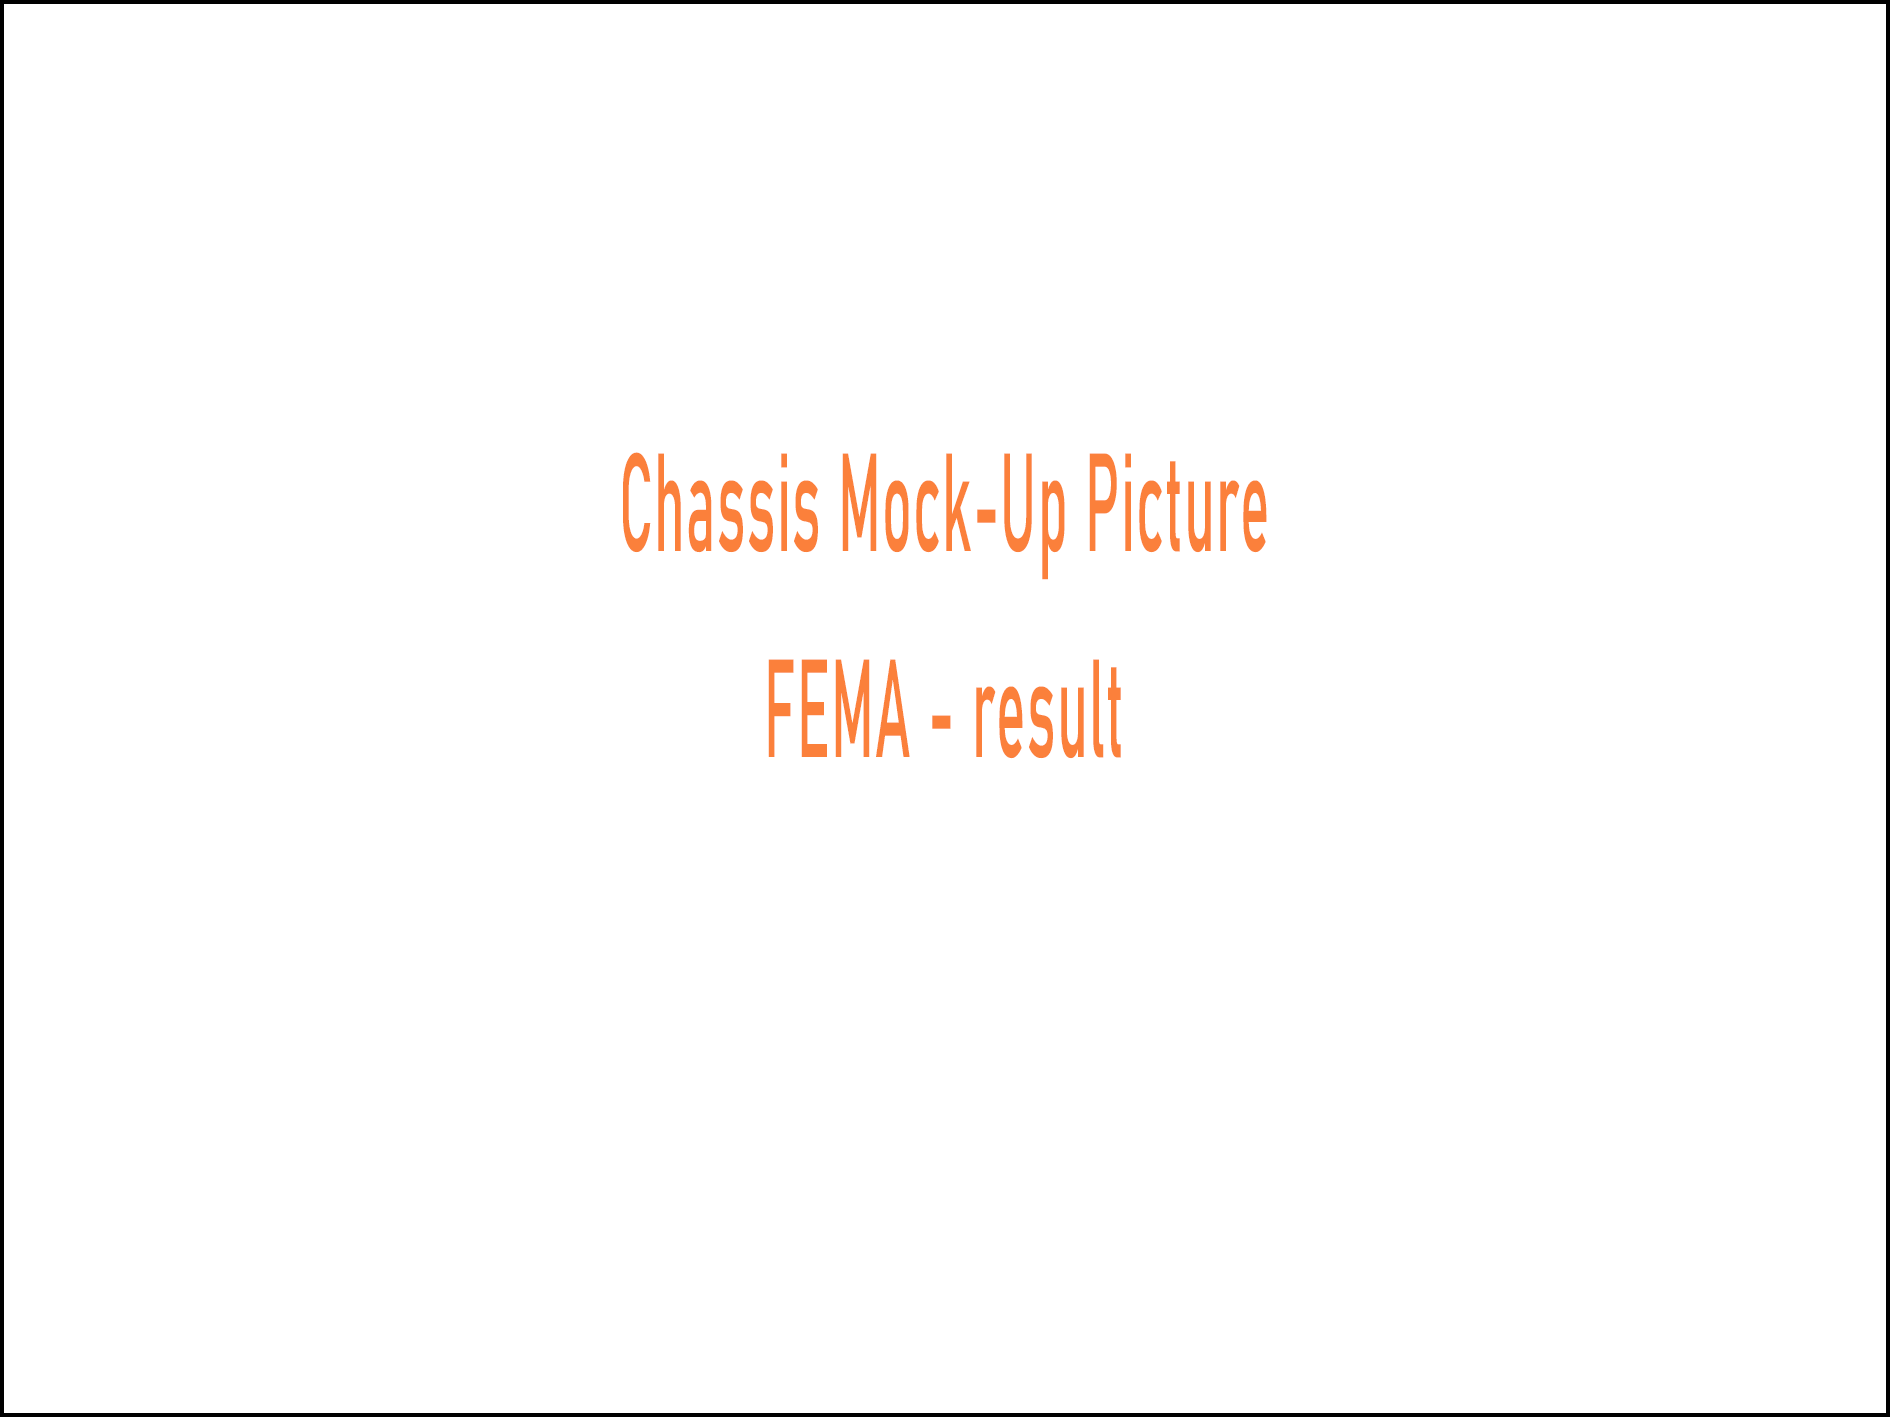
\includegraphics[width=\linewidth]{texfiles/mech/updated/chassis/FMEA1.png}
  \caption{Caption for the image.}
  \label{fig:image1}
\end{figure}
\end{comment}

\subsubsection{Simulation Evidence}

\textbf{WILL BE ADDED SOON}




\subsection{Testing}


\subsubsection{Safety Procedures Documentation}

The testing procedures for the hyperloop pod chassis are meticulously crafted to assess structural integrity, durability, and performance under conditions that closely simulate actual operation. The procedures outlined below provide a comprehensive approach to validating the chassis design.

\paragraph{Static Load Testing}
\begin{itemize}
    \item \textbf{Objective:} To evaluate the chassis's ability to withstand forces it would encounter while stationary.
    \item \textbf{Procedure:} Securely mount the chassis at suspension mounting holes. Apply a static load equivalent to twice the anticipated weight of the finished pod.
    \item \textbf{Outcome:} Determine load-bearing capacity and ensure no structural deformation or failure.
\end{itemize}

\paragraph{Dynamic Load Testing}
\begin{itemize}
    \item \textbf{Objective:} To assess the chassis's responsiveness and robustness under dynamic loading conditions.
    \item \textbf{Procedure:} Subject the chassis to simulated forces of acceleration, braking, and cornering. Collect data on how the chassis flexes and reacts under these conditions.
    \item \textbf{Outcome:} Confirm the chassis's integrity under dynamic stresses and identify potential areas for reinforcement.
\end{itemize}

\paragraph{Bending Stress Test}
\begin{itemize}
    \item \textbf{Objective:} To understand the material properties of the chassis, particularly its bending strength and ductility.
    \item \textbf{Procedure:} Fabricate a reference part from the same material as the chassis. Apply incremental force until the part fails, if applicable.
    \item \textbf{Outcome:} Ascertain the material's resistance to bending forces and its behavior under stress.
\end{itemize}

\paragraph{Vibration Testing}
\begin{itemize}
    \item \textbf{Objective:} To evaluate the chassis's ability to endure and dampen vibrations during operation.
    \item \textbf{Procedure:} Expose the chassis to controlled vibrations at various frequencies and amplitudes to simulate motor-generated vibrations and other operational scenarios.
    \item \textbf{Outcome:} Ensure the chassis can effectively dampen vibrations and avoid resonance or structural fatigue.
\end{itemize}


\subsubsection{preliminary testing plan}

This section outlines the testing plan for the chassis of the hyperloop pod, ensuring its structural integrity and stability under various loads and conditions.

\paragraph{Static Load Testing}
\begin{itemize}
    \item \textbf{Method:} Securely mount the chassis at the suspension mounting holes.
    \item \textbf{Loading:} Apply a static load equivalent to twice the weight of the finished pod.
    \item \textbf{Duration:} Maintain the load for a predetermined period to assess the structural integrity.
    \item \textbf{Measurement:} Monitor for deformation or failure.
\end{itemize}

\paragraph{Dynamic Load Testing}
\begin{itemize}
    \item \textbf{Method:} Simulate dynamic forces experienced during operation.
    \item \textbf{Loading:} Apply forces to replicate acceleration, braking, and cornering.
    \item \textbf{Duration:} Perform over various speeds and conditions.
    \item \textbf{Measurement:} Record deflection and structural response.
\end{itemize}

\paragraph{Bending Stress Test}
\begin{itemize}
    \item \textbf{Method:} Use a reference part made from the same material as the chassis panels.
    \item \textbf{Loading:} Incrementally apply force until failure.
    \item \textbf{Measurement:} Note the force applied and deformation at failure.
    \item \textbf{Expected Result:} Determine material's bending strength and ductility.
\end{itemize}

\paragraph{Vibration Testing}
\begin{itemize}
    \item \textbf{Method:} Subject chassis to controlled vibrations across frequencies.
    \item \textbf{Loading:} Simulate operational vibrations.
    \item \textbf{Duration:} Extend testing for durability assessment.
    \item \textbf{Measurement:} Assess chassis damping and response to vibrations.
    \item \textbf{Expected Result:} Ensure chassis can maintain integrity under vibration.
\end{itemize}

\paragraph{Expected Results}
The chassis is expected to demonstrate stability and maintain structural integrity under static and dynamic loads. The bending stress test will confirm the material's properties, while vibration testing will validate damping capabilities. Through this comprehensive testing, the chassis will be proven to meet rigorous quality and safety standards, crucial for the hyperloop pod's performance.



\section{Suspension}

\subsection{Introduction}
\subsubsection{Overview of the System}
The front and rear double wishbone suspension system serves as a critical component within our Hyperloop pod, aimed at delivering a comfortable and stable ride experience. At its core lies the circular knuckle, meticulously designed to accommodate essential parts like bearings, retaining rings, and shafts. This central hub enables smooth vertical movement of the suspension, absorbing track imperfections for a seamless ride. Wishbones attached to the knuckle control suspension motion, featuring specialized bearings to maintain precise alignment. Dampeners directly connected to the knuckle assembly absorb shocks and vibrations, enhancing responsiveness to terrain changes. Additionally, a linkage mechanism minimizes lateral movement, ensuring stability, especially during high-speed travel. Integration with the chassis is facilitated by high-performance bearings, allowing for articulation and load transfer.

\subsubsection{Requirements and Constraints}
The suspension system must meet stringent requirements to ensure optimal performance and safety. It must provide exceptional ride quality, stability, and control throughout the journey, from acceleration to high-speed cruising. Constraints include optimizing weight distribution and reducing unsprung mass to enhance handling dynamics. The system must also minimize lateral sway and maintain course stability under demanding conditions. Incorporation of specialized bearings like the Female Wiebel Bearing further enhances stability and control. Meticulous engineering is essential to meet these requirements while adhering to space, weight, and durability constraints inherent to Hyperloop pod design.

\newpage
\subsection{Subsystem Overview}
\subsubsection{Explanation of Subsystem Concepts}
\textbf{Control Arms:} The control arms are the primary components of the double wishbone suspension system, forming the distinctive "double wishbone" shape. These arms connect the Knuckle to the vehicle's chassis, with one arm positioned above and another below the wheel. They work together to control the wheel's vertical movement and maintain stability. This configuration allows the control arms to absorb bumps and shocks from the road while providing precise control over the wheel's motion.

\textbf{Shock Absorbers (Dampers):} Shock absorbers control the rate of compression and expansion of the springs, damping the oscillations of the suspension system caused by road imperfections. Shock absorbers play a crucial role in enhancing stability, comfort, and control by minimizing bounce and sway.

\newpage
\subsection{Theoretical Concepts}
\subsubsection{Detailed Explanation of Theoretical and Physical Principles}
\textbf{Theoretical Principles:}

\begin{enumerate}
    \item \textbf{Independent Suspension:}
    
    A fundamental theoretical principle underlying the double wishbone suspension is the provision of independent movement for each wheel. By decoupling the motion of one wheel from the other, this system ensures that disturbances affecting one wheel do not directly impact the other. This independence is crucial for maintaining optimal traction, stability, and comfort, particularly when navigating uneven terrain or cornering at high speeds. With independent suspension, variations in road surface or cornering forces can be effectively managed, enhancing overall vehicle dynamics.
    
\item \textbf{Controlled Wheel Movement:}
    
    The design of the wishbone-shaped control arms serves to control the movement of the wheel in multiple directions. These arms dictate the wheel's motion both vertically, for absorbing bumps and shocks, and horizontally, for steering input and stability. By strategically positioning and shaping the control arms, engineers can tailor the suspension's response to different driving conditions, ensuring precise handling and ride quality. This controlled movement allows for optimized wheel alignment, minimizing tire wear and maximizing grip, leading to improved overall performance and safety.
\end{enumerate}

\textbf{Physical Principles:}

\begin{enumerate}
    \item \textbf{Shock Absorption:}
    
    Shock absorption is a primary physical principle at work in a double wishbone suspension system. When the wheel encounters bumps or irregularities on the road surface, the suspension compresses and decompresses to absorb the impact. This process involves the coordinated action of the control arms and the shock absorbers (typically coilover or strut-type). The control arms guide the wheel's vertical movement, while the shock absorbers dampen the oscillations generated by road disturbances. Together, they mitigate the transmission of vibrations and shocks to the vehicle's chassis, providing occupants with a smoother and more comfortable ride experience.
    
    \item \textbf{Load Distribution and Handling:}
    
    Load distribution and handling are essential physical principles influenced by the double wishbone suspension design. By distributing the vehicle's weight more evenly across all four wheels, this suspension system enhances traction and stability, especially during acceleration, braking, and cornering maneuvers. The geometry of the control arms plays a critical role in determining the vehicle's handling characteristics. Optimal geometry helps manage weight transfer during dynamic driving situations, ensuring responsive steering, minimal body roll, and enhanced cornering ability. Additionally, the precise control over wheel movement provided by the double wishbone setup contributes to predictable and balanced handling, promoting driver confidence and safety on the road.
\end{enumerate}

\newpage
\subsubsection{Use of Free Body Diagrams for Load Cases}
\begin{figure}[ht!]
  \centering
  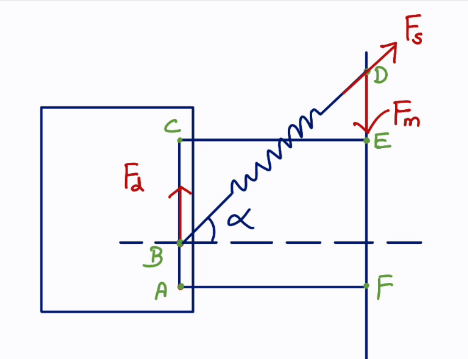
\includegraphics[width=\linewidth]{texfiles/mech/eimg/suspension/fbd.png}
  \caption{Caption for the image.}
  \label{fig:image1}
\end{figure}

\newpage
\begin{align*}
1. & \text{ Fs:} & \text{Force of Shock Absorber} \\
2. & \text{ Fd:} & \text{Force due to disturbances} \\
3. & \text{ Fm:} & \text{Force to weight of the Chassis} \\
4. & \alpha: & \text{Horizontal angle of the Shock Absorber} \\
5. & \text{ CE:} & \text{Upper Wishbone} \\
6. & \text{ AF:} & \text{Lower wishbone} \\
7. & \text{ AC:} & \text{Knuckle} \\
\end{align*}

\subsection{Design Process and Appearance}
\subsubsection{Presentation of CAD Models and Technical Drawings}
\begin{figure}[ht!]
  \centering
  \begin{subfigure}{.5\textwidth}
    \centering
    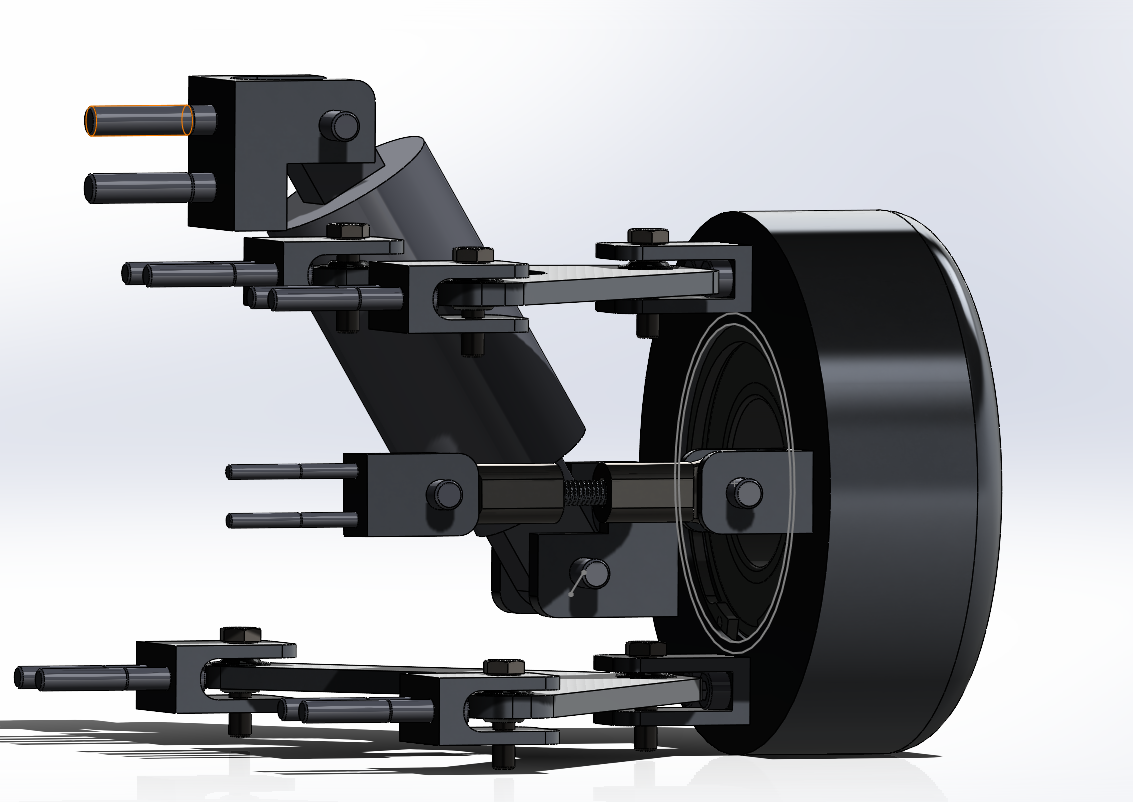
\includegraphics[width=\linewidth]{texfiles/mech/eimg/suspension/CAD_Deign of Rear Suspension.png}
    \caption{Caption for the first image.}
    \label{fig:sub1}
  \end{subfigure}%
  \begin{subfigure}{.5\textwidth}
    \centering
    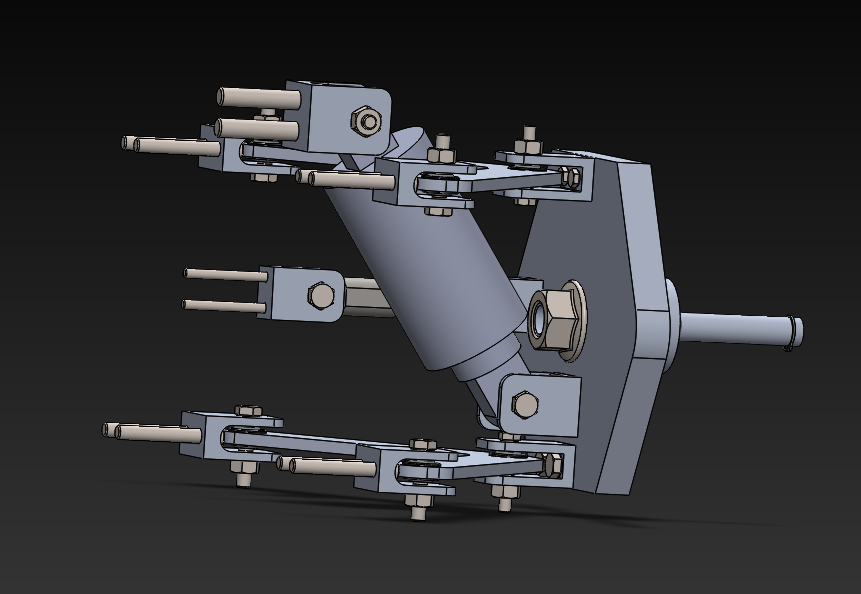
\includegraphics[width=\linewidth]{texfiles/mech/eimg/suspension/CAD Design Front wishbone Assembly.png}
    \caption{Caption for the second image.}
    \label{fig:sub2}
  \end{subfigure}%
\end{figure}
\newpage
\subsubsection{Justification of Material Selection}

\begin{itemize}
    \item \textbf{High Strength-to-Weight Ratio:} Utilizing Alloy 6061 would help reduce the overall weight of your suspension components while maintaining the necessary strength. This can improve the performance of your vehicle by reducing unsprung mass, which enhances handling, responsiveness, and fuel efficiency.
    
    \item \textbf{Corrosion Resistance:} The corrosion resistance of Alloy 6061 ensures the longevity and durability of your suspension components, especially considering the exposure to various environmental conditions and road debris that they may experience.
    
    \item \textbf{Weldability and Formability:} Alloy 6061's weldability and formability allow for the fabrication of complex and precisely shaped suspension components. This flexibility in manufacturing processes can help optimize the design of your suspension system for improved performance and reliability.
    
    \item \textbf{Heat Treatability:} Heat treatability provides the opportunity to enhance specific mechanical properties of your suspension components, such as strength and hardness. This can be particularly useful for critical components that undergo significant loads or stress during operation.
    
    \item \textbf{Cost-Effectiveness:} Alloy 6061 offers a cost-effective solution for your suspension system without compromising on quality or performance. This ensures that you can achieve your desired suspension characteristics while keeping manufacturing costs within budget.
    
    \item \textbf{Recyclability:} The recyclability of Alloy 6061 aligns with sustainability efforts and reduces environmental impact. Using a recyclable material for your suspension components contributes to the overall eco-friendliness of your vehicle's design.
\end{itemize}

\subsubsection{Presentation of Material Properties}
\begin{table}[H]
\centering
\caption{Properties of Alloy 6061}
\begin{tabular}{@{}ll@{}}
\toprule
\textbf{Property} & \textbf{Value} \\
\midrule
Yield Strength & 35 ksi (240 MPa) \\
Elongation at Break & 10\% \\
Fatigue Strength & 96 MPa (14 $\times$ 10\textsuperscript{3} psi) \\
Brinell Hardness & 93 \\
Young’s Modulus & 69 GPa (10 $\times$ 10\textsuperscript{6} psi) \\
Thermal Conductivity & 167 W/m$\cdot$K \\
Melting Point & 582°C (1080°F) \\
Heat Treating & Solution heat-treated (6061-W) \\
\bottomrule
\end{tabular}
\end{table}

\subsubsection{Presentation of Finite Element Method (FEM) Results}
\begin{figure}[H]
  \centering
  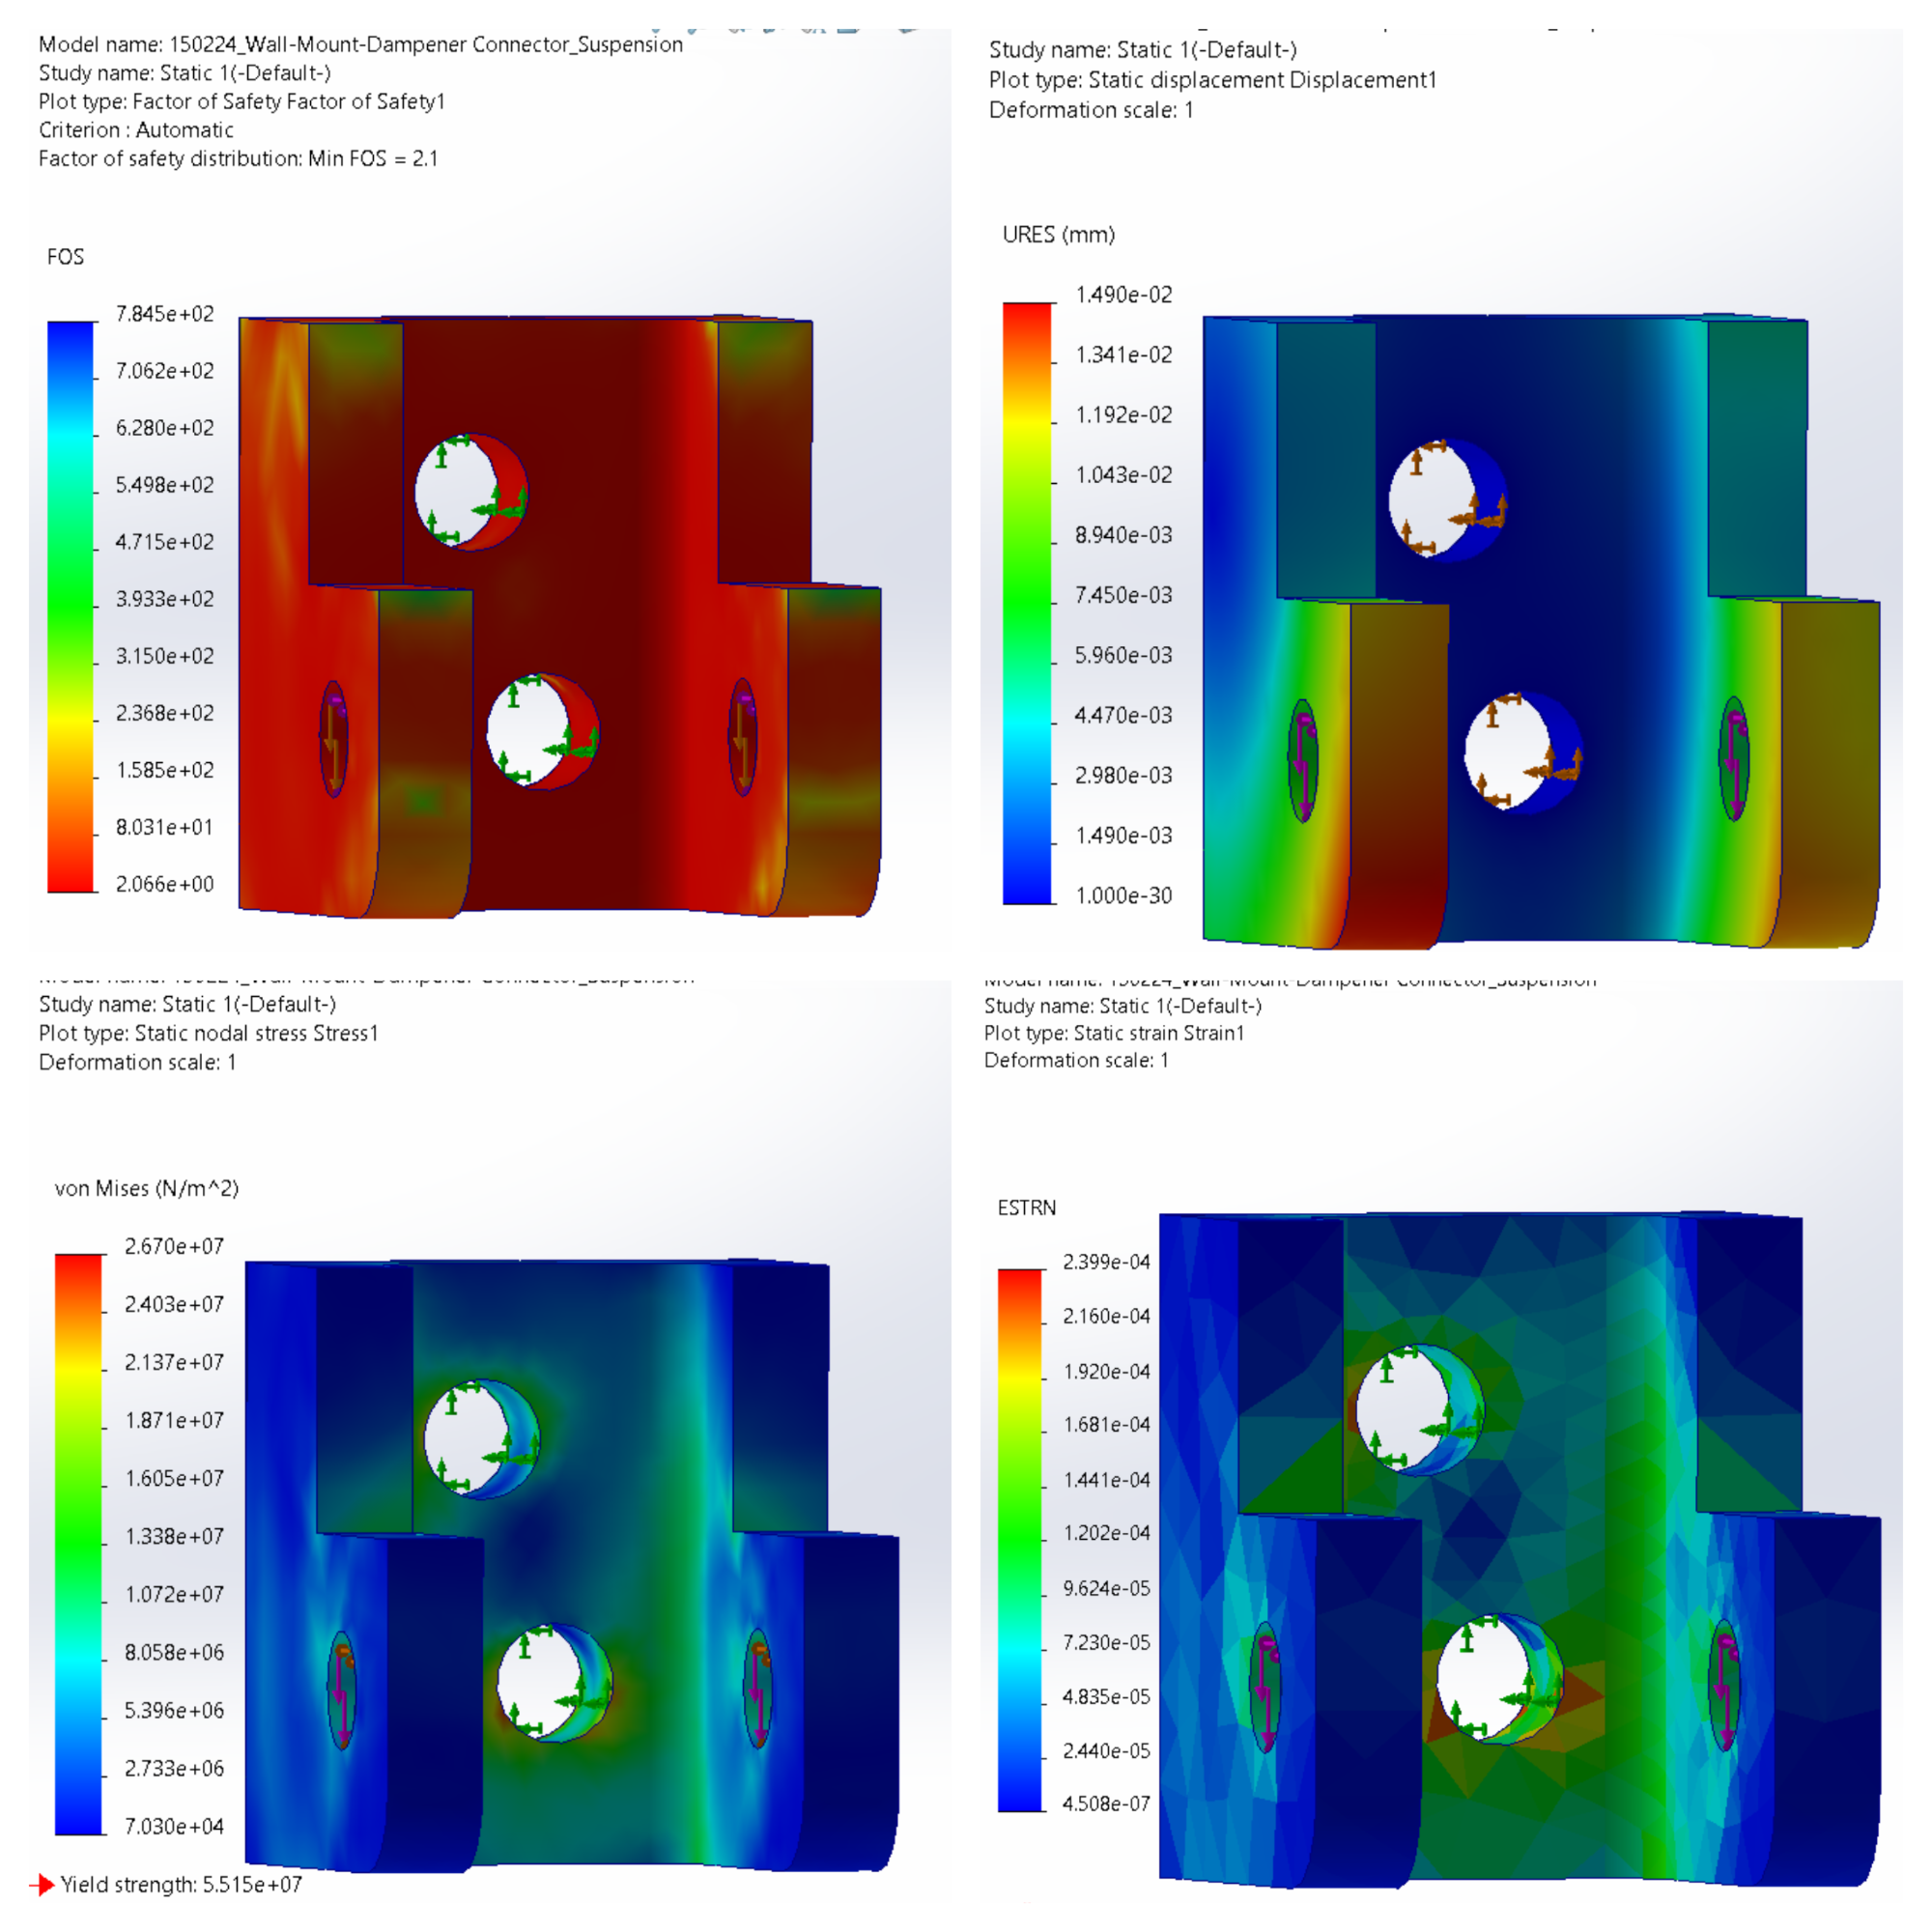
\includegraphics[width=\linewidth]{texfiles/mech/eimg/suspension/Mounting FEM results.png}
  \caption{Caption for the image.}
  \label{fig:image1}
\end{figure}


\begin{table}[H] % <-- Use [H] option to place the table exactly here
\centering
\caption{Mesh Information - Details}
\begin{tabular}{@{}ll@{}}
\toprule
\textbf{Parameter} & \textbf{Value} \\
\midrule
Total Nodes & 7097 \\
Total Elements & 4125 \\
Maximum Aspect Ratio & 6.3707 \\
\% of Elements with Aspect Ratio $<$ 3 & 99.2 \\
\bottomrule
\end{tabular}
\end{table}

This study presents a Finite Element Analysis (FEA) conducted to evaluate the structural integrity and performance of the shock absorber mounting configuration on the knuckle of a rear double wishbone suspension system. The primary objective was to assess the adequacy of the mounting design in withstanding applied forces and ensuring safety during operation. Initial simulations revealed areas of concern regarding the thickness of the mounting, prompting adjustments to the design parameters. Subsequent iterations were carried out to optimize the configuration, resulting in a revised model with enhanced strength characteristics. Through comprehensive analysis, a safety factor of 2 was achieved, indicating satisfactory resistance to anticipated loads. The findings of this study contribute to the understanding of structural behavior in automotive suspension systems and inform design improvements for enhanced performance and reliability (see Figure~\ref{fig:figure1}).




\newpage
\subsection{Manufacturing Process}
\subsubsection{Compilation of Parts List}
\begin{table}[H]
\centering
\caption{Component Specifications}
\begin{tabular}{|l|l|l|l|l|l|}
\hline
\textbf{Component} & \textbf{Number [-]} & \textbf{Mass [kg]} & \textbf{Size [mm x mm x mm]} & \textbf{Material} & \textbf{Manufacturing process} \\ \hline
Rear Wheels & x2 & - & $\phi$ 200 x 155 & Aluminum Alloy 6061 & In-house \\ \hline
Front Wheels & x2 & - & $\phi$ 200 x 50 & Galvanized Steel & Rollenplus.de (Outsourced) \\ \hline
Rear Knuckle & x2 & 1.473 & $\phi$ 145 x 52 & Aluminum Alloy 6061 & In-house \\ \hline
Cylindrical Roller Bearing Rear Knuckle & x4 & - & $\phi$ 85 x 18.6 & 100Cr6 & Outsourced \\ \hline
Retaining Ring DIN 472 & x4 & - & $\phi$ 85 & Spring Steel & Mädler (Outsourced) \\ \hline
Rear Upper Wishbone & x2 & 0.08896 & 119 x 102 x 6 & Aluminum Alloy 6061 & In-house \\ \hline
Rear Lower Wishbone & x2 & 0.1255 & 224 x 102 x 6 & Aluminum Alloy 6061 & In-house \\ \hline
Shock Absorber & x4 & - & $\phi$ 45 x 150 & - & XLC (Outsourced) \\ \hline
Wishbone Wall Mount & x16 & 0.02441 & 36 x 30 x 18 & Aluminum Alloy 6061 & In-house \\ \hline
Knuckle Wishbone Mount & x8 & 0.02055 & 37 x 25 x 18 & Aluminum Alloy 6061 & In-house \\ \hline
Rear Shock Absorber Mounts & x4 & 0.05583 & 40 x 40 x 35 & Aluminum Alloy 6061 & In-house \\ \hline
Linkage Mounts & x8 & 0.0135 & 31.75 x 22 x 18 & Aluminum Alloy 6061 & In-house \\ \hline
Female Rod End Bearing & x8 & - & 47 x 16 x 14 & Stainless Steel 1.4301 & Mädler (Outsourced) \\ \hline
Linkage Connecting Rod & x4 & 0.0032 & $\phi$ 7 x 43 & Aluminum Alloy 6061 & In-house \\ \hline
Uni Ball Bearings & x24 & - & $\phi$ 16 x 9 & 100Cr6 & Mädler (Outsourced) \\ \hline
Front Wheel Hub & x2 & 0.10959 & $\phi$ 40 x 115 & Aluminum Alloy 6061 & In-house \\ \hline
Front Wishbones & x2 & 0.09553 & 224 x 102 x 6 & Aluminum Alloy 6061 & In-house \\ \hline
Front Knuckle & x2 & 0.65721 & $\phi$ 160 x 15 & Aluminum Alloy 6061 & In-house \\ \hline
Front Shock Absorber Mounts & x4 & 0.01952 & 36 x 32 x 28 & Aluminum Alloy 6061 & In-house \\ \hline
Retaining Ring DIN 471 & x2 & - & $\phi$ 11 & Spring Steel & Mädler (Outsourced) \\ \hline
\end{tabular}
\end{table}

\subsubsection{Description of Efforts for Realistic Manufacturability}

Efforts for realistic manufacturability focus on optimizing production processes for critical suspension components, ensuring precision, reliability, and cost-effectiveness. This includes employing advanced manufacturing techniques and methodologies tailored to specific components, enhancing both efficiency and quality throughout the production process.

\subsubsection{Explanation of Manufacturing Techniques}


\textbf{Knuckle Manufacturing:} For the knuckle manufacturing process, a combination of water jet spray technology and CNC machining will be employed to ensure precise fabrication of critical features. The main hole for the shaft will be created using water jet spray technology, guaranteeing accuracy and efficiency in alignment and fitment. Additionally, advanced CNC machining will be utilized for creating internal grooves within the knuckle to accommodate the cylindrical roller bearings, ensuring precise dimensions and tolerances for proper seating and functionality of components.

\textbf{Wishbone Manufacturing:} Wishbones will be manufactured utilizing water jet spray technology, allowing for precise cutting of materials and efficient production. This ensures uniformity and consistency in the manufacturing process, resulting in high-quality wishbones that meet strict performance standards.

\textbf{Linkage Rod Manufacturing:} The linkage rod will undergo precision threading using a lathe machine, ensuring accurate fitment and functionality within the suspension system. This process guarantees precise dimensions and threading specifications, essential for seamless integration and optimal performance.

\textbf{Mountings:} Mountings on the knuckle assembly will be created using CNC machining, ensuring precise positioning and attachment of suspension components such as wishbones and shock absorbers. Additionally, the cylindrical roller bearings, facilitating specific movement within the knuckle, will be press-fitted to ensure secure placement and alignment. This method ensures stability and longevity within the suspension system.

\subsection{Integration Process}
\subsubsection{Explanation of Integration with Other Subsystems}
\textbf{Integration with Other Subsystems:} Integration with other subsystems is essential for ensuring the seamless operation and optimal performance of the suspension system within the overall vehicle architecture. In our case, integration with the propulsion system has been a key focus, particularly due to the presence of a shaft in the suspension design. This integration involves several considerations, including the offset positioning of the shock absorber to accommodate the shaft.

\textbf{Shaft Integration:} The presence of a shaft within the suspension system necessitates careful consideration to ensure compatibility with other vehicle subsystems, particularly the propulsion system. The shaft may be part of the drivetrain, connecting the engine or motor to the wheels for propulsion. Integration with the suspension requires accommodating the shaft's presence without compromising the functionality or performance of either system.

\textbf{Offset Shock Absorber Positioning:} To accommodate the shaft within the suspension assembly, the positioning of the shock absorber may need to be offset from its conventional location. This offset positioning ensures clearance between the shock absorber and the shaft, preventing interference and maintaining the integrity of both systems. By strategically adjusting the shock absorber position, we ensure optimal functionality of the suspension while accommodating the requirements of the propulsion system.

\textbf{Integration with Braking System:} In addition to integration with the propulsion system, seamless integration with the braking system is vital for overall vehicle performance and safety. Specifically, considerations have been made to ensure that the braking pads remain 7mm below the track surface for effective braking. This requirement has been addressed by utilizing an adjustable shock absorber design. By adjusting the shock absorber, we can precisely control the ride height of the vehicle, thereby maintaining the desired clearance for the braking system. This integration ensures that braking performance is not compromised and contributes to the overall safety and functionality of the vehicle.

By integrating the suspension system with the propulsion and braking systems, we achieve synergies that enhance overall vehicle performance, handling, and ride comfort. This integration optimizes the utilization of space within the vehicle, maximizes efficiency, and ensures compatibility between critical subsystems. Additionally, it reflects our commitment to engineering solutions that prioritize functionality, reliability, and seamless operation across all vehicle systems.



\section{Braking}
The brake system in a vehicle is undeniably one of its most critical components, serving the vital function of controlling its speed and ensuring safe stops when necessary.


\subsection{Overview}
With various types of braking systems available:

\begin{itemize}
    \item Mechanical Brake System
    \item Hydraulic Brake System
    \item Pneumatic Brake System
    \item Electromagnetic Brake System
    \item Electrical Brake System
    
\end{itemize}

Among these options, we have opted to implement the pneumatic braking system due to its simplicity in construction and its ability to provide a fail-safe mechanism through selection types. Pneumatic brakes offer reliable performance and can be well-suited for various vehicle applications, particularly those requiring robust and efficient braking capabilities.
\subsubsection{Requirements and Constraints}
In designing and implementing a vehicle's braking system or pod, careful attention is put on specific requirements and considerations. The complex design for the braking system of a pod depends largely on the maximum speed that can be achieved by the vehicle. Faster speeds call for finer brake parts to allow for proper and safe deceleration hence putting more emphasis on exactness in the system design. On top of this, knowing how much energy that is stored in it is vital to ensure safe braking operations. It is therefore important to discharge this energy properly during braking so as to avoid overheating, mechanical failure, and to preserve the reliability of this system.\\


Moreover, there are certain restrictions to be followed in order for the braking process to be effective. These also include handling efficiently static weight of the pod plus any additional loads experienced during operation. Also, it should be designed with respect to high vehicle speed when considering stopping power within a reasonable range for safety purposes of passengers. Knowledge about distance required stopping is very significant here; such that brakes are made so as they can safely cause deceleration within that distance hence preventing accidents from happening.By adhering meticulously to these requirements and constraints, a braking system can be designed and implemented effectively, ensuring the safety and optimal performance of the pod.

\subsubsection{Concept}
Our major objective is simple: to develop a brake system that can never fail, guaranteeing the highest level of dependability and safety. Important components of the system include actuators, springs, and a pneumatic system. The pre-compressed springs provide the majority of the braking force, while the pneumatic system and actuators help in controlling and holding them in position.
Because a pneumatic system reacts rapidly, which is essential for effective braking, we decided to retract the spring using it. Although we might think about utilizing electrical actuators, their cost is prohibitive and would necessitate a large budget adjustment for the entire pod. For the purposes of our project, the pneumatic technique makes the most sense.





\section{Size, Components, and Appearance}

\begin{table}[htbp]
\centering
\begin{adjustbox}{width=\textwidth} % Adjust table width to fit textwidth
\begin{tabular}{|c|c|c|c|c|c|}
\hline
\textbf{Component} & \textbf{Number} & \textbf{Mass [g]} & \textbf{Size [mm]} & \textbf{Material} & \textbf{In-house/Outsourced} \\
\hline
\textbf{Main Spring} & $\times$16 & 3163.2 & - & - & - \\
\textbf{Brake Pad} &$\times$16 & 406.4 & - & - & - \\
\textbf{Pad Mounting Bracket} & $\times$4 & 2296.6 & - & - & - \\
\textbf{Big Actuator} & $\times$4 & 8868 & - & - & - \\
\textbf{Small Actuator} &$\times$8 & 2432 & - & - & - \\
\textbf{Tube 8mm} & $\times$5 & - & - & - & - \\
\textbf{Tube 6mm} &  $\times$1.5 & - & - & - & - \\
\textbf{Tube 4mm} &  $\times$1.5 & - & - & - & - \\
\textbf{Tube adapter 4-8} &$\times$6 & - & - & - & - \\
\textbf{Tube adapter 6-8} & $\times$4 & - & - & - & - \\
\textbf{X-connector 8mm} &$\times$2 & - & - & - & - \\
\textbf{T-connector 8mm} & $\times$10 & - & - & - & - \\
\textbf{Pressure regulator} &$\times$2 & - & - & - & - \\
\textbf{Pressure tank} &$\times$2 & - & - & - & - \\
\textbf{Pressure sensor} & $\times$8 & - & - & - & - \\
\textbf{Main valve} &$\times$2 & - & - & - & - \\
\textbf{Venting valve} &$\times$2 & - & - & - & - \\
\textbf{Manometer} & $\times$2 & - & - & - & - \\
\textbf{One way valve (adjustable)} &$\times$2 & - & - & - & - \\
\textbf{Proximity sensor} & $\times$4 & - & - & - & - \\
\textbf{Sensor adapter cable} &$\times$8 & - & - & - & - \\
\textbf{Light barrier} & $\times$2 & - & - & - & - \\
\textbf{Distance sensor} & $\times$2 & - & - & - & - \\
\textbf{Tank and PR adapter} & $\times$8 & - & - & - & - \\
\textbf{Main actuator adapter} & $\times$2 & - & - & - & - \\
\textbf{Side actuator adapter} &$\times$4 & - & - & - & - \\
\textbf{Manometer adapter} & $\times$4 & - & - & - & - \\
\textbf{Pressure sensor bracket} & $\times$8 & - & - & - & - \\
\textbf{One way valve bracket} & $\times$2 & - & - & - & - \\
\textbf{IO-Link® master USB} &$\times$1 & - & - & - & - \\
\textbf{IO-Link® master USB cable} & $\times$1 & - & - & - & - \\
\textbf{Blanking plug 8mm} & $\times$2 & - & - & - & - \\
\textbf{Muffler 8mm} & $\times$4 & - & - & - & - \\
\textbf{Multiple hose clamping bar} & $\times$2 & - & - & - & - \\
\textbf{Thread sealing tape} & $\times$1 & - & - & - & - \\
\textbf{Cable binders} & $\times$10 & - & - & - & - \\
\textbf{Brake Mounting} & $\times$2 & - & - & - & - \\
\hline % Add horizontal line here for first three columns
\multicolumn{2}{|c|}{\hspace{3cm}\large\textbf{Total Weight}} & \\
\cline{1-3} % Only for the first three columns
\end{tabular}
\end{adjustbox}
\caption{Components and Manufacturing Details}
\label{table:components}
\end{table}








\newpage
\subsection{Theoretical concepts}
\label{subsec:theoretical-concept}
The sequence of events is triggered when you apply the brakes in the pneumatic brake system.The compressed springs are already in place and ready to go when the system is first supplied with compressed air.\\

The actuator piston is forced forward when you apply the brakes because the brakes send out a signal to release compressed air.Converting the compressed air's energy into mechanical energy to powers this movement.\\

In tandem, the pre-compressed spring expands and pushes the actuator piston further as the air pressure decreases.
In order to create the necessary friction to slow down the vehicle, the expanding spring and the moving piston work together to bring the brake pad into contact with the braking surface.
\subsection{Design Process and Appearance}
Taking into account variables like weight, speed, and stopping distance is the first step in the system design process. According to the given parameters, the pod's target weight is 250 kg, and its top speed is 60 km/h. The pod must be able to be stopped with sufficient force by the braking mechanism. Currently, our solution satisfies this criteria by guaranteeing that the pod may stop fully within a 20.5 m.



\subsubsection{CAD Models and Technical }
\begin{figure}[!ht]
  \centering
  \begin{minipage}[b]{0.45\linewidth}
    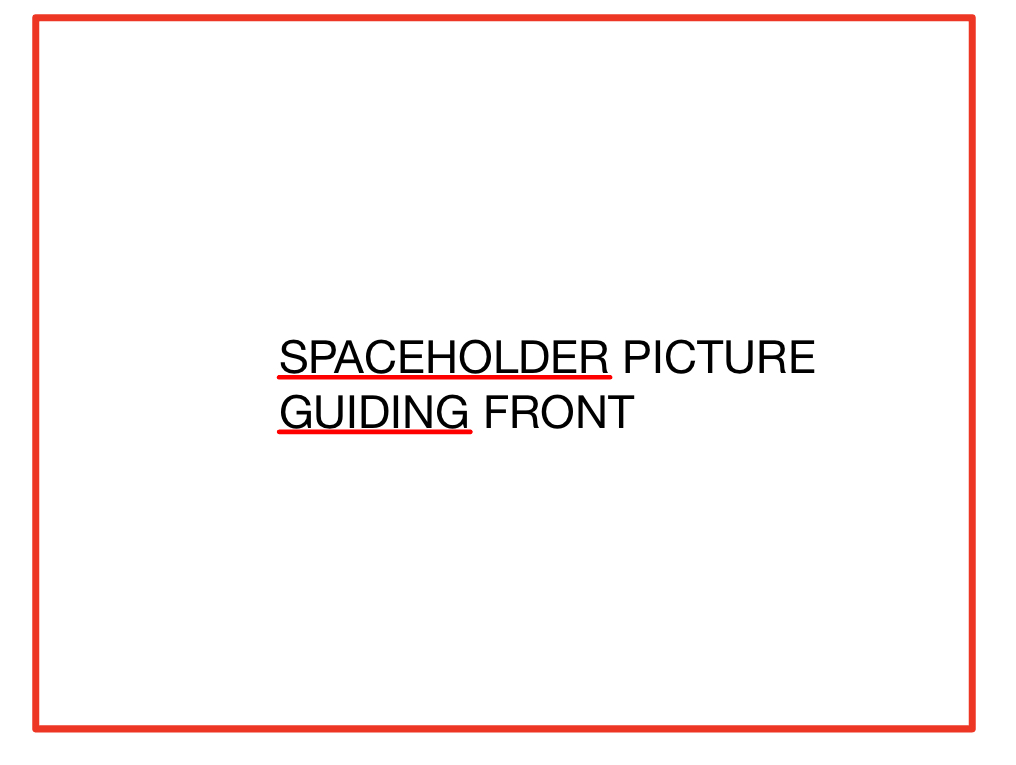
\includegraphics[width=\linewidth]{texfiles/mech/eimg/braking/guiding_front_1.jpg}
    \caption{CAD Guiding Front}
    \label{fig:guiding_front}
  \end{minipage}
  \hspace{0.5cm}
  \begin{minipage}[b]{0.45\linewidth}
    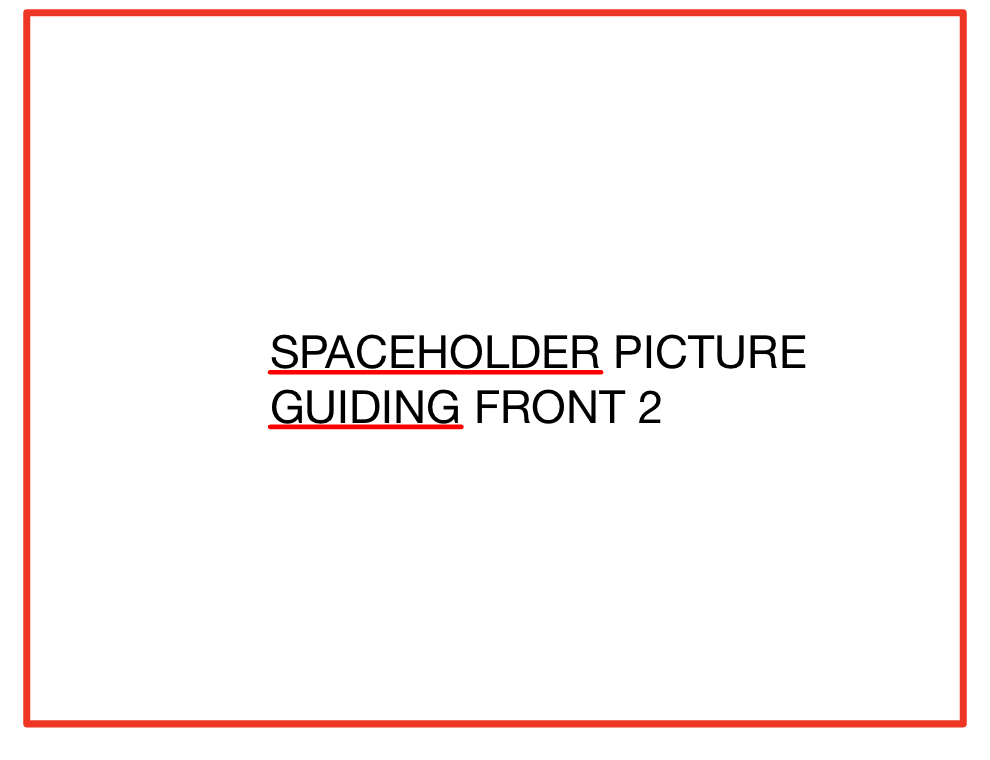
\includegraphics[width=\linewidth]{texfiles/mech/eimg/braking/guiding_front_2.jpg}
    \caption{CAD Guiding Rear}
    \label{fig:guiding_rear}
  \end{minipage}
\end{figure}

\begin{figure}[!ht]
  \centering
  \begin{minipage}[b]{0.45\linewidth}
    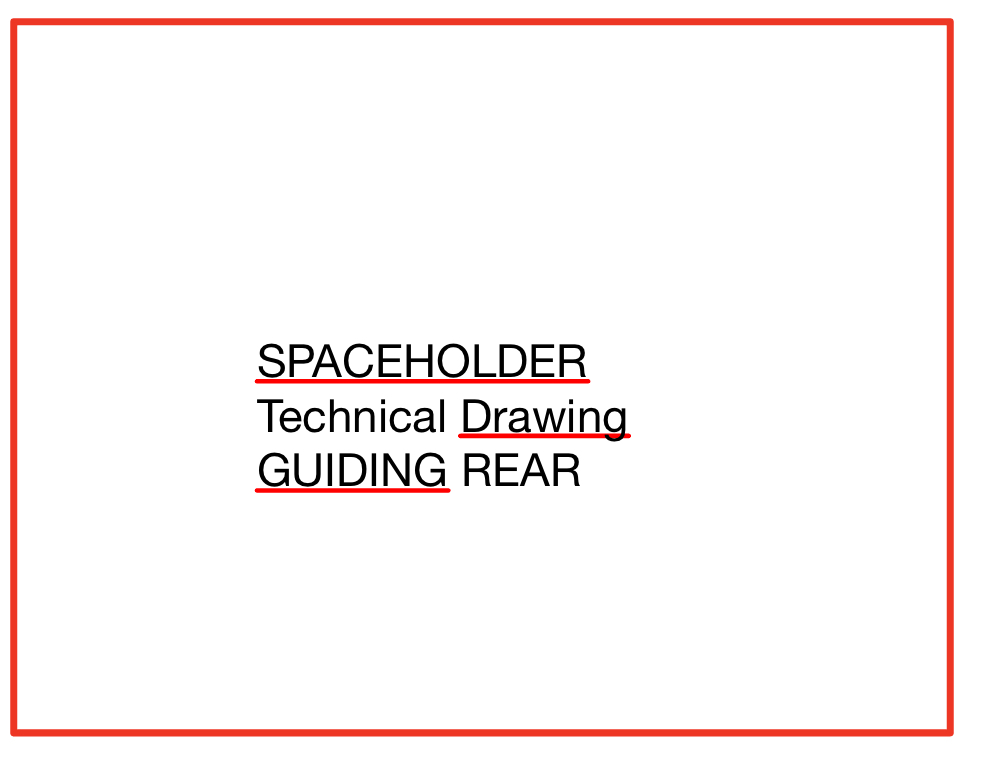
\includegraphics[width=\linewidth]{texfiles/mech/eimg/braking/guiding_tech_rear.jpg}
    \caption{CAD Guiding Front \#2}
    \label{fig:guiding_front_2}
  \end{minipage}
  \hspace{0.5cm}
  \begin{minipage}[b]{0.45\linewidth}
    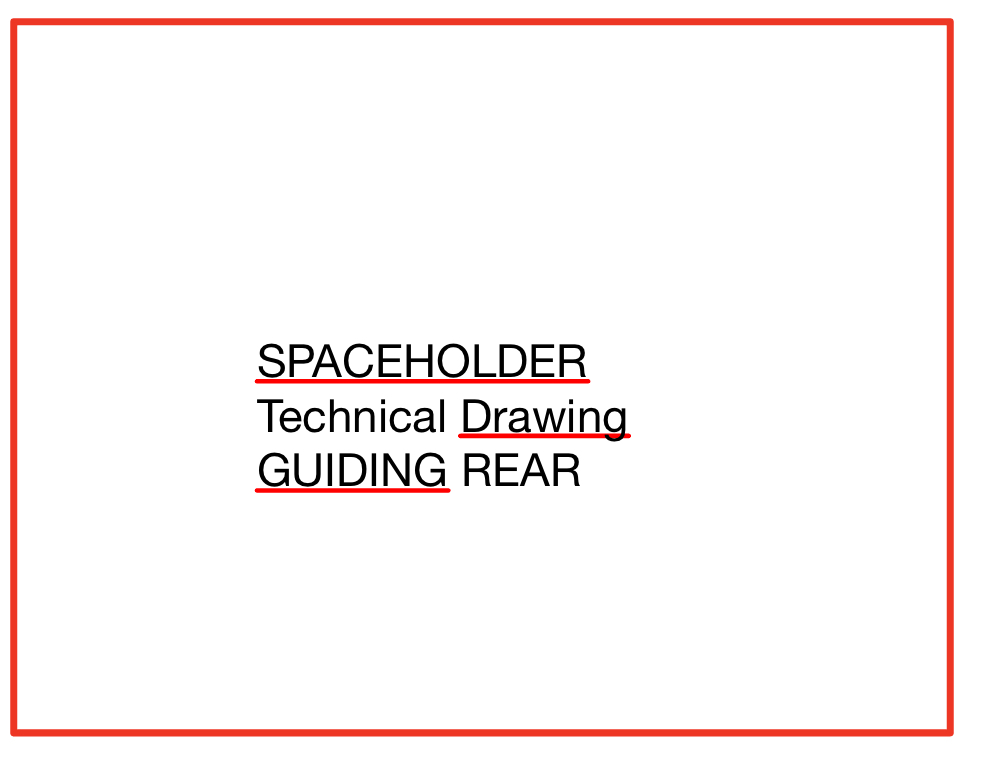
\includegraphics[width=\linewidth]{texfiles/mech/eimg/braking/guiding_tech_rear.jpg}
    \caption{CAD Guiding Rear 2}
    \label{fig:guiding_rear_2}
  \end{minipage}
\end{figure}

\begin{figure}[!ht]
  \centering
  \begin{minipage}[b]{0.45\linewidth}
    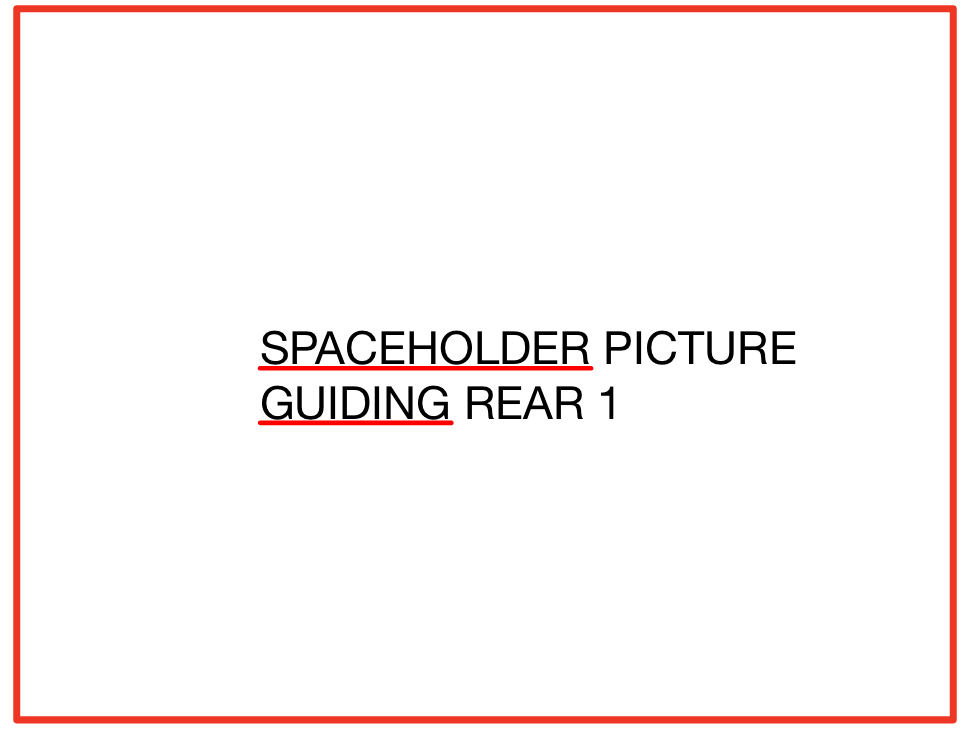
\includegraphics[width=\linewidth]{texfiles/mech/eimg/braking/guiding_rear_1.jpg}
    \caption{Technical Drawing Guiding Front }
    \label{fig:guiding_front_2}
  \end{minipage}
  \hspace{0.5cm}
  \begin{minipage}[b]{0.45\linewidth}
    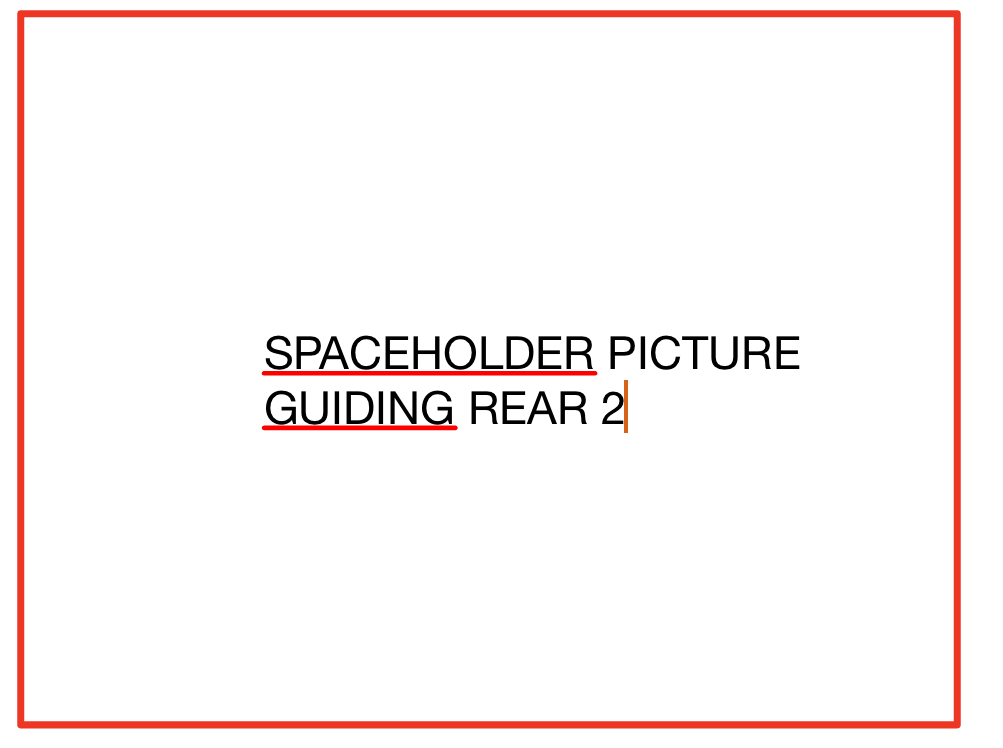
\includegraphics[width=\linewidth]{texfiles/mech/eimg/braking/guiding_rear_2.jpg}
    \caption{Technical Drawing  Guiding Rear}
    \label{fig:guiding_rear_2}
  \end{minipage}
\end{figure}

\newpage
\subsubsection{Materials}
To ensure maximum performance and longevity, the materials used for the subsystem components specifically, the small actuator mounting and the large brake mounting have been carefully chosen.  The choice of plain carbon steel can be attributed to its superior mechanical properties, affordability, and suitability for its intended application. It's also simple to work with and shape during production, which lowers costs and promotes efficient production.


Because plain carbon steel is durable and resistant to corrosion, it can withstand extreme conditions and last for a very long time. It is very easy to weld, which makes assembly simpler.

Finding the ideal mix between strength, the lifespan, ease of manufacture, and cost-effectiveness was the main consideration in the selection of plain carbon steel for these components.

\subsubsection{Design Rationale}
The main goal of the braking system design is to use advanced design ideas and make sure the pod can stop completely within predetermined parameters.

The design's fundamental idea is to use springs to provide a fail-safe mechanism. Our goal in using springs is to create a braking mechanism that can operate even in the case of a leak or system failure. The unique part is how the actuators are used to keep the springs compressed by operating in reverse. This design element strengthens the system's fail-safe capability by guaranteeing that the pod can activate braking even in the event of a malfunction or physical damage.
In conclusion, the braking system's creative use of actuators that operate in reverse and relying on springs are designed to promote safety and dependability. This method guarantees that even in difficult situations, the pod can brake within predefined limits. 
\subsubsection{FEM Results}
.  Present FEM results for worst-case scenarios, including images and values.
\paragraph{\Large{Calculations:}}






\begin{itemize}[leftmargin=*]
    \item[$\bullet$] \textbf{Kinetic Energy}
\end{itemize}

\noindent
For a pod with mass \(m=260\ \text{kg}\) and speed \(v=70\ \text{km/h}\), \textbf{kinetic energy} is defined as
\begin{align*}
    E_k &= \frac{1}{2} mv^2
\end{align*}
Substituting the given values:
\begin{align}
    E_k &= \mathbf{49151} \, \textbf{J}
\end{align}













\begin{itemize}[leftmargin=*]
  \item[\hspace{-1cm}$\bullet$] \textbf{Braking Force}
\end{itemize}
\noindent
To stop the pod within a certain distance, we must account for the work done to compensate for its kinetic energy. According to the principle of work, when an object moves against a force exerted on it, work is done. Specifically, if the object moves through a displacement $d$ while experiencing a constant force $F$, the force performs an amount of work given by




\[
W = F \cdot d
\]

To find the force \( F \) exerted on the pod, given that the work done is \( W = 49151~\text{J} \) and the stopping distance is \( d = 20~\text{m} \), we rearrange the formula:

\begin{align}
F &= \frac{W}{d} \notag \\
\textbf{Braking force } F &= \mathbf{2457.6}\, \textbf{N} 
\end{align}







\begin{itemize}[leftmargin=*]
    \item[$\bullet$] \textbf{Normal Force}
\end{itemize}
\noindent
To determine the required normal force exerted on the brake pads in order to achieve the necessary brake force, consideration must be given to the coefficient of friction ($\mu = 0.36$) between the brake pads and the track surface.






The required normal force (\( N \)) exerted on the brake pads can be calculated using the formula:

\begin{align}
    N &= \frac{F}{\mu} \notag \\     
  \textbf N  &= \mathbf{6826.66} \, \textbf{N}
\end{align}

where \( F = 2457.6 \) and \( \mu = 0.36 \).\\

The normal force per assembly, with consideration for two distinct assemblies, refers to the resultant force exerted perpendicular to the contact surfaces of each respective assembly.\\

\begin{equation}
\textbf{Normal force per assembly} = \mathbf{3413.28 \,N}
\end{equation}

\newpage
\begin{itemize}[leftmargin=*]
    \item[$\bullet$] \textbf{Spring Calculation}
\end{itemize}
\noindent
Given the parameters provided:

\begin{align*}
    \text{Resting length of the spring} (L_0) &= 187 \, \text{mm} \\
    \text{Spring constant} (k) &= 5.97 \, \text{N/mm} \\
    \text{Compressed length of the spring} (L_1) &= 94 \, \text{mm} \\
    \text{Actuator length} (L_{\text{actuator}}) &= 92 \, \text{mm} \\
    \text{Spring used in mounting} (L_{\text{mounting}}) &= 2 \, \text{mm}
\end{align*}
\noindent
When the spring is compressed from its resting length to the compressed length:

\begin{align*}
    \text{Initial Force} (F_{\text{initial}}) &= k \times (L_0 - L_1) \\
    &= 5.97 \times (187 - 94) \, \text{N} \\
    &= 555.21 \, \text{N}
\end{align*}
\noindent
Upon expansion of the spring to accommodate braking, extending to a length of 114 mm:

\begin{align*}
    \text{Force Required} (F_{\text{expansion}}) &= k \times (L_0 - L_{\text{braking}}) \\
    &= 5.97 \times (187 - 114) \, \text{N} \\
    &= 435.81 \, \text{N}
\end{align*}
\noindent
Since each assembly utilizes 8 springs, the total force required for both assemblies is:

\begin{equation}
\begin{aligned}
    \text{Total Force} (F_{\text{total}}) &= \text{Number of springs} \times F_{\text{expansion}}\notag \\
     \end{aligned}
\end{equation}
\begin{equation}
   \mathbf{Total\ Force} = \mathbf{6972.96 \, N}
\end{equation}



Considering the total normal force of 6826.66 N, it appears that the calculated force from the springs exceeds the total normal force, indicating that the system can function properly under these conditions.



\begin{itemize}[leftmargin=*]
    \item[$\bullet$] \textbf{Actuator Force}
\end{itemize}

\noindent
To determine if the chosen actuators can effectively compress and hold the springs to meet the normal force requirement, we need to calculate the total force capacity provided by all actuators. Given that we have 2 big actuators and 4 small actuators, each with a capacity of 686 N (at 6 bar pressure), we can calculate the total force capacity for each assembly:

\[
\textbf{Total force capacity} = \mathbf{4116} \, \textbf{N}
\]

Comparing this with the required normal force of 3413.28 N, we can see that the total force capacity provided by the actuators exceeds the requirement. Therefore, the chosen actuators are sufficient to compress and hold the springs to achieve the desired normal force on the track surface.

\newpage
\begin{itemize}[leftmargin=*]
    \item[$\bullet$] \textbf{Actuator Pressure}
\end{itemize}
\noindent
Given that the system can handle pressures between $6$ to $10$ bar, with $P_1 = 6$ bar and $F_1 = 686$ N (as per the catalogue) where the actuator can exert a force of $686$ N at $6$ bar.\\

With $8$ springs per assembly and a previously calculated compressed spring force of $555.21$ N, the total compressed spring force per assembly is $8 \times 555.21 = 4441.68$ N.\\
\noindent
Utilizing $6$ actuators per assembly, the required force from each actuator is 
\[
F_2 = 740.28 \, \text{N}.
\]

Now, let's calculate the pressure required for the actuators to handle this force: \\
 
- Using the formula $F = P \times A$, where $F_1 = P_1 \times A$ and $F_2 = P_2 \times A$.\\  
\[
P_2 = \frac{P_1 \times F_2}{F_1}.
\]  

- Substituting the given values, 
\begin{equation}
\mathbf{P_2} = \mathbf{6.47} \, \textbf{bar}.
\end{equation}

Hence, the pressure required for the actuators to handle this condition is approximately $6.5$ bar.
\subsubsection{Mesh and Boundary Conditions}
.  Provide details on the type of mesh, boundary conditions, and Free Body Diagrams.


\subsection{Manufacturing Process}
Kindly consult \textbf{Table \ref{table:components}} for reference.\\

\noindent
We've taken steps to ensure that our braking system is more than just a concept and can be manufactured realistically.\\

\noindent
\textbf{Selecting Materials Which Are Easy to Use}: The materials utilized for each component were selected based on their availability and convenience of production for the intended use. for instance, Carbon steel and other common metals, are chosen due to their easy production and wide availability.\\

\noindent
\textbf{Using Standard Parts}: We made an effort to use components that are widely available and simple to assemble, such as tubes, connectors, and adapters. As a result, producers can assemble everything more easily and without the need for specialized tools.\\ 

\noindent
\textbf{Assembly Ease}: The complete brake system's assembly has been taken into consideration. Parts are made to fit together easily, and assembly workers are assisted by clear labelling and instructions when needed.



\subsection{Integration process}
\subsubsection{Assembling}
Bolts will be used to firmly secure the main brake system to the chassis. Then, using specific mounts, small actuators will be fastened to the brake assembly.

Bolts will then be used to secure the aluminium brackets to the actuators. Before pressurizing the system, springs will be positioned between the metal brackets.




\subsubsection{Assembly interaction}
The longitudinal and lateral planes of the chassis must be securely fastened to the main mounting bracket. In in addition to providing structural support to the central section of the chassis, that connection will transmit forces to the chassis, resulting in the creation of a complete system.



\subsection{Safety Considerations}
\subsubsection{Safety Factor}
\textbf{Selecting Strong Materials:} Parts that make up pneumatic brakes, such as brake housings and valves, are made of hard materials such as steel and reinforced rubber These materials can withstand during braking.\\

\noindent
\textbf{To handle pressure safely:} Air brake systems operate under high pressure, so the parts are designed to handle much higher pressures than they will actually experience during normal use This additional capability this ensures that the system remains safe even if pressure fluctuations or screws occur.\\

\noindent
\textbf{Passing safety tests:} All parts in an air brake system go through rigorous tests to ensure they meet safety standards. These tests test things like how well the parts hold up under stress and whether they perform well under different conditions.\\

\noindent
\textbf{Backup system:} Many brake systems have a built-in backup system. For example, if one part fails, there is usually another part that can take over, ensuring that the brakes remain functional in an emergency. In our case, springs are used to create a brake mechanism that can operate even in the event of a leak or system failure. 
\subsubsection{Worst-Case Scenarios}

It can be dangerous to rely solely on air pressure in a standard pneumatic braking system without a fail-safe feature if the pressure drops unexpectedly or if there is a malfunction with the system.  \\

 \noindent
\textbf{Worst case scenario without Fail safe mechanism:}
This system only relies on air pressure. Leak of air or mechanical problem cause the air suddenly disappears, the brake might fail when needed. This makes accidents more likely.\\

\noindent
\textbf{Adding a Fail safe mechanism:}
if there is a problem with air pressure or  in case might be drop, this fail safe feature turns on by itself. it makes sure the brakes keep working even if pressure drop.

\subsection{FMEA Results Discussion}
\subsubsection{Risk Assessment}
.  Preliminary risk assessment for demonstration, transport, and lifting.
\subsubsection{FMEA and Risk Mitigation}
.  Detail FMEA and describe risk mitigation measures.
\subsubsection{Simulation Evidence}
.  Provide evidence of simulations validating theoretical assumptions.


\subsection{Testing}
\subsubsection{Safety Procedures Documentation}
Testing Procedures for Pneumatic Brake System\\

\noindent
\textbf{Pre-Test Inspection:}
Ensuring Braking component are properly attached and free from leaks.\\
Check that the compressed springs are at right place and working properly.\\

\noindent
\textbf{Pressure Check:} With use of pressure gauge to measure the air pressure in the system.\\
Continue increase the pressure to the recommended operating level and check for any pressure drops before operating system.\\

\noindent
\textbf{Monitor the expansion of the spring:}
Verify the expansion of spring as the air pressure decreases.Check that the spring works in Simultaneously with the actuator piston to maintain proper braking force.
Finally, Conduct a final inspection of all components of the system to ensure they remain in good condition.\\

\noindent
\textbf{Activate the Braking system by giving signal:}Check how actuator piston react and check that it moves forward correctly.
verify that the brake pad makes proper contact with the braking surface to create the friction that can enough to slow down the pod.\\

\noindent
\textbf{By applying emergency Brake Test:}
If we have to stop the vehicle in emergency situation,by conducting an emergency brake to check that it can able to quickly stop the pod. 

\subsubsection{Preliminary testing plan}
As we discussed above preliminary testing plan for the pneumatic braking system involves several key tests to validate its functionality and performance.\\
The expected results include regularly pressure build-up, smoother movement of piston, spring expansion and enough friction of brake pad to slow down the vehicle and  Safety precautions will be implemented throughout the testing process to ensure a safe environment and prevent any potential risk.

\subsection{Additional considerations}
\noindent
\subsubsection{Pneumatic Braking System:}
\paragraph{Possible Failures:} Brake systems can malfunction in a number of ways. it include malfunctioning , worn brake pads, pneumatic system failures, air leaks, worn brake pads or discs, electrical issues,  mechanical damage and weather conditions. Regular inspection and maintenance are essential to ensure the system's reliability and safety.
\paragraph{Pressure Requirement:}We are filling the pneumatic system with a pressure of 6.5 bar, well within the system's handling capacity, which ranges between 6 to 10 bar. To ensure that the pressure remains within safe limits, we are using a filling tank and pressure regulator. These components prevent the pressure from exceeding the specified limits and ensure the pneumatic system operates safely and effectively.\\
  
	
\subsection{References}
%Picture of Pneumatic Circuit


\section{Aerodynamics}


\subsection{Overview}
The design of the Hyperloop pod aeroshell is meticulously crafted to optimize aerodynamic performance and ensure stability during high-speed travel. This section explores the key design considerations and features of the aeroshell subsystem, highlighting its role in reducing air resistance and enhancing the overall efficiency of the Hyperloop transportation system.

\subsubsection{Requirements and Constraints}
The Hyperloop pod aeroshell is required to fulfill several critical functions to ensure optimal performance of the transportation system. Firstly, it must minimize air resistance to facilitate smooth movement through the Hyperloop tube, thereby reducing energy consumption and increasing overall speed. Additionally, the aeroshell should enhance stability and control during acceleration, deceleration, and maneuvers, contributing to passenger comfort and safety. Furthermore, the design should incorporate features to manage airflow efficiently, preventing turbulence and ensuring a streamlined flow around the pod. Compliance with safety regulations and structural integrity are also paramount, ensuring the aeroshell can withstand operational stresses and environmental conditions encountered during Hyperloop travel.

\subsubsection{Concept}
The concept of the aeroshell subsystem revolves around maximizing aerodynamic efficiency while ensuring structural integrity and safety compliance. Inspired by proven aerodynamic principles, the aeroshell design prioritizes minimizing air resistance, enhancing stability, and facilitating controlled airflow. By incorporating features such as a streamlined front and rear configurations, the aeroshell optimizes performance while maintaining adherence to safety standards and regulatory requirements outlined in the Functional Design Description (FDD) for the Hyperloop competition.
\subsubsection{Size, Components, and Appearance}
.  Include a table of materials, mass, dimensions, and other relevant factors.
\begin{table}[ht]
\centering

\label{table:components}
\begin{adjustbox}{width=\textwidth,center}
\begin{tabular}{|>{\bfseries}m{2.5cm}|m{1.4cm}|m{1.7cm}|m{2.1cm}|m{2.2cm}|m{2.6cm}|m{2.2cm}|}
\hline
Component & Number & Mass [kg] & Size [mm] & Material & Manufacturing process & In-house/ outsourced \\
\hline
Wheels & x8 & 1 & 100 x 50 & Polyurethane & Injection molding & Outsourced \\
Axles & x8 & 0.2 & 10 x 90 & Duplex Steel & Lathing & In-house \\
L-bracket 1 & x16 & 0.1 & 20x30x50 & Aluminium 7075 & Milling & In-house \\
L-bracket 2 & x8 & 0.2 & 30x40x60 & Aluminium 7075 & CNC & Outsourced \\
PART & AMOUNT & WEIGHT & SIZE & MATERIAL & PROCESS & SPONSORING \\
\hline

\end{tabular}
\end{adjustbox}
\caption{Components and Manufacturing Details}
\end{table}


\subsection{Theoretical concepts}

Theoretical understanding forms the backbone of our approach towards designing the aerodynamic components of the Hyperloop pod. In this section, we delve into the foundational concepts guiding our Computational Fluid Dynamics (CFD) simulations, specifically focusing on the utilization of the \(k-\omega\) SST turbulence model.

\subsubsection{Relevance of Turbulence Modeling}

Turbulence plays a pivotal role in determining the flow characteristics around the Hyperloop pod as it travels through the tube. Traditional approaches relying solely on laminar flow assumptions are inadequate for capturing the complex flow phenomena at high speeds encountered in the Hyperloop environment. Therefore, turbulence modeling becomes indispensable for accurately predicting flow behavior, including boundary layer separation, vortex shedding, and wake formation.

\subsubsection{Introduction to \(k-\omega\) SST Turbulence Model}

The \(k-\omega\) SST (Shear-Stress Transport) turbulence model is a widely used approach in CFD simulations, renowned for its robustness and accuracy in capturing both near-wall and free-stream turbulence effects. This model combines the strengths of the \(k-\omega\) and \(k-\epsilon\) models, making it suitable for simulating a wide range of flow regimes, from boundary layers to separated flows.

\subsubsection{Key Features of \(k-\omega\) SST Model}

The \(k-\omega\) SST model resolves turbulent viscosity through two transport equations: one for turbulent kinetic energy (\(k\)) and the other for specific turbulence dissipation rate (\(\omega\)). By incorporating wall functions and a low-Reynolds number correction, this model accurately predicts near-wall behavior while maintaining stability and computational efficiency. Additionally, the SST formulation seamlessly transitions between the near-wall region, where wall functions are utilized, and the outer flow region, where the standard \(k-\omega\) model is applied.

The equations governing the \(k-\omega\) SST model are as follows:

\begin{align*}
\frac{\partial (\rho k)}{\partial t} + \frac{\partial (\rho u_j k)}{\partial x_j} &= P_k - \beta^* \rho \omega k + \frac{\partial}{\partial x_j} \left[ \left( \mu + \frac{\mu_t}{\sigma_k} \right) \frac{\partial k}{\partial x_j} \right] \\
\frac{\partial (\rho \omega)}{\partial t} + \frac{\partial (\rho u_j \omega)}{\partial x_j} &= P_\omega - \beta \rho \omega^2 + \frac{\partial}{\partial x_j} \left[ \left( \mu + \frac{\mu_t}{\sigma_\omega} \right) \frac{\partial \omega}{\partial x_j} \right]
\end{align*}

where:
\begin{itemize}
    \item \(P_k\) and \(P_\omega\) are the production terms for \(k\) and \(\omega\) respectively,
    \item \(\beta\) and \(\beta^*\) are constants,
    \item \(\mu\) is the dynamic viscosity,
    \item \(\mu_t\) is the turbulent viscosity,
    \item \(\sigma_k\) and \(\sigma_\omega\) are the turbulent Prandtl numbers.
\end{itemize}

\subsubsection{Aerodynamics Concepts: Lift and Drag}

In aerodynamics, lift and drag are two fundamental forces that influence the motion of an object through a fluid. Lift is the force perpendicular to the relative motion of the fluid and the object, while drag is the force parallel to the relative motion.

The lift force (\(L\)) and drag force (\(D\)) can be calculated using the following formulas:

\begin{align*}
L &= \frac{1}{2} \rho V^2 S C_L \\
D &= \frac{1}{2} \rho V^2 S C_D
\end{align*}

where:
\begin{itemize}
    \item \(\rho\) is the fluid density,
    \item \(V\) is the velocity of the flow relative to the object,
    \item \(S\) is the reference area (such as wing area for an airfoil),
    \item \(C_L\) is the lift coefficient,
    \item \(C_D\) is the drag coefficient.
\end{itemize}

\subsubsection{Key Fluid Mechanics Concepts}

Several key principles from fluid mechanics are crucial for understanding aerodynamic behavior in CFD simulations:

\begin{itemize}
    \item \textbf{Reynolds Number (\(Re\))}: A dimensionless quantity representing the ratio of inertial forces to viscous forces in the flow. It is defined as \(Re = \frac{\rho V L}{\mu}\), where \(\rho\) is the fluid density, \(V\) is the velocity, \(L\) is a characteristic length (such as chord length for an airfoil), and \(\mu\) is the dynamic viscosity.
    
    \item \textbf{Boundary Layer}: The thin layer of fluid adjacent to the surface of an object where viscous effects dominate. Understanding boundary layer behavior is essential for predicting aerodynamic drag and lift forces accurately.
    
    \item \textbf{Turbulent Flow}: Flow characterized by chaotic, irregular motion with fluctuations in velocity and pressure. Turbulent flow phenomena significantly affect drag, lift, and heat transfer in aerodynamic systems.
\end{itemize}
\subsubsection{Unique Flow Regime}

The Hyperloop pod operates within a distinctive flow regime characterized by very low Reynolds numbers (\(Re\)) and high Mach numbers (\(Ma\)). At low Reynolds numbers (\(Re < 10^6\)), viscous effects dominate, resulting in laminar flow over most of the aeroshell surface. High Mach numbers (\(Ma > 0.3\)) introduce compressibility effects, necessitating careful consideration of shock wave formation and drag rise. The interplay between these factors significantly influences the aerodynamic performance of the pod.

\subsubsection{Boundary Layer Control}

Effective boundary layer control is paramount for optimizing the aerodynamic efficiency of the pod. Transition delay techniques, such as passive and active boundary layer control, are employed to mitigate boundary layer separation and delay the onset of turbulent flow. Shaping the aeroshell to promote laminar-to-turbulent transition further upstream helps maintain attached flow and reduce drag. Additionally, employing boundary layer suction or blowing can manipulate flow separation points, enhancing overall aerodynamic performance.

\subsubsection{Kantrowitz Limit}

The Kantrowitz limit poses a critical challenge in the design of the Hyperloop pod aeroshell. Near this limit, where the pod's diameter approaches half the diameter of the tube, compressibility effects become significant. As the pod approaches transonic speeds, shock waves form, leading to increased drag and potential instability. Mitigating the adverse effects of the Kantrowitz limit requires careful shaping of the aeroshell to minimize wave drag and reduce perturbations in the flow field.



\subsubsection{Meshing in CFD Simulations}

Meshing, or grid generation, is a crucial step in CFD simulations that involves dividing the computational domain into discrete elements or cells. A well-structured mesh ensures accurate representation of flow physics while minimizing computational cost. For our Hyperloop pod simulations, a structured meshing approach is adopted to ensure optimal grid quality and resolution in critical flow regions.

\subsubsection{Finite Element Method (FEM)}

The Finite Element Method (FEM) is a numerical technique used to solve partial differential equations governing physical phenomena, such as fluid flow and structural mechanics. In the context of CFD simulations, FEM is employed to discretize the governing equations over the computational domain, enabling the solution of complex fluid flow problems. By dividing the domain into finite elements and employing appropriate interpolation functions, FEM facilitates the accurate approximation of flow variables within each element.

\subsubsection{Integration into CFD Simulations}

For our Hyperloop pod design, the \(k-\omega\) SST turbulence model serves as a cornerstone in our CFD simulations. By accurately capturing turbulent flow phenomena, including laminar-to-turbulent transition
\subsection{Results of Simulations}
\subsubsection{CFD Simulations}
\subsubsection{FEM Simulations}


(To be done)The results of computational fluid dynamics (CFD) simulations provide valuable insights into the aerodynamic behavior of the Hyperloop pod aeroshell. Detailed analysis of flow patterns, pressure distributions, and drag coefficients derived from simulations inform design refinements and performance enhancements. The following subsection presents key findings and observations obtained from CFD simulations conducted on the Hyperloop pod aeroshell design.

\subsection{Design Process and Appearance}
\subsubsection{CAD Models and Technical Drawings}
.  Present CAD models and technical drawings.
\begin{figure}[!ht]
  \centering
  \begin{minipage}[b]{0.45\linewidth}
    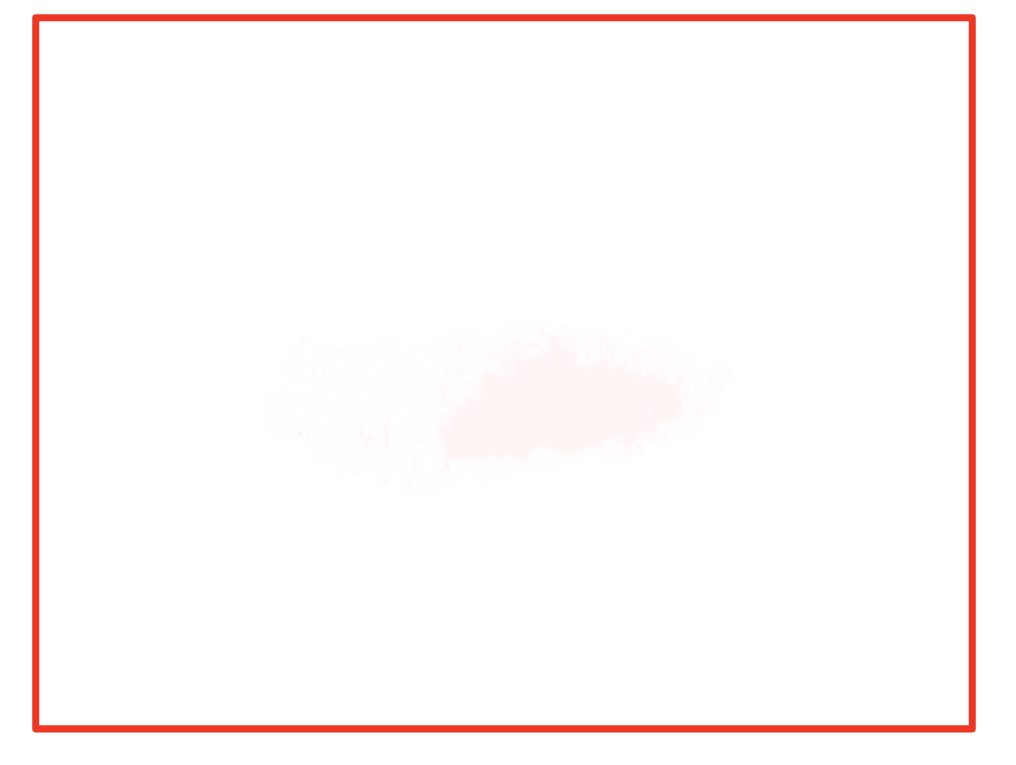
\includegraphics[width=\linewidth]{texfiles/mech/eimg/aerodynamics/shell_frontview}
    \caption{CAD shell Frontview}
    \label{fig:shell_frontview}
  \end{minipage}
  \hspace{0.5cm}
  \begin{minipage}[b]{0.45\linewidth}
    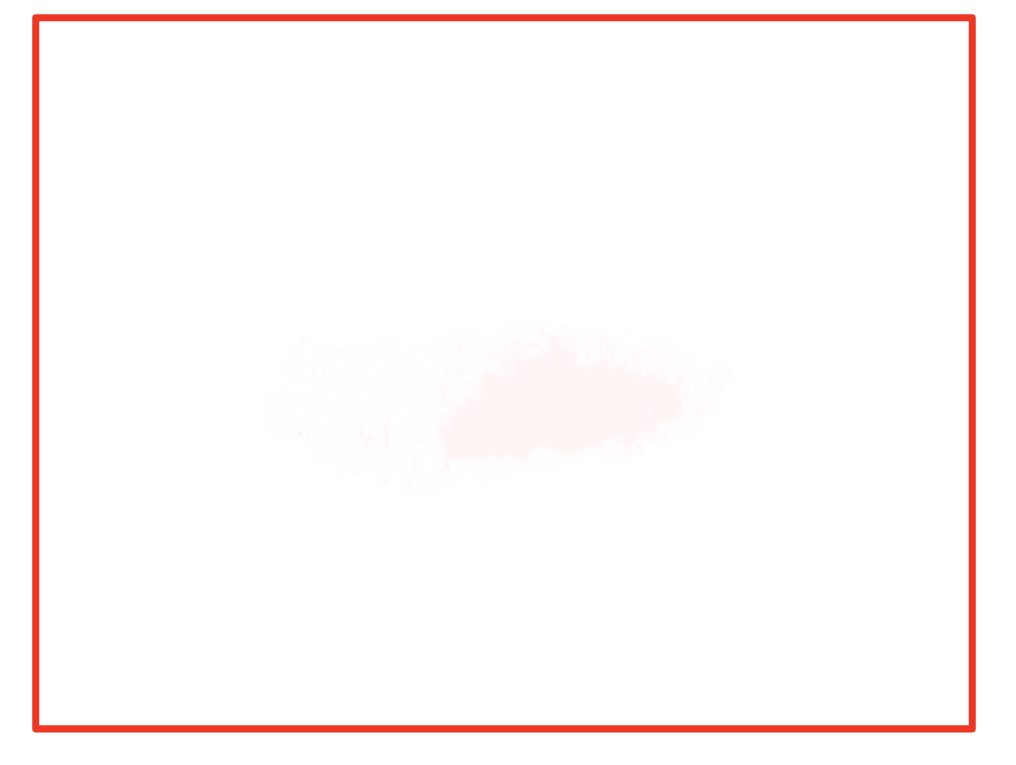
\includegraphics[width=\linewidth]{texfiles/mech/eimg/aerodynamics/shell_side}
    \caption{CAD shell sideview}
    \label{fig:shell_sideview}
  \end{minipage}
\end{figure}

\begin{figure}[!ht]
  \centering
  \begin{minipage}[b]{0.45\linewidth}
    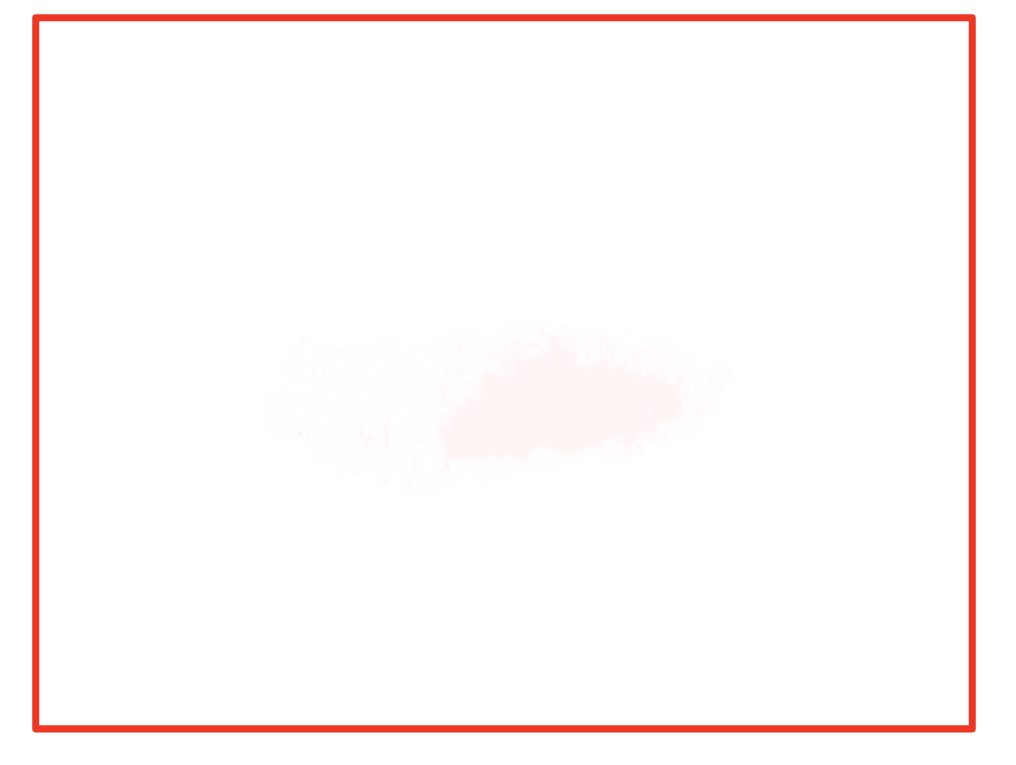
\includegraphics[width=\linewidth]{texfiles/mech/eimg/aerodynamics/shell_rear}
    \caption{CAD Shell back}
    \label{fig:shell_back}
  \end{minipage}
  \hspace{0.5cm}
  \begin{minipage}[b]{0.45\linewidth}
    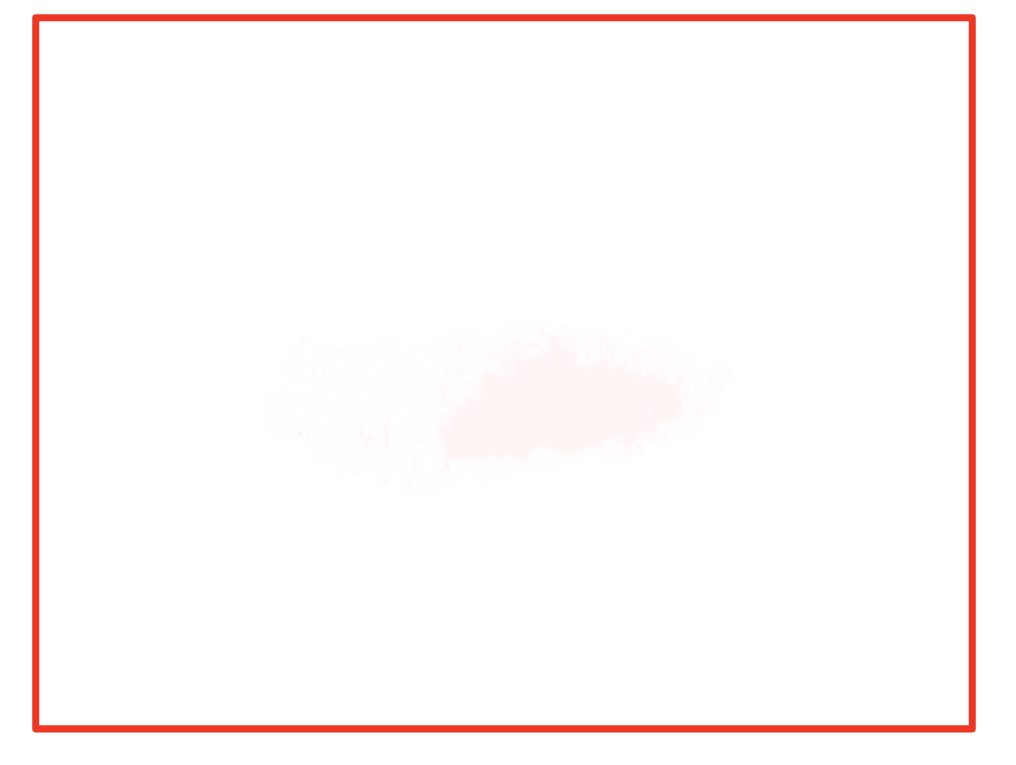
\includegraphics[width=\linewidth]{texfiles/mech/eimg/aerodynamics/shell_topview}
    \caption{CAD shell topview}
    \label{fig:shell_topview}
  \end{minipage}
\end{figure}

\begin{figure}[!ht]
  \centering
  \begin{minipage}[b]{0.45\linewidth}
    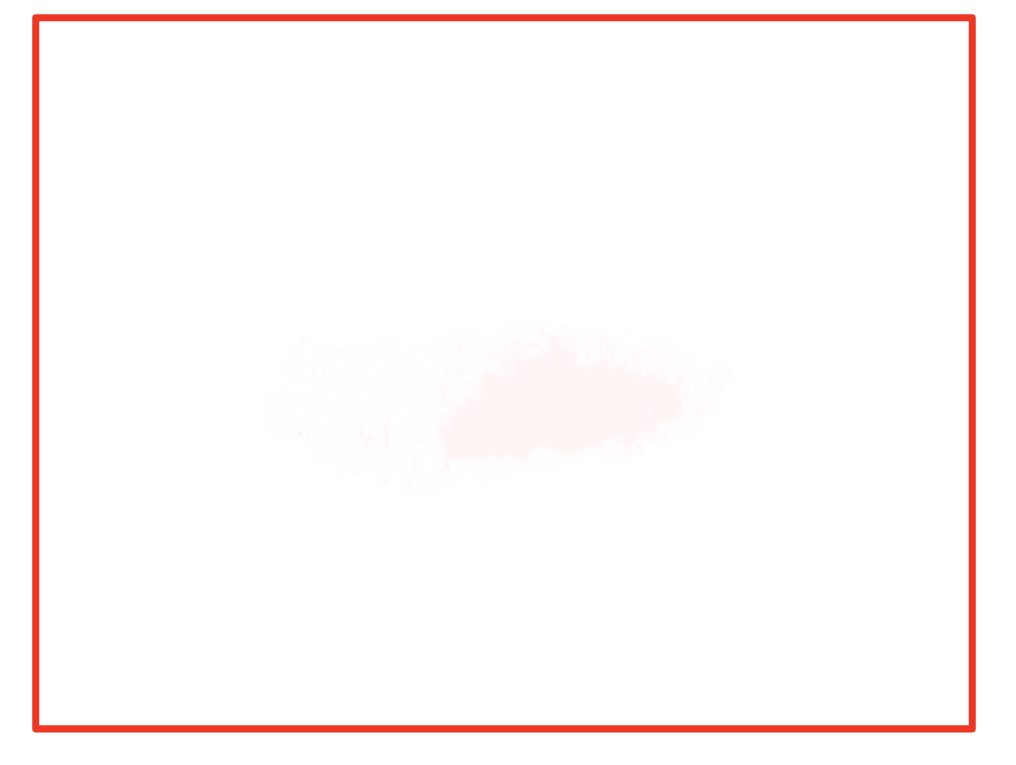
\includegraphics[width=\linewidth]{texfiles/mech/eimg/aerodynamics/shell_drawing}
    \caption{CAD Shell drawing }
    \label{fig:shell_drawing}
  \end{minipage}
  \hspace{0.5cm}
  \begin{minipage}[b]{0.45\linewidth}
    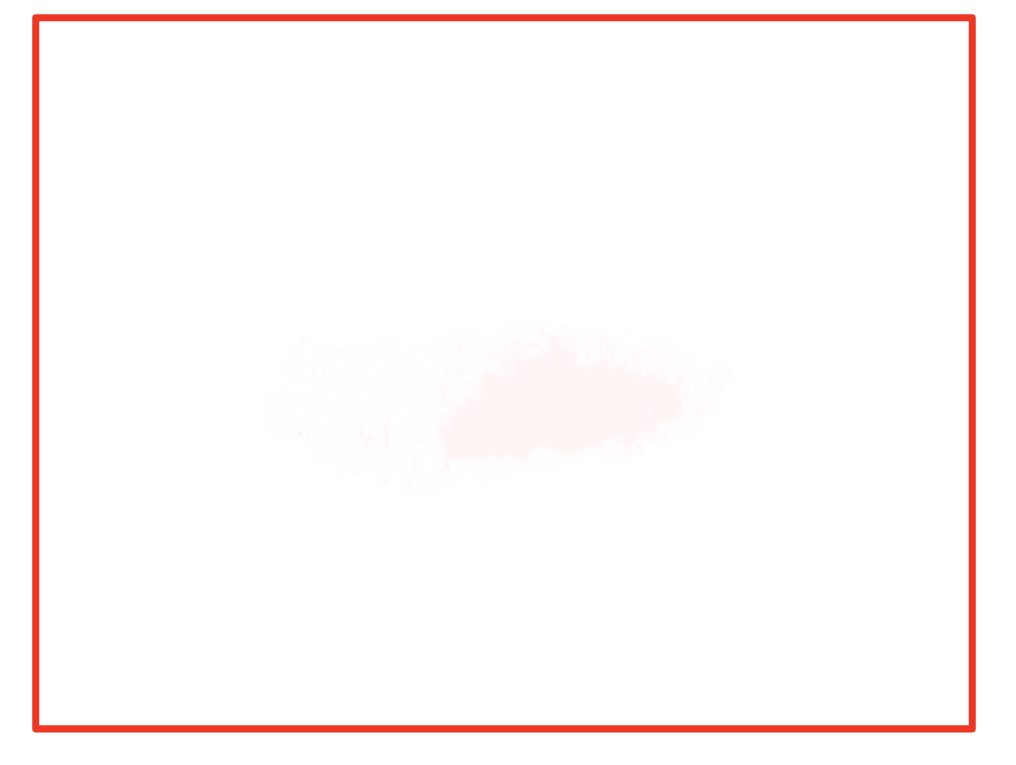
\includegraphics[width=\linewidth]{texfiles/mech/eimg/aerodynamics/shell_bottom}
    \caption{CAD shell bottom}
    \label{fig:shell_bottom}
  \end{minipage}
\end{figure}
\par %

\subsubsection{Materials}
.  Present and justify the selection of materials used in the subsystem
.  Provide relevant properties of the materials selected.
The Aeroshell is constructed sustainably with natural basalt fibre for biodegradability and superior tensile strenth. This iteration we used 3D printes molds, which enhance the design precision. Furthermore various safety features have been added to the Body, including using Polyester based Resins that are fire resistant.
\par %

\subsubsection{Design Rationale}
.  Detail the design rationale behind the components of the infrastructure.
.  Provide a rationale for why the specific configuration has been chosen
\newline
The Hyperloop shell was designed in Autodesk Fusion 360. First we collected several information about optimal aerodynamic shell designs.To fit the chassis we went with a rounded rectangular form. The shell has smooth and regular surfaces for laminar airflow. Originally doors were planned for easy access to the battery. Due to time constraints we decided to implement a quick release mechanism so one is able to “take off” the whole shell and have access to the whole chassis. Furthermore the rear end is flattened to reduce the drag force on our pod.
\par %


\subsubsection{FEM Results}
.  Present FEM results for worst-case scenarios, including images and values.
\paragraph{Calculations}
.  Provide reasoning and the necessary calculations to justify the simulated loads.
\subsubsection{Mesh and Boundary Conditions}
.  Provide details on the type of mesh, boundary conditions, and Free Body Diagrams.


\subsection{Manufacturing Process}
.  Compile a parts list in tabular format, specifying in-house or outsourced production.
.Describe what efforts have been made so that the designed part is realistically manufacturable.
\begin{table}[ht]
\centering

\label{table:components}
\begin{adjustbox}{width=\textwidth,center}
\begin{tabular}{|>{\bfseries}m{2.5cm}|m{1.4cm}|m{1.7cm}|m{2.1cm}|m{2.2cm}|m{2.6cm}|m{2.2cm}|}
\hline
Component & Number & Mass [kg] & Size [mm] & Material & Manufacturing process & In-house/ outsourced \\
\hline
Bed lift & x2 & 7 & - & steel & - & Outsourced \\
Lamination bolt & x8 & 0,01 & M6 & stainless steel & - & Outsourced \\
Nuts & x8 & 0,0012 & M6 & alloyed steel & - & Outsourced \\
3D-Print & x1 & - & - & - & - & Outsourced \\
Epoxidharz & x1 & - & - & - & -& Outsorced \\
PART & AMOUNT & WEIGHT & SIZE & MATERIAL & PROCESS & SPONSORING \\
\hline

\end{tabular}
\end{adjustbox}
\caption{Components and Manufacturing Details}
\end{table}

\par %

The construction process for Fermions aeroshell involves a systematic approach to ensure the optimal integration of basalt fibers and polyester resin. Beginning with a detailed design and 3D model, the chosen shape, dimensions, and structural requirements are meticulously defined using Autodesk Fusion 360. To get the shape designed in CAD, we are 3D-printing our Shell. Following material selection a custom mold is prepared to reflect the rounded rectangular aeroshell geometry. \newline
In preparation for the layup process, the mold undergoes surface treatment with a mold release agent to facilitate subsequent removal. Basalt fibers are then cut to specified lengths and strategically laid onto the mold, ensuring even distribution and coverage, particularly in areas with complex shapes or anticipated high-stress points. The wet layup method is employed, involving the careful application of polyester resin to saturate and bond with the basalt fibers. \newline
To consolidate the composite structure, a consolidation tool is utilized, eliminating air bubbles and enhancing the adhesion between the basalt fibers and the resin. The aeroshell is left to fully dry. Following a thorough curing process, the aeroshell is demolded with precision to prevent damage to the composite structure. \newline
Post-demolding, excess material is trimmed, and meticulous finishing is conducted to achieve a smooth and aerodynamic surface. After the shell is cured and demoulded, the mountings will be fixed from the inside with layup. To give Fermion a modern look and therefore visualize the new and futuristic approach of the hyperloop system, the shell will be painted. \newline

\subsection{Integration process}
\subsubsection{Assembling}
\textbf{Preparation Phase:} 
Firstly, we gather all the necessary components, such as the aeroshell, chassis, and lifting mechanism. We meticulously inspect each part, ensuring they're in optimal condition for assembly. If we spot any damaged or faulty components, we promptly replace them to avoid any issues during integration.

\textbf{Assembly of Lifting Mechanism:} 
Following the preparation phase, we carefully assemble the lifting mechanism according to the manufacturer's instructions. This involves constructing the hydraulic arms and triangular metal structure. Proper assembly is crucial for the smooth operation and safety of the lifting process.

\textbf{Attachment to Chassis:} 
Once the lifting mechanism is assembled, we securely attach it to the chassis. We make sure to create a firm and stable connection to support the weight of the aeroshell during lifting. Bolting the lifting mechanism securely to the chassis is vital for stability and safety.
\subsubsection{Assembly interaction}
\textbf{Lifting the Aeroshell:} 
With the lifting mechanism securely in place, we begin the process of lifting the aeroshell. We lift it evenly and cautiously to prevent any tilting or imbalance that could potentially damage the aeroshell. Careful operation of the lifting mechanism is essential for a safe and smooth lifting process.

\textbf{Integration Phase:} 
Once the aeroshell is lifted to the appropriate height, we carefully lower it onto the chassis. Alignment is critical at this stage to ensure proper fitting and performance. We verify that the aeroshell aligns correctly with the mounting points on the chassis.

\textbf{Securing and Final Checks:} 
After positioning the aeroshell on the chassis, we secure it using appropriate fasteners. We ensure these fasteners are tightened securely to firmly attach the aeroshell to the chassis. Conducting a thorough final inspection is crucial to confirm the secure attachment of the aeroshell and the proper functioning of the lifting mechanism.

\textbf{Final Checks:} 
In the final stage of the integration process, we conduct a comprehensive inspection. We check to ensure that the aeroshell is securely attached and that the lifting mechanism is functioning correctly. Any issues identified during these final checks are addressed promptly to ensure successful integration.



\subsection{Safety Considerations}
\subsubsection{Safety Factor}
.  Discuss the safety factor applied to structural elements.
\par %
Various safety measures have been considered to minimize failures. Furthermore performing FEA ensures that our aeroshell can sustain High Shear Stresses. An assembly test was performed to ensure violation of the keep out zones. As already mentioned in "Materials", the resins for the chosen composite are fire resistant.
\par %
\subsubsection{Worst-Case Scenarios}
.  Discuss worst-case scenarios (e.g., worst-case braking deceleration) and what you plan to do to avoid or contain them.
\par %
1. Structural Failure: 
\par %
Structural fatigue could result from manufacturing defects, material weaknesses or unforeseen stress factors. To avoid structural failure, we carefully selected materials with high fatigue resistance for constructing the aeroshell. (carbon fiber reinforced polymers)
\par %
2. High speed collision:
\par %
High speed collisions could occur when external objects penetrate the shell. The Aeroshell must be able to withstand the impact forces. Similar to the first point, we are using carefully selected materials.
\par %
3. Fire Incidents:
\par %
In the event of a fire within the system, the aeroshell ist designed to withstand high temperatures and prevent the spread of flames due to the fire resistant resins.
\par %
\subsection{FMEA Results Discussion}
\subsubsection{Risk Assessment}
.  Preliminary risk assessment for demonstration, transport, and lifting.
\subsubsection{FMEA and Risk Mitigation}
.  Detail FMEA and describe risk mitigation measures.
\subsubsection{Simulation Evidence}
.  Provide evidence of simulations validating theoretical assumptions.


\subsection{Testing}
\subsubsection{Safety Procedures Documentation}
.  Describe testing procedures.
\subsubsection{preliminary testing plan}
.  Provide a preliminary testing plan, including methodology and expected results.


\subsection{Additional considerations}
.  Additional considerations when writing the document for specific subsystems: Breaking, Pneumatic system, Aeroshell.
i. 		Include CFD analyses for the conditions expected during the demonstration, and their
		results, covering values such as lift, drag, or moment coefficient.
ii. 		If you plan on demonstrating inside a tube, include it in the CFD simulations.
iii. 	In case the system uses high voltage, indicate how will the MIDs be shut off when the
		aeroshell is covering the pod



\section{Cooling System} 
\subsection{Overview}
\subsubsection{Requirements and Constraints}
The cooling system plays a pivotal role in keeping the motor, battery, and traction controller within safe temperature limits. Overheating can lead to reduced efficiency and potentially shorten the lifespan of these components. For instance, excessive heat could cause bearings to wear out faster, damage motor windings, and even demagnetize permanent magnets. Given the hyperloop's low-pressure environment, we must think beyond standard air cooling methods. Consequently, the exploration of alternative cooling techniques, such as liquid cooling, cooling with the Phase Changing Materials are becoming imperative for ensuring the system's reliability and efficiency.

\subsubsection{Estimated Cost and Part List}
The total estimated manufacturing cost for the cooling system is approximately 1200 Euros, considering the primary components outlined in the table. Despite its comprehensive functionality, the system maintains a relatively lightweight and compact profile, comprising only a select few components. This cost-effective design approach ensures efficient performance without compromising on reliability or functionality.


\autoref{table:components}
\begin{table} [H]
\centering
\caption{Components and Manufacturing Details}
\label{table:components}
\begin{adjustbox}{width=\textwidth,center}
\begin{tabular}{|>{\bfseries}m{2.9cm}|m{2.4cm}|m{1.7cm}|m{2.5cm}|m{2.2cm}|m{2.6cm}|m{2.2cm}|}
\hline
Component & Number & Mass [kg] & Size [mm] & Material & Manufacturing process & In-house/ Outsourced \\
\hline
Heat Exchanger & x1 & 1.1 & 100 x120 x100 & Aluminum & LPBF Printing & in-house \\
Drain Valve & x1 & 0.02 & M8 & Aluminum & Latheturning & in-house \\
PCM & x1.75 [liters] & 2 & - & PCM & - & outsourced \\
Deionized Water & x3 [liters] & 3 & - & Water & - & outsourced \\
Coolant Pump & x1 &1.2 & - & - & - & outsourced \\
Filter &x1 & 0.1 & - & - & - &outsourced \\
Coolant Temperature Sensor & x2 & 0.2 & - & - & - & outsourced \\
Surface Temperature Sensor & x3 & 0.2 & - & - & - & outsourced \\
Flow Meter & x1 & 0.1 & - & - & - & outsourced \\
Pressure Sensor & x4 & 0.1 & - & - & - & outsourced \\
Piping & x5 [meters] & 0.9 &  10 x 16& - & - & outsourced \\
Piping & x2 [meters] & 0.4 & 20 x 26 & - & - & outsourced \\
Tank & x1 & 0.2 & 138 x 160 & - & - & outsourced \\

Fittings & x15 & - & - & - & - & outsourced \\
\hline
\end{tabular}
\end{adjustbox}
\end{table}


\subsection{Objectives, Design process, and Cooling Requirements}
\autoref{fig:Cooling system}
\begin{figure}[ht]
  \centering
  \subfloat[Front view of the pod]{
    \centering
    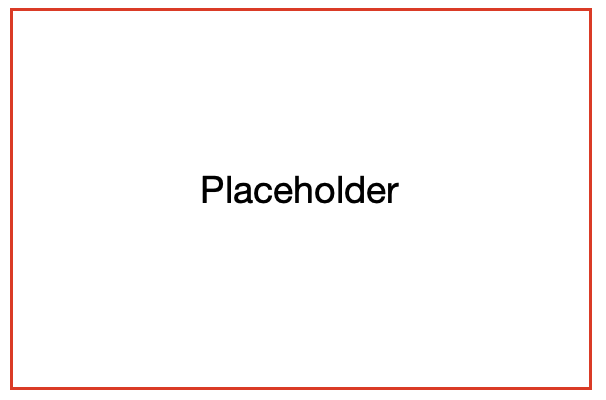
\includegraphics[width=0.5\linewidth]{texfiles/mech/eimg/cooling/placeholder}
    \label{fig:Front view}
  }
  \subfloat[Top view of the pod]{
    \centering
    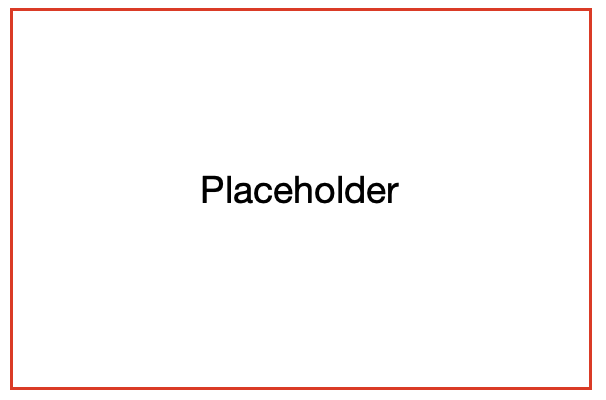
\includegraphics[width=0.5\linewidth]{texfiles/mech/eimg/cooling/placeholder}
    \label{fig:Top view}
  }
  \caption{Placement of the Cooling system}
  \label{fig:Cooling system}
\end{figure}


\subsubsection{ Motor}
The EMRAX motor is required to operate within a temperature range of -40°C to 120°C for both the copper windings and magnets. To safeguard against overload, a temperature sensor is integrated into the motor and must be linked to the controller. If the temperature surpasses the permissible limit, the controller adjusts the motor's current output to lower levels until the temperature stabilise within the acceptable range, with a worst-case motor efficiency of 92\%, approximately 4.8 kW of heat is generated during operation.

The manufacturer recommends a coolant flow rate of 6 to 8 litres per minute, with the coolant maintained at a maximum temperature of 50°C when entering the motor. Additionally, ambient air temperature surrounding the motor should ideally be 25°C or lower. [Ref - Product Spec Emrax Motor]


\subsubsection{ Traction Controller}

According to the product specification, the maximum permissible temperature for the traction controller is 150°C. However, to guarantee peak performance and longevity, it's essential to maintain temperatures below 90°C. After assessing the operating current and internal resistance, the estimated heat generation was calculated to be 0.56 kW. Through heat transfer calculations from the power module baseplate, equipped with fins, to the coolant, a water flow rate of 0.7 litres per minute was determined necessary to sustain the traction controller's temperature at 90°C.This ensures optimal cooling performance and contributes to the longevity and efficiency of the entire cooling system.
\subsubsection{ Battery}
The battery system within the hyperloop pod generates approximately 3.84 kW of heat during operation. This heat generation is primarily due to internal resistance within the battery cells as electrical energy is converted into usable power. To maintain safe and efficient operation, it is imperative to ensure that the temperature of the battery remains below 75°C.

When a battery operates at elevated temperatures, several detrimental effects may occur. High temperatures can accelerate the degradation of battery components, including the electrolyte and electrode materials, leading to reduced battery capacity and lifespan. Additionally, overheating increases the risk of thermal runaway, a phenomenon where the battery temperature rapidly increases, potentially resulting in fire or explosion.


\subsubsection{Cooling Requirements and Strategies}
To mitigate these risks and ensure the longevity and safety of the battery system, effective cooling strategies are essential. This includes implementing cooling systems, such as liquid cooling or cooling plates, to dissipate the heat generated by the battery during operation.

To ensure optimal cooling for all three vital components, the system necessitates a total coolant volume of 1 liters of de-ionised water. This calculation factors in the total heat generation (9.2 kW), the duration of a single run at the European Hyperloop Week Competition (20 seconds), and a safety factor of 3 (total time 60 seconds). After 60 seconds of operation, the maximum temperature of the 3 liters of coolant reaches approximately 66.5°C, well below the specified temperature limits. Further analysis during testing phase will provide valuable insights into coolant temperature changes and component temperatures.

To enhance the cooling performance of the cooling System, a refined hardware architecture will be implemented. Temperature levels play a critical role in determining the durability and efficiency of the motor, battery, and traction controller within the hyperloop pod. Elevated temperatures can adversely affect various components, including bearings, motor windings, and permanent magnets, potentially leading to demagnetisation. Therefore, prioritising the enhancement of cooling systems is essential for achieving significant long-term cost savings and improved performance. Given the impracticality of air cooling in the low-pressure hyperloop tube environment, alternative approaches such as liquid cooling and the use of Phase changing materials must be explored.

\subsubsection{Hardware Architecture for Enhanced Cooling}

As illustrated in  figure ~\ref{fig:schematic}, cold water stored at room temperature (approximately 20-25°C) will undergo filtration and then be pumped into the water jackets of the motor, traction controller, and battery in a closed-loop configuration, with a flow rate ranging from 8 to 12 liters per minute. Continuous monitoring of the coolant, motor, traction controller, and battery temperatures will be conducted. Should the temperature of any component exceed the specified limit, the control system will promptly deactivate the pod's drive motor.

Given the absence of heat transfer with the atmosphere during operation, the coolant temperature will gradually increase. Consequently, it's imperative that the coolant within the system remains below the temperature limits of each component. Cooling down the coolant prior to the pod's subsequent operation will be necessary.s
Pressure sensors have been strategically positioned at designated locations, as depicted in the diagram, to accurately gauge pressure drops across the water jackets during the testing phase. This data will be instrumental in fine-tuning the system's performance and ensuring optimal cooling efficiency.

\subsection{Appearance and Integration}
\subsubsection{Coolant }
Deionized water has been selected as the primary coolant for the system due to its low electrical conductivity. This choice is paramount in minimising the potential adverse effects of coolant leaks on the pod's electronic components. Although glycol is a common coolant choice in many cooling systems, it is not utilized in this particular system. This decision is attributed to the fact that the operating temperatures within the system consistently remain well above the freezing point of water, rendering glycol unnecessary.
\subsubsection{Coolant Pump}
During the testing phase, the Rheinmetall WUP 25 pump will serve as the primary pump for the cooling system. Although typically employed in the realm of combustion engines and vehicle climate control systems, the WUP 25 pump demonstrates versatility by effectively handling various cooling tasks, including cooling DC/DC converters, batteries, electric motors, and power electronics. Its compact design allows for installation in constrained spaces, and it offers a range of hydraulic and electrical interfaces to suit diverse applications. Equipped with a control and diagnostic pin, the WUP 25 pump facilitates speed control via a PWM input signal [Ref = Product Data Sheet WUP 25]. 

To ensure optimal performance, the pump will be mounted at a mid-level position within the cooling circuit. This strategic placement helps prevent the formation of air traps (if mounted at the highest position) and minimizes the risk of debris accumulation within the pump (if mounted at the lowest position) [Ref = Product Data Sheet WUP 25]. However, due to the current uncertainty regarding the pressure drop in the system, it may be necessary to explore alternative pump options or implement a multi-stage pump system (in series) alongside the existing model. The exact pressure drop across the water jackets will be determined through rigorous testing
\begin{figure}[ht]
  \centering
  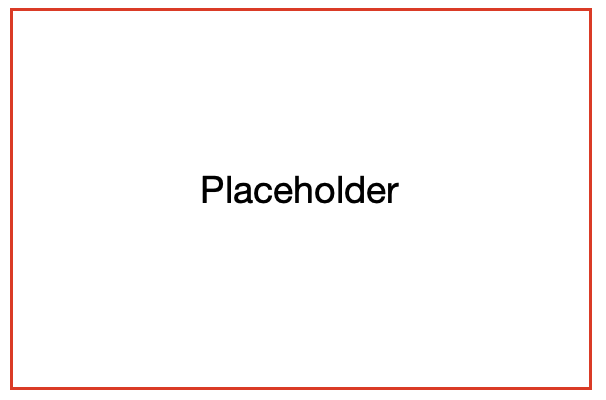
\includegraphics[width=0.5\linewidth]{texfiles/mech/eimg/cooling/placeholder}
  \caption{Coolant pump}
  \label{fig:Coolant Pump}
\end{figure}

\subsubsection{Coolant Storage Tank}
The cooling system is designed with consideration for the realistic scenario of the pod traveling through a low-pressure tube (near vacuum), limiting heat exchange with the atmosphere. The coolant in the circuit absorbs heat from the motor, battery, and traction controller, causing an increase in coolant temperature over time. The current design ensures sufficient coolant storage to keep all components well below the required maximum operating temperature.

For the hyperloop pod slated for participation in the European Hyperloop Week, a typical vehicle coolant tank with a capacity of 1 liter has been deemed adequate. This capacity aligns with the demands of the pod's cooling requirements, guaranteeing optimal performance throughout its operation.
\begin{figure}[ht]
  \centering
  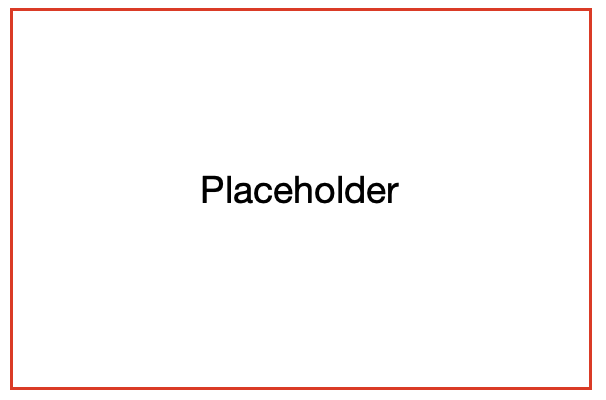
\includegraphics[width=0.5\linewidth]{texfiles/mech/eimg/cooling/placeholder}
  \caption{Coolant tank}
  \label{fig:Coolant tank}
\end{figure}

\subsubsection{Water Jackets}
The water jacket for the motor will be provided by the motor manufacturer, ensuring compatibility and optimal performance. For the water jackets of the traction controller and battery, custom fabrication will be undertaken based on the recommendations provided by their respective manufacturers. This approach guarantees that each component receives tailored cooling solutions to meet its specific requirements and operating conditions.

\subsubsection{Piping}
Two piping options are under consideration.
 i) CPVC pipes, chosen for their resistance to high temperatures, scaling, durability, low cost, and ease of installation. The specific piping route is yet to be finalized , but the total length is estimated to be around 6 meters. 
ii) The potential use of soft tubing is also being explored.

\subsection{Heat Exchanger}
\subsubsection{Role and Benefits in the cooling System}
In the context of the cooling system described for the hyperloop pod, a heat exchanger would play a crucial role in transferring heat between the coolant circulating within the closed-loop system and the surrounding environment. As the coolant circulates through the system, it absorbs heat from the motor, battery, and traction controller, thereby increasing in temperature. Since the hyperloop pod operates in a low-pressure tube with limited heat exchange with the atmosphere, the heat exchanger facilitates the dissipation of heat even in this constrained environment.

\begin{figure}[ht]
  \centering
  \subfloat[Closed View]{
    \centering
    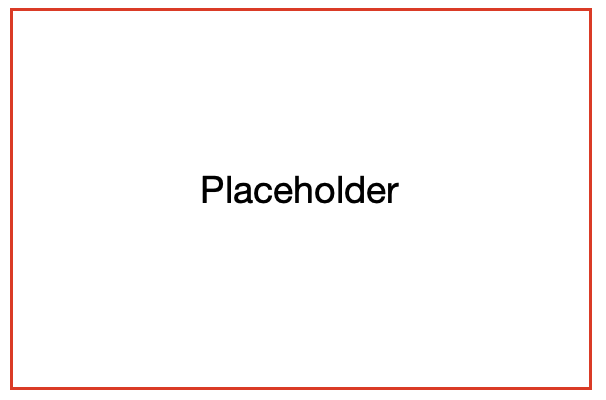
\includegraphics[width=0.5\linewidth]{texfiles/mech/eimg/cooling/placeholder}
    \label{fig:HE Closed view}
  }
  \subfloat[Open View]{
    \centering
    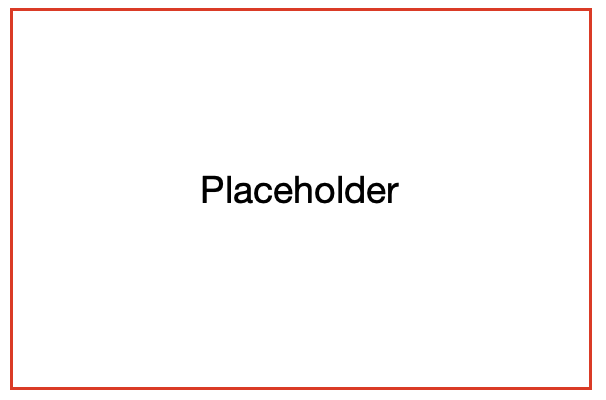
\includegraphics[width=0.5\linewidth]{texfiles/mech/eimg/cooling/placeholder}
    \label{fig:HE Open view}
  }
  \caption{Gyroid Heat Exchanger}
  \label{fig:HE}
\end{figure}


\subsubsection{Use of Phase Change Materials (PCMs)}
Introducing the heat exchanger utilizing phase change materials (PCMs) into the cooling system for the hyperloop pod would offer several advantages and could enhance its performance in specific scenarios, incorporating a heat exchanger with the use of phase changing material serves several important purposes:

\begin{itemize}
  \item \textbf{Enhanced Heat Absorption and Release:} The PCM, such as stearic acid, can absorb and release a significant amount of heat during its phase transition from solid to liquid and vice versa. Integrating a heat exchanger with PCM allows for efficient absorption of excess heat generated by components like the motor, traction controller, and battery.
  \item \textbf{Temperature Regulation:} By absorbing excess heat from critical components, the heat exchanger helps regulate their temperatures within the specified operating ranges. This prevents overheating, which can lead to performance degradation or damage to components.
  \item \textbf{Thermal Energy Storage:} The PCM's ability to store thermal energy during its phase change enables the system to store heat when temperatures are within acceptable limits and release it when needed to maintain optimal operating conditions. This helps in managing transient heat loads and stabilizing temperatures over time.
  \item \textbf{Reduced Coolant Temperature:} By utilizing the PCM's heat absorption capacity, the heat exchanger can lower the temperature of the coolant circulating in the system. This ensures that the coolant remains within acceptable temperature limits, contributing to the overall effectiveness of the cooling system.
  \item \textbf{Increased Efficiency:} Integrating a heat exchanger with PCM can improve the overall efficiency of the cooling system by maximizing heat transfer capabilities and reducing the reliance on conventional cooling methods alone.
  \item \textbf{Extended Operating Time:} The thermal energy stored in the PCM can be utilized to extend the operating time of the system before coolant temperature rises beyond acceptable levels. This can be particularly beneficial during transient operating conditions or in the event of temporary power interruptions.
\end{itemize}

Overall, incorporating a heat exchanger with the use of phase changing material adds an additional layer of heat management capability to your cooling system, contributing to improved performance, efficiency, and reliability in the hyperloop pod environment.


\subsubsection{Stearic Acid}

Stearic acid stands out as a highly versatile phase change material (PCM) deployed across diverse applications. Its unique characteristic of transitioning from solid to liquid state at a precise temperature renders it exceptionally suitable for thermal energy storage purposes. Through this phase transition, stearic acid exhibits remarkable heat absorption and release capabilities, making it a valuable asset in scenarios demanding efficient temperature regulation and thermal energy management. Commonly found in applications ranging from building insulation to specialized temperature control systems, stearic acid's efficacy as a PCM underscores its widespread industrial utility.

\paragraph{Stearic Acid}
Stearic acid is a saturated fatty acid with the chemical formula \( C_{18}H_{36}O_2 \). It is a long-chain carboxylic acid, meaning it has 18 carbon atoms in its hydrocarbon chain and a carboxyl group (COOH) at one end. Here are some key properties and uses of stearic acid:

\subparagraph{Physical Properties:}
\begin{itemize}
  \item Melting Point: Stearic acid is a solid at room temperature and has a melting point of around \( 69-70 \) degrees Celsius (\( 156-158 \) degrees Fahrenheit).
  \item Appearance: It is a white, waxy solid with a characteristic fatty odor.
\end{itemize}

\subparagraph{Chemical Properties:}
\begin{itemize}
  \item Structure: Stearic acid has a straight-chain structure with 18 carbon atoms, making it a saturated fatty acid. Hydrophobic: Like other fatty acids, stearic acid is hydrophobic, meaning it repels water.
\end{itemize}

In summary, stearic acid is a versatile compound with various industrial applications, and its phase change properties make it useful in thermal energy storage applications as well.

\subsection{Calculations and Simulations}

\textbf{WILL BE ADDED SOON (Dino)}
\subsection{Safety Measures}
Given the close integration of the cooling system with the electronic systems, the primary risk is a coolant leak that could potentially damage electronic components. Preventive measures are outlined in the table below, and deionised water is chosen as the preferred coolant due to its low conductivity.
\subsubsection{Potential Failure Modes and Risk Mitigation-}
\begin{itemize}
  \item \textbf{Coolant Leaks}
    \begin{itemize}
      \item Effect of Failure: Damage Electronic components
      \item Root Cause: Poor sealing at pipe joints
      \item Risk Mitigation Strategy: Maintain the correct coolant level, avoid overfilling the tank, sealing pipes with hose clamps and use deionized water as a coolant.
    \end{itemize}
  \item \textbf{Temperature of Critical component rises above rated temperature}
    \begin{itemize}
      \item Effect of Failure: Damage Component
      \item Root Cause: Insufficient cooling due to prolonged operation
      \item Risk Mitigation Strategy: Implement a control system to halt the motor and by installing two temperature sensors if temperatures exceed prescribed limits for the motor, battery, or traction controller.
    \end{itemize}
  \item \textbf{Temperature of Critical component rises above rated temperature}
    \begin{itemize}
      \item Effect of Failure: Coolant Leaks
      \item Root Cause: Insufficient cooling due to air traps or exceeding defined operation time
      \item Risk Mitigation Strategy: Position of the system including heat exchanger is placed at the front of the pod, in order to purge air after refilling, and adhere to defined operation times.
    \end{itemize}
  \item \textbf{Blocks in piping}
    \begin{itemize}
      \item Effect of Failure: Insufficient cooling and damage to components
      \item Root Cause: Foreign particles/debris
      \item Risk Mitigation Strategy: Introduce filters in the piping system and conduct regular cleaning maintenance.
    \end{itemize}
\end{itemize}


\subsubsection{FMEA analysis}

\textbf{Failure Mode: Coolant Leaks}
\begin{itemize}
  \item Effects of Failure: Damage to Electronic components
  \item Severity: High
  \item Causes of Failure: Poor sealing at pipe joints
  \item Occurrence: Medium
  \item Current Controls: Regular inspection for leaks, pressure testing of the system
  \item Detection: Visual inspection, pressure sensors
  \item Risk Priority Number (RPN): Severity * Occurrence * Detection
  \item Recommended Actions: Improve seal quality, implement redundant sealing, increase inspection frequency
  \item Responsibility: Mechanical Team
  \item Actions Taken: Upgraded sealing materials, added secondary containment
  \item Revised RPN: After action taken
\end{itemize}

\textbf{Failure Mode: Temperature of Critical Component Rises Above Rated Temperature (First Instance)}
\begin{itemize}
  \item Effects of Failure: Damage to Component
  \item Severity: High
  \item Causes of Failure: Insufficient cooling due to prolonged operation
  \item Occurrence: High
  \item Current Controls: Thermal cutoff switches, temperature monitoring
  \item Detection: Thermal sensors with automated system feedback
  \item Risk Priority Number (RPN): Severity * Occurrence * Detection
  \item Recommended Actions: Implement more efficient cooling mechanisms, revise operational protocols to prevent prolonged operation without cooling
  \item Responsibility: Electrical Team
  \item Actions Taken: Included additional cooling systems, adjusted operational limits
  \item Revised RPN: After action taken
\end{itemize}

\textbf{Failure Mode: Temperature of Critical Component Rises Above Rated Temperature (Second Instance)}
\begin{itemize}
  \item Effects of Failure: Coolant Leaks
  \item Severity: High
  \item Causes of Failure: Insufficient cooling due to air traps or exceeding defined operation time
  \item Occurrence: Medium
  \item Current Controls: Coolant system design to avoid air traps, operational time limits
  \item Detection: Temperature and flow sensors
  \item Risk Priority Number (RPN): Severity * Occurrence * Detection
  \item Recommended Actions: Redesign of the coolant flow paths to eliminate air traps, strict adherence to operational time limits
  \item Responsibility: Design Team
  \item Actions Taken: Coolant flow paths optimized, operational procedures updated
  \item Revised RPN: After action taken
\end{itemize}

\textbf{Failure Mode: Blocks in Piping}
\begin{itemize}
  \item Effects of Failure: Insufficient cooling and damage to components
  \item Severity: Medium
  \item Causes of Failure: Foreign particles/debris
  \item Occurrence: Low
  \item Current Controls: Filtration systems, preventive maintenance schedules
  \item Detection: Flow rate monitoring, pressure differential sensors
  \item Risk Priority Number (RPN): Severity * Occurrence * Detection
  \item Recommended Actions: Improve filtration system, implement more rigorous maintenance and cleaning schedules
  \item Responsibility: Maintenance Team
  \item Actions Taken: Upgraded filters, more frequent cleaning
  \item Revised RPN: After action taken
\end{itemize}
\subsubsection{References}

\begin{figure}[ht]
  \centering
  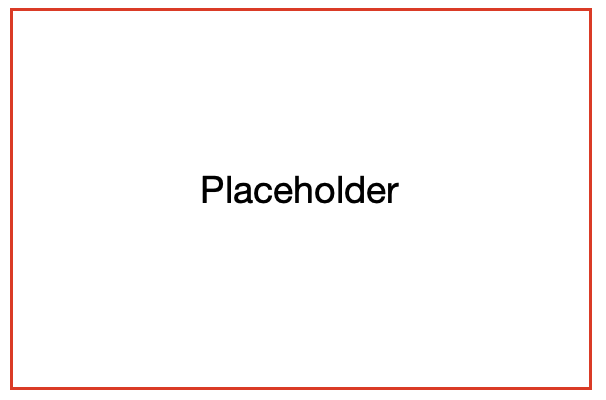
\includegraphics[width=\linewidth]{texfiles/mech/eimg/cooling/placeholder}
  \caption{Flowchart of the system}
  \label{fig:schematic}
\end{figure}

%add schematic








\newpage


% Traction Systems
\chapter{Traction System}

\section{Introduction}

\section{Propulsion}

\subsection{Overview}

To accelerate our Hyperloopod we use our EMRAX 188 electric motor from last season. This delivers an output of 60 kW under high voltage and a maximum torque of 100 Nm. This torque gets transferred to a right-angle gearbox and from there is slid to the drive wheels via cardan joints.

\subsubsection{Concept}
The main goal of this system is to accelerate our pod with an acceleration of \(5 \, \text{m/s}^2\). Since the given \(100 \, \text{Nm}\) are not sufficient under an estimated total weight of \(250 \, \text{kg}\), the drivetrain requires a gear ratio. Since an angular gearbox is installed anyway, it is easy to implement this criterion there. In order to maintain a relatively high top speed of the pod, this transmission ratio should be as close as possible. According to the formula
\[
T_{\text{required}} = \frac{{(m \cdot a + \frac{1}{2} \cdot \rho_{\text{air}} \cdot C_w \cdot A_{\text{Aeroshell}} \cdot v^2 + m \cdot g \cdot \cos(\Theta)) \cdot r}}{{\eta}}
\]
we know that we require at least around \(170 \, \text{Nm}\) of torque to achieve this amount of acceleration. While the pod weight of \(250 \, \text{kg}\) is only an estimate at the time of system design and we are always keen to get such complex parts from our partners, we opted for a \(2:1\) ratio of a Mädler gearbox. With this gear ratio, a respectable top speed of \(113 \, \text{km/h}\) is still possible. This is absolutely sufficient for our prototype, as we are still sticking to our basic idea: For low speeds and accelerations, we drive our hyperloop pod with a conventional wheel drive and for everything above that, the pod will hover with a linear induction motor which will be added in future prototypes. We believe that we can achieve an increase in efficiency in this way as permanent levitation is not necessary.

The transmitted torque must now be directed to the drive wheels in such a way that it is still possible to ensure a working suspension. For this, we use universal joints on both sides of the centered bevel gear. These also come from our partner Mädler and are connected to the bevel gear using in-house produced adapter shafts and feather keys. To finally connect the other ends of the shaft joints to the wheel, only one last shaft is missing. This is also fitted with a keyway on the joint side and a bolt circle on a flange on the wheel side. Now that the wheels are supplied with power, it is important to create sufficient rolling friction. To achieve this, Continental provides us with a rubber coating for our wheels. \\
Of course, this all has to be mounted into the chassis. For this, we use three different types of brackets beside the knuckles, where the wheelshafts are mounted: one for the motor, one for the motorshaft and two of the same kind, which carry everything between the shaft joints.

\subsubsection{Size, Components, and Appearance}

\autoref{table:components}
\begin{table}[ht]
\centering
\begin{adjustbox}{width=\textwidth}
\begin{tabular}{|>{\bfseries}m{2.5cm}|m{1.4cm}|m{1.7cm}|m{2.9cm}|m{2.2cm}|}
\hline
Component & Number & Mass [kg] & Size [mm] &  In-house/ outsourced \\
\hline
Motor & x1 & 7 & \(188 \times 188 \times 112\) &   Bought \\
Motorshaft & x1 & 0.4 & \(170 \times 83\times 83\) &Outsourced \\
Resolver & 1 & 1 & TS2620N21E11 &  Bought \\-.-.
Bevelgear z=20 & x1 & 3 & \(10 \times 90\) &  Bought \\
Bevelgear z=40 & x1 & 9.6 & \(20 \times 30 \times 50\) &Bought \\
Gearshaft Pressfitted & x1 & 0.3 & \(103 \times 40 \times 40\) & Outsourced \\
Gearshaft bolted & x1 & 0.7 & \(106 \times 55 \times 55\) &Outsourced \\
Shaft Joint & x2 & 4.1 & \(30 \times 40 \times 60\) &  Bought \\
Wheelshaft & x2 & 0.7 & \(138 \times 100 \times 100\) &   Outsourced \\
Wheel & x2 & 1.7 & \(200 \times 200 \times 155\) &  Outsourced \\
\hline
\end{tabular}
\end{adjustbox}
\caption{Components}
\label{table:components}
\end{table}

\subsection{Design Process and Appearance}

\subsubsection{Motor}

\begin{figure}[H]
\centering
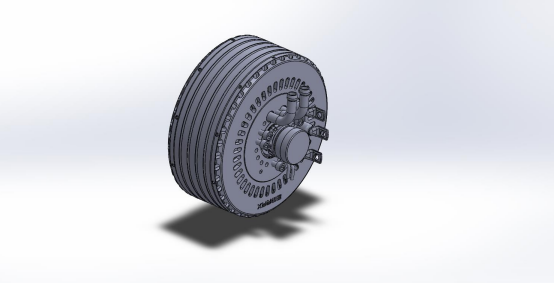
\includegraphics[width=0.6\textwidth]{texfiles/mech/eimg/propulsion/picture_motor}
\caption{CAD of EMRAX 188}
\label{}
\end{figure}

As previously mentioned, we are once again using our EMARX 188 electric motor from last season. You can find all the technical details in Table~\ref{tab: Motor Specifications} .



\subsubsection{Motorshaft}

\begin{figure}[ht!]
  \centering
  \begin{subfigure}{.5\textwidth}
    \centering
    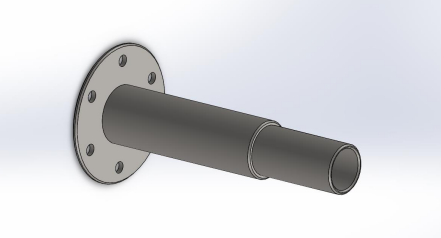
\includegraphics[width=\linewidth]{texfiles/mech/eimg/propulsion/picture_motorshaft}
    \caption{CAD Render}
    \label{fig:CAD Motorshaft}
  \end{subfigure}%
  \begin{subfigure}{.4\textwidth}
    \centering
    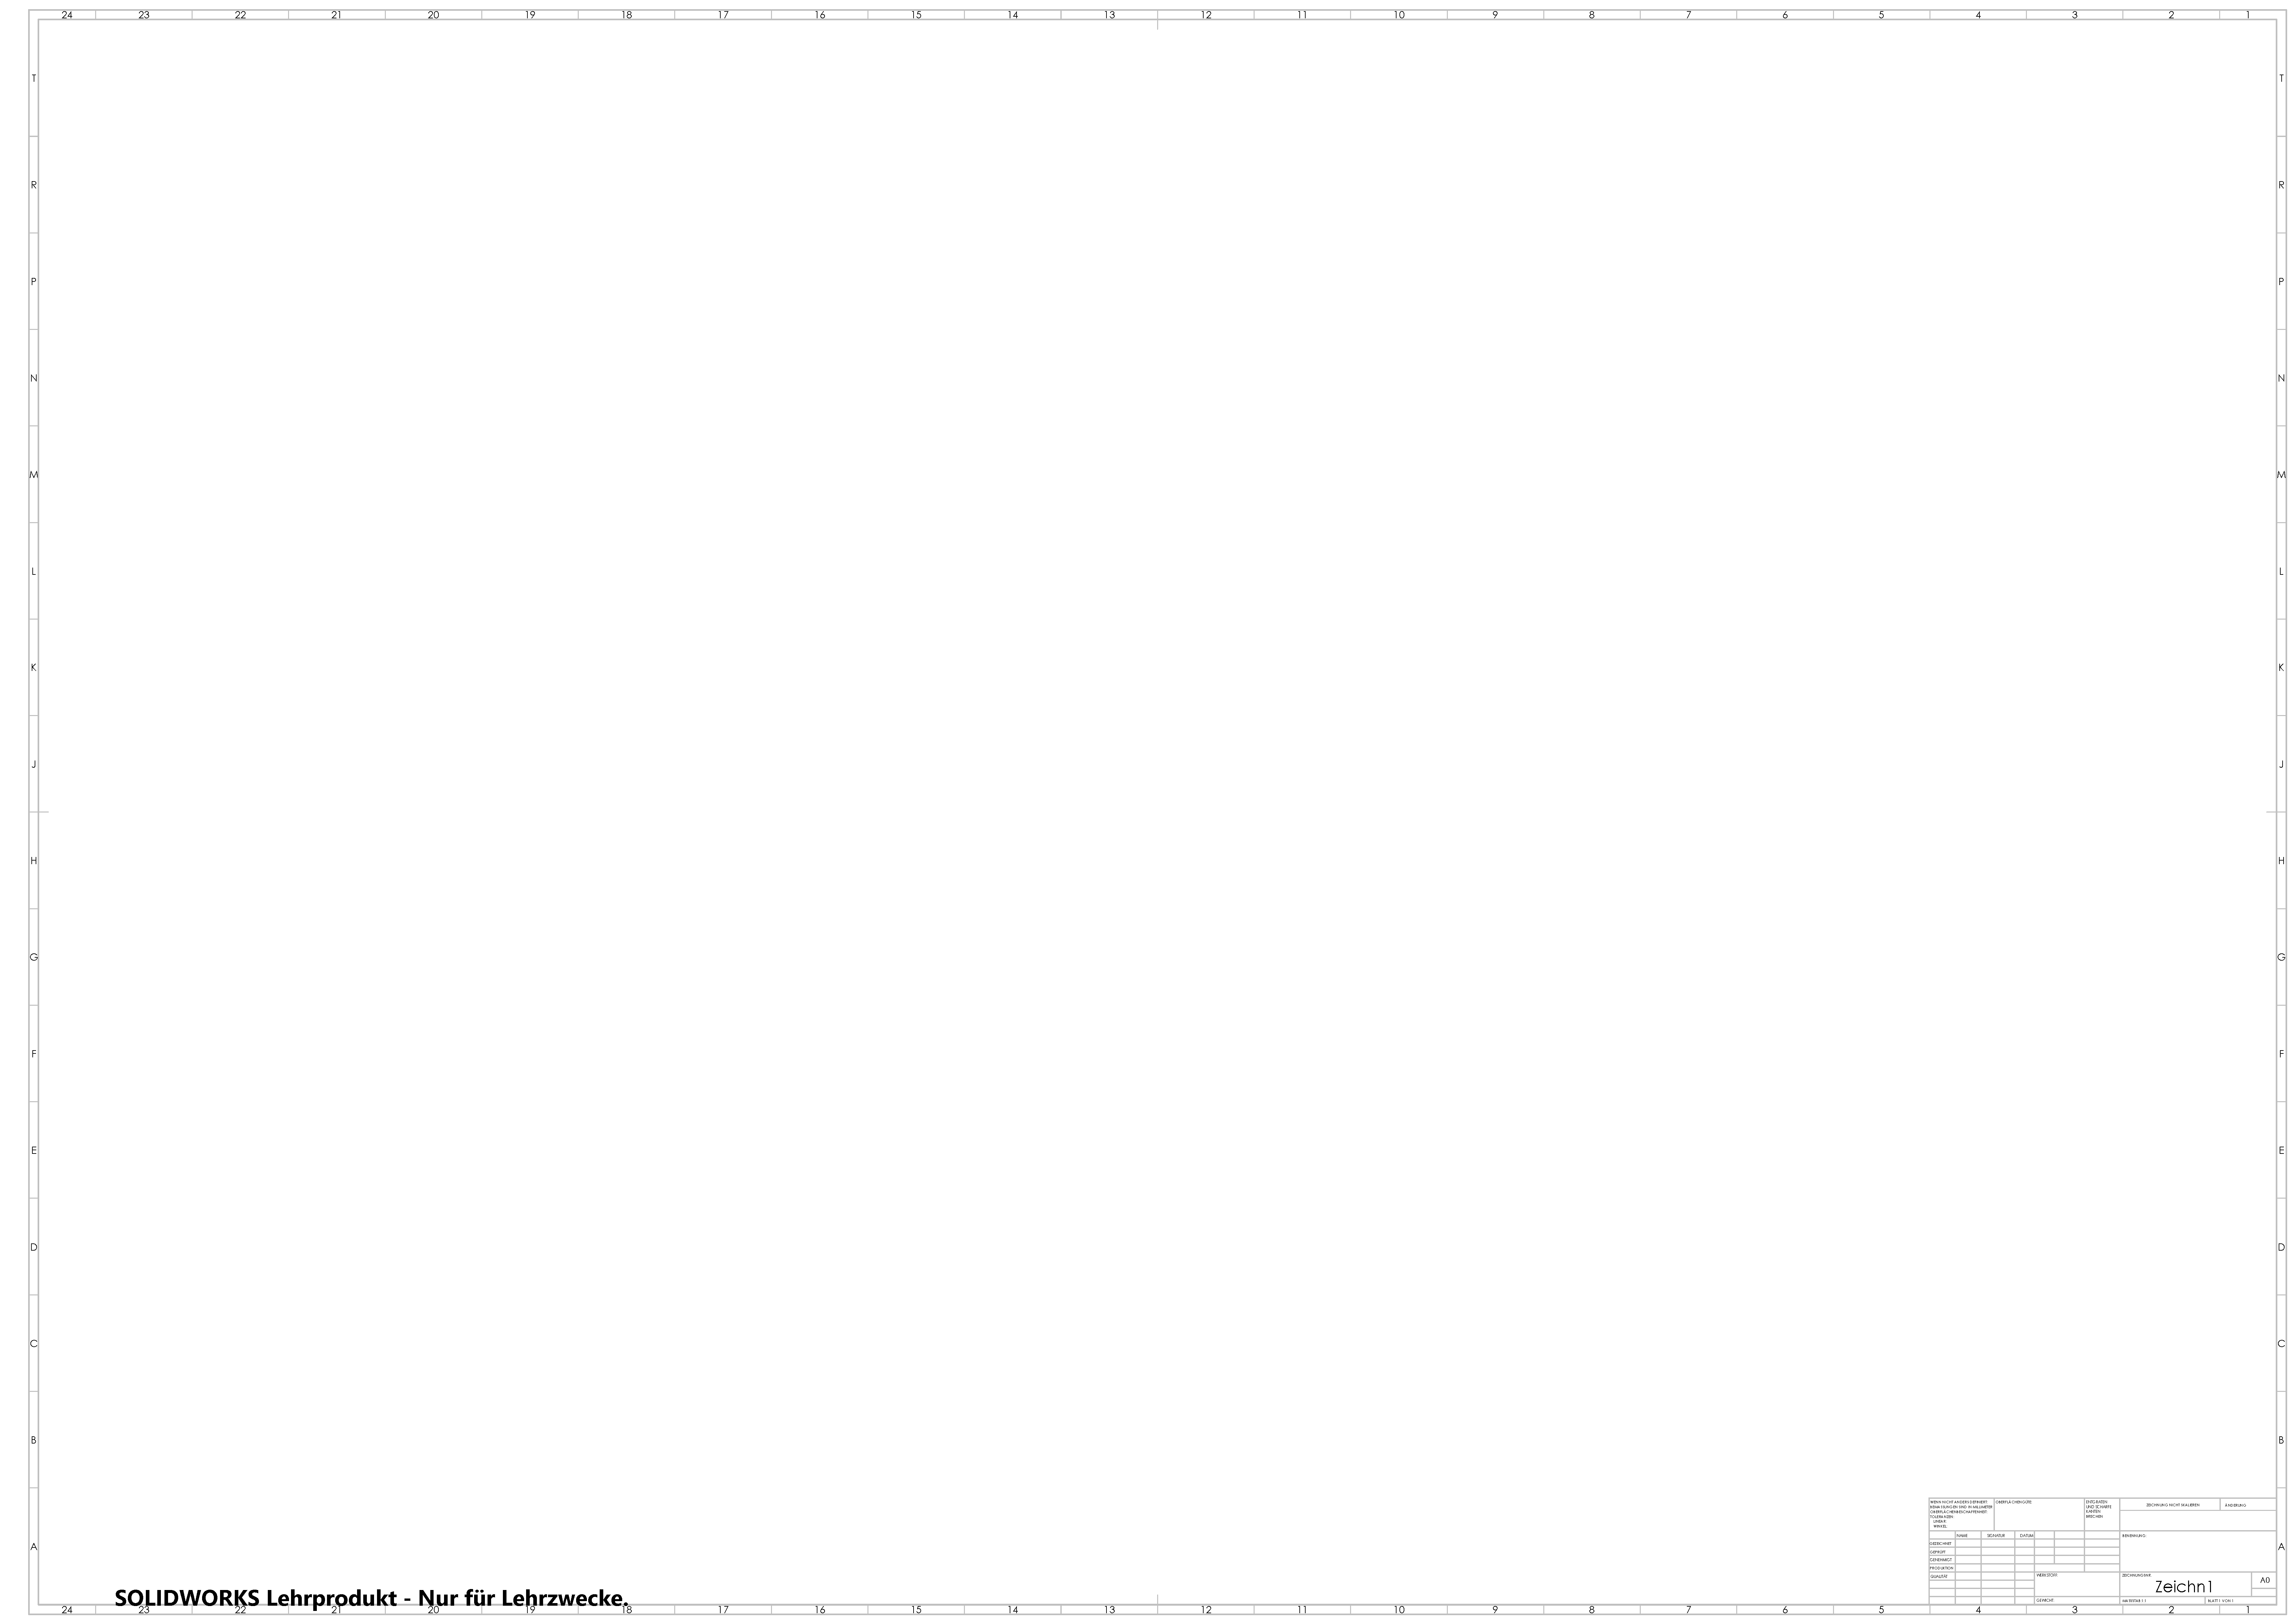
\includegraphics[width=\linewidth]{texfiles/mech/eimg/propulsion/spaceholder_technical_drawing}
    \caption{Technical Drawing}
    \label{fig:TD Motorshaft}
  \end{subfigure}
  \caption{Motor Bracket}
  \label{fig:Motorshaft}
\end{figure}



Even though it is a heavy material, C45 steel provides adequate tensile strength to transmit torque from the motor to the gearbox or from the gearbox to the wheels. To maintain a relatively low weight for this part, it is hollow like all the other shafts. In Figure \ref{fig:motorshaft_forces}, you can now see the applied forces. The shaft is mounted on the motor at the screw holes of the flange (green). This means that the motor torque of \(100 \, \text{Nm}\) (pink) acts up to the surface on which the bevel gear is pressed. The calculation of the contact pressure of \(16.26 \, \text{MPa}\) is given by
\[
p_{\text{contact}}=\frac{2\cdot M\cdot S_r}{\pi \cdot D^2 \cdot l\cdot \mu}
\]
In addition, there is a centrifugal force (blue) at maximum rotational speed of \(6000 \, \text{rpm}\).

\autoref{fig:motorshaft_forces}
\begin{figure}[H]
\centering
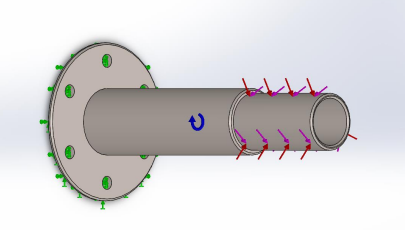
\includegraphics[width=0.6\textwidth]{texfiles/mech/eimg/propulsion/picture_forces_motorshaft}
\caption{Forces acting on the Motorshaft}
\label{fig:motorshaft_forces}
\end{figure}

\subsubsection{Bevel Gears}
picture gearbox

The bevel gears with the article numbers 36736000 and 36736100 are our choice to fulfill the desired purpose.
36736000 offers spur gearing with 20 teeth. With a maximum permissible torque of 130 Nm, it can withstand the prevailing forces. 
The larger counterpart 36736100 therefore has twice as many teeth (40 teeth) and is designed for a maximum torque of 260 Nm.

\subsubsection{Gearshafts}
\begin{figure}[H]
\centering
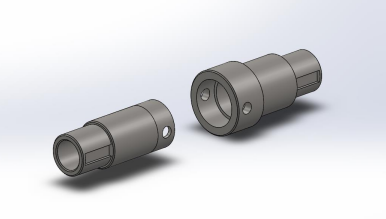
\includegraphics[width=0.6\textwidth]{texfiles/mech/eimg/propulsion/picture_gearshafts}
\caption{}
\label{}
\end{figure}

To be able to conduct the torque of the bevel gear, we have designed another shaft. This consists of two individual parts, one which is again pressed into the bevel gear and the other which is screwed onto the first part after pressing.
The specifications of the initially acting shaft are as follows:

\begin{figure}[ht!]
  \centering
  \begin{subfigure}{.5\textwidth}
    \centering
    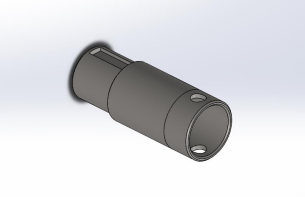
\includegraphics[width=\linewidth]{texfiles/mech/eimg/propulsion/picture_gearshaft_right}
    \caption{CAD Render}
    \label{fig:CAD Motorshaft}
  \end{subfigure}%
  \begin{subfigure}{.5\textwidth}
    \centering
    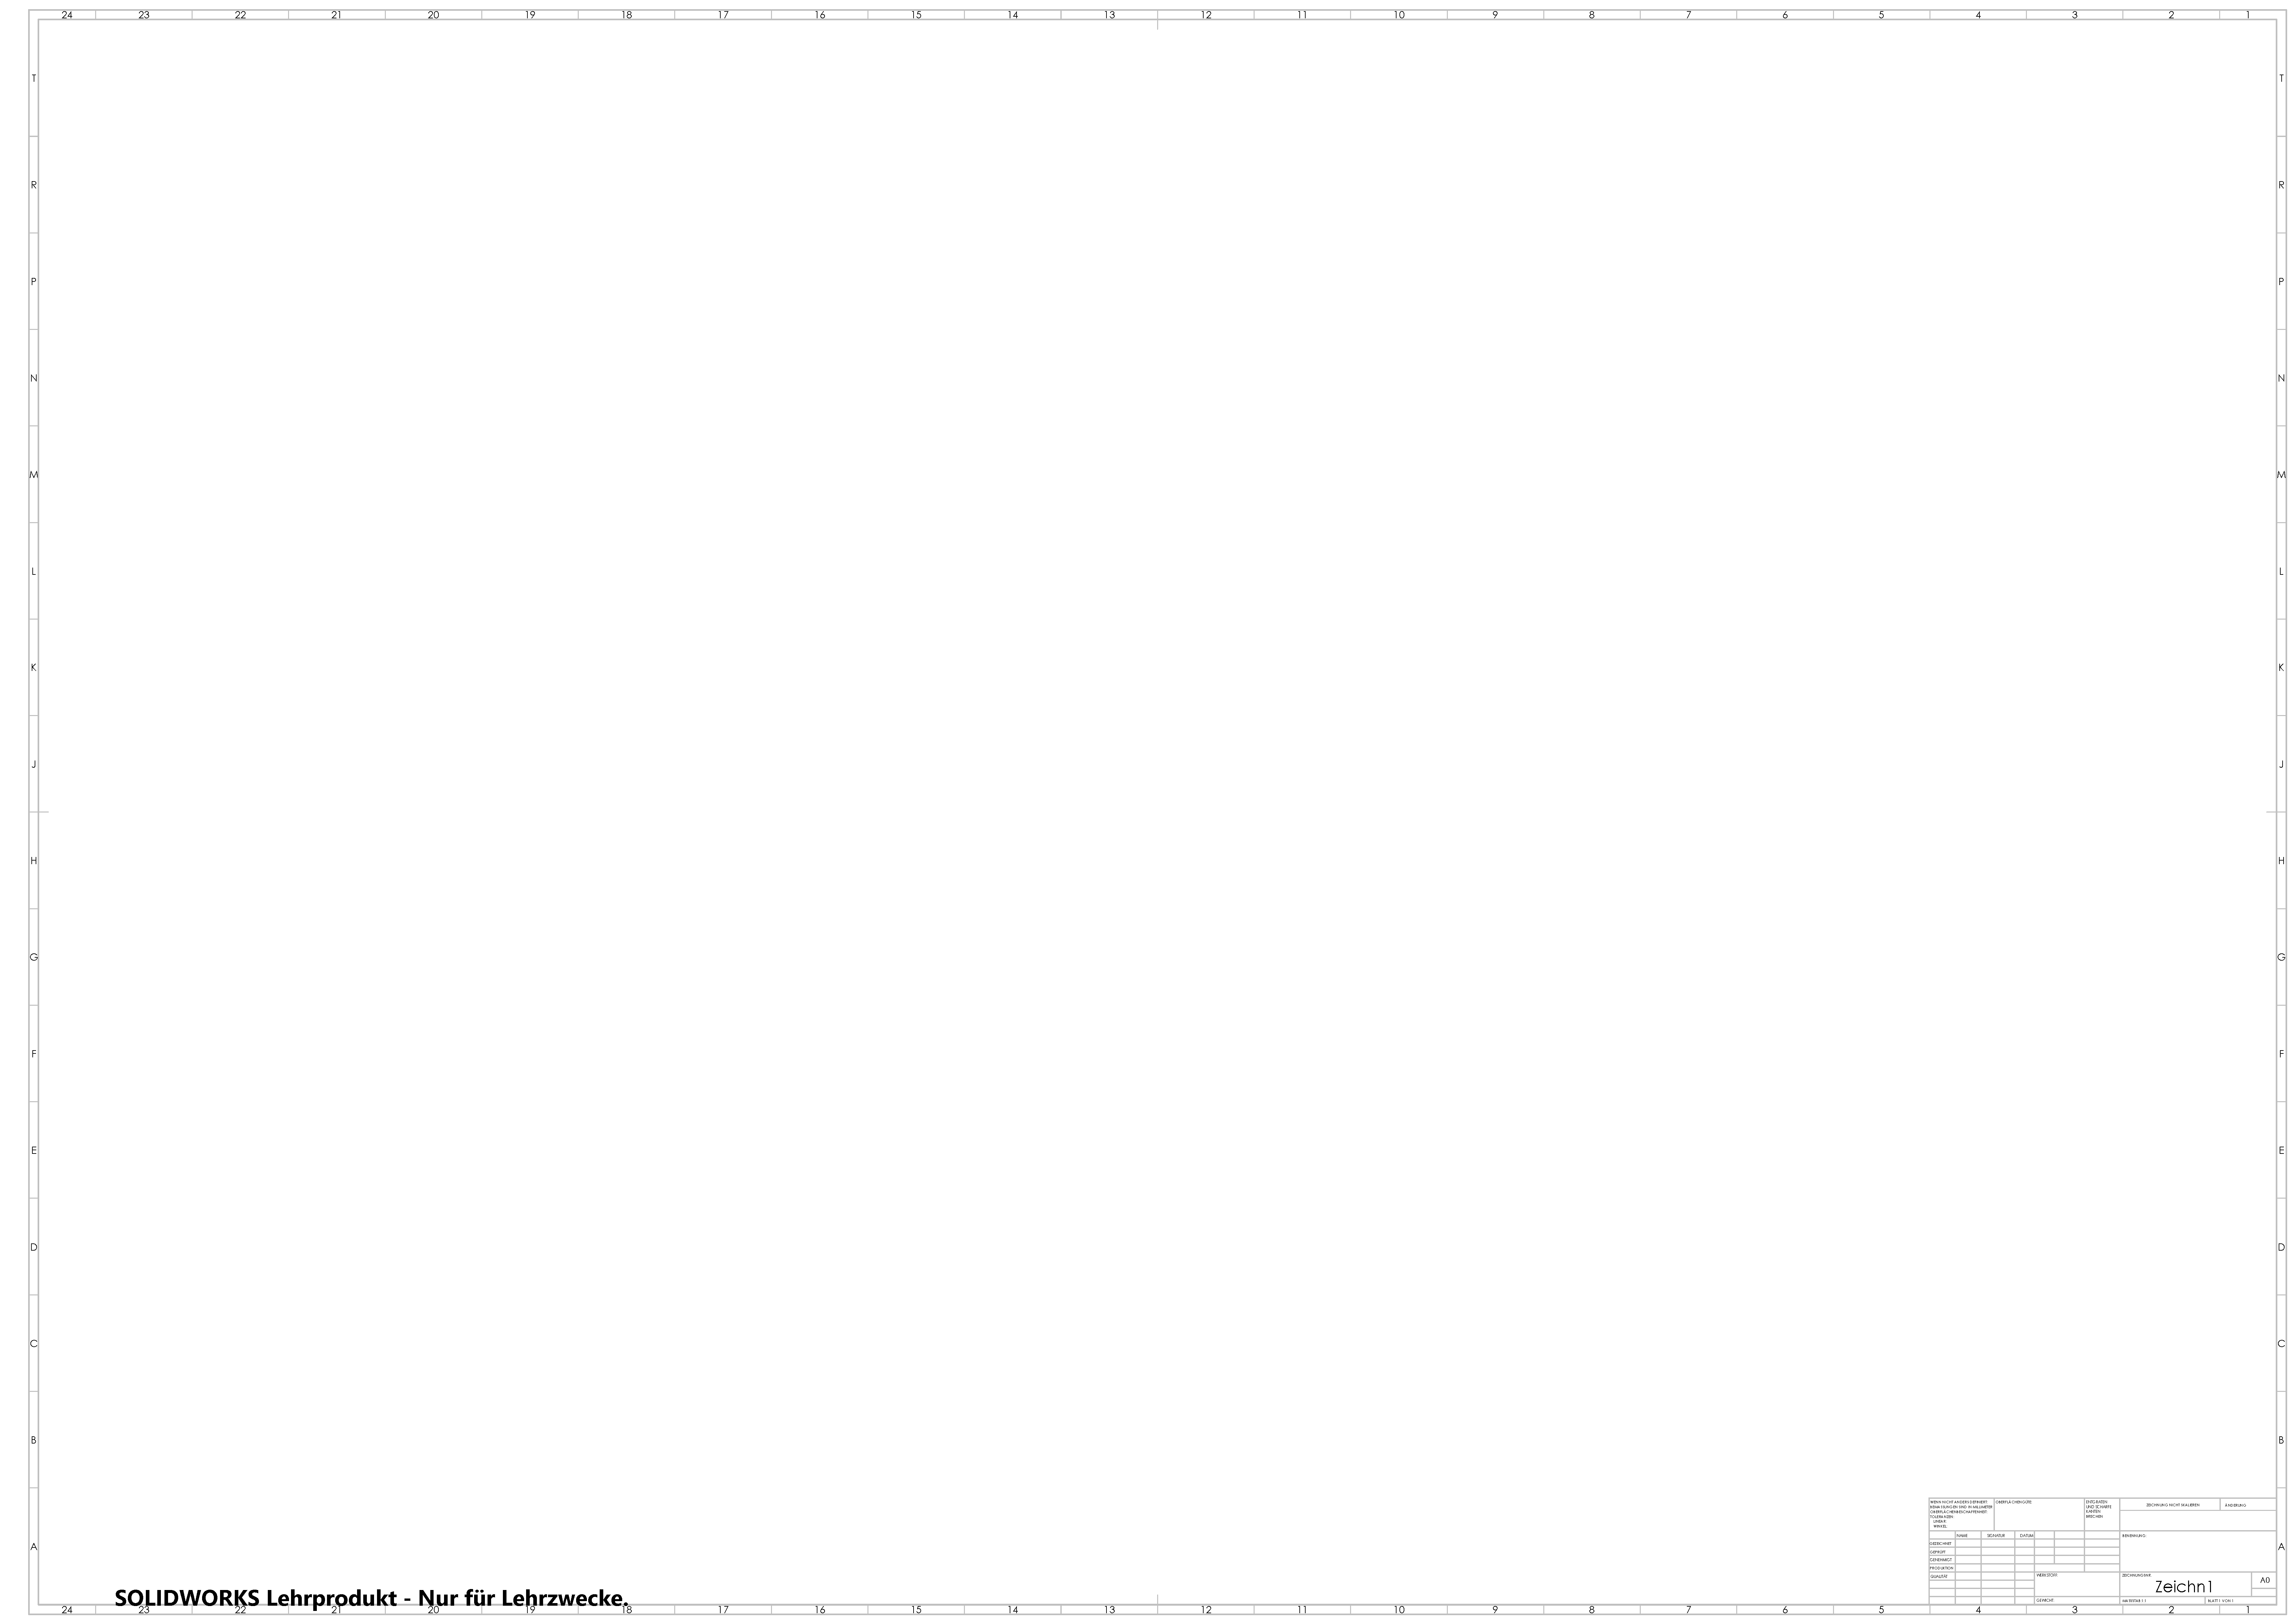
\includegraphics[width=\linewidth]{texfiles/mech/eimg/propulsion/spaceholder_technical_drawing}
    \caption{Technical Drawing}
    \label{fig:TD Motorshaft}
  \end{subfigure}
  \caption{Motor Bracket}
  \label{fig:Motorshaft}
  \end{figure}



Fig.xx  shows all the acting forces. For calculating the pressing force (red) we again use the formula for \(p_{\text{contact}}\)
and get the result of \(21.22 \, \text{MPa}\). The higher torque of \(200 \, \text{Nm}\) (pink) resulting from the gear ratio also acts on this surface and is transferred to the screw holes and keyway (green). A centrifugal force (blue) also acts on this part, but this has now been halved by the gear ratio and is therefore only based on \(3000 \, \text{rpm}\). Finally, we assume a bearing restraint (orange) at the shaft end to the shaft joint. The admissibility of this case is described in the paragraph on the shaft joint itself.

\begin{figure}[H]
\centering
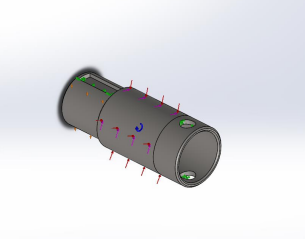
\includegraphics[width=0.6\textwidth]{texfiles/mech/eimg/propulsion/picture_forces_gearshaft_right}
\caption{Forces acting on the pressfitted Gearshaft}
\label{fig:gearshaft_right_forces}
\end{figure}


The torque is now transferred to the second part of the gearshaft:
\begin{figure}[ht!]
  \centering
  \begin{subfigure}{.5\textwidth}
    \centering
    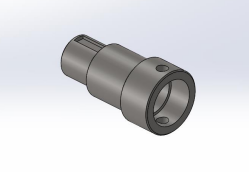
\includegraphics[width=\linewidth]{texfiles/mech/eimg/propulsion/picture_gearshaft_left}
    \caption{CAD Render}
    \label{fig:CAD Motorshaft}
  \end{subfigure}%
  \begin{subfigure}{.5\textwidth}
    \centering
    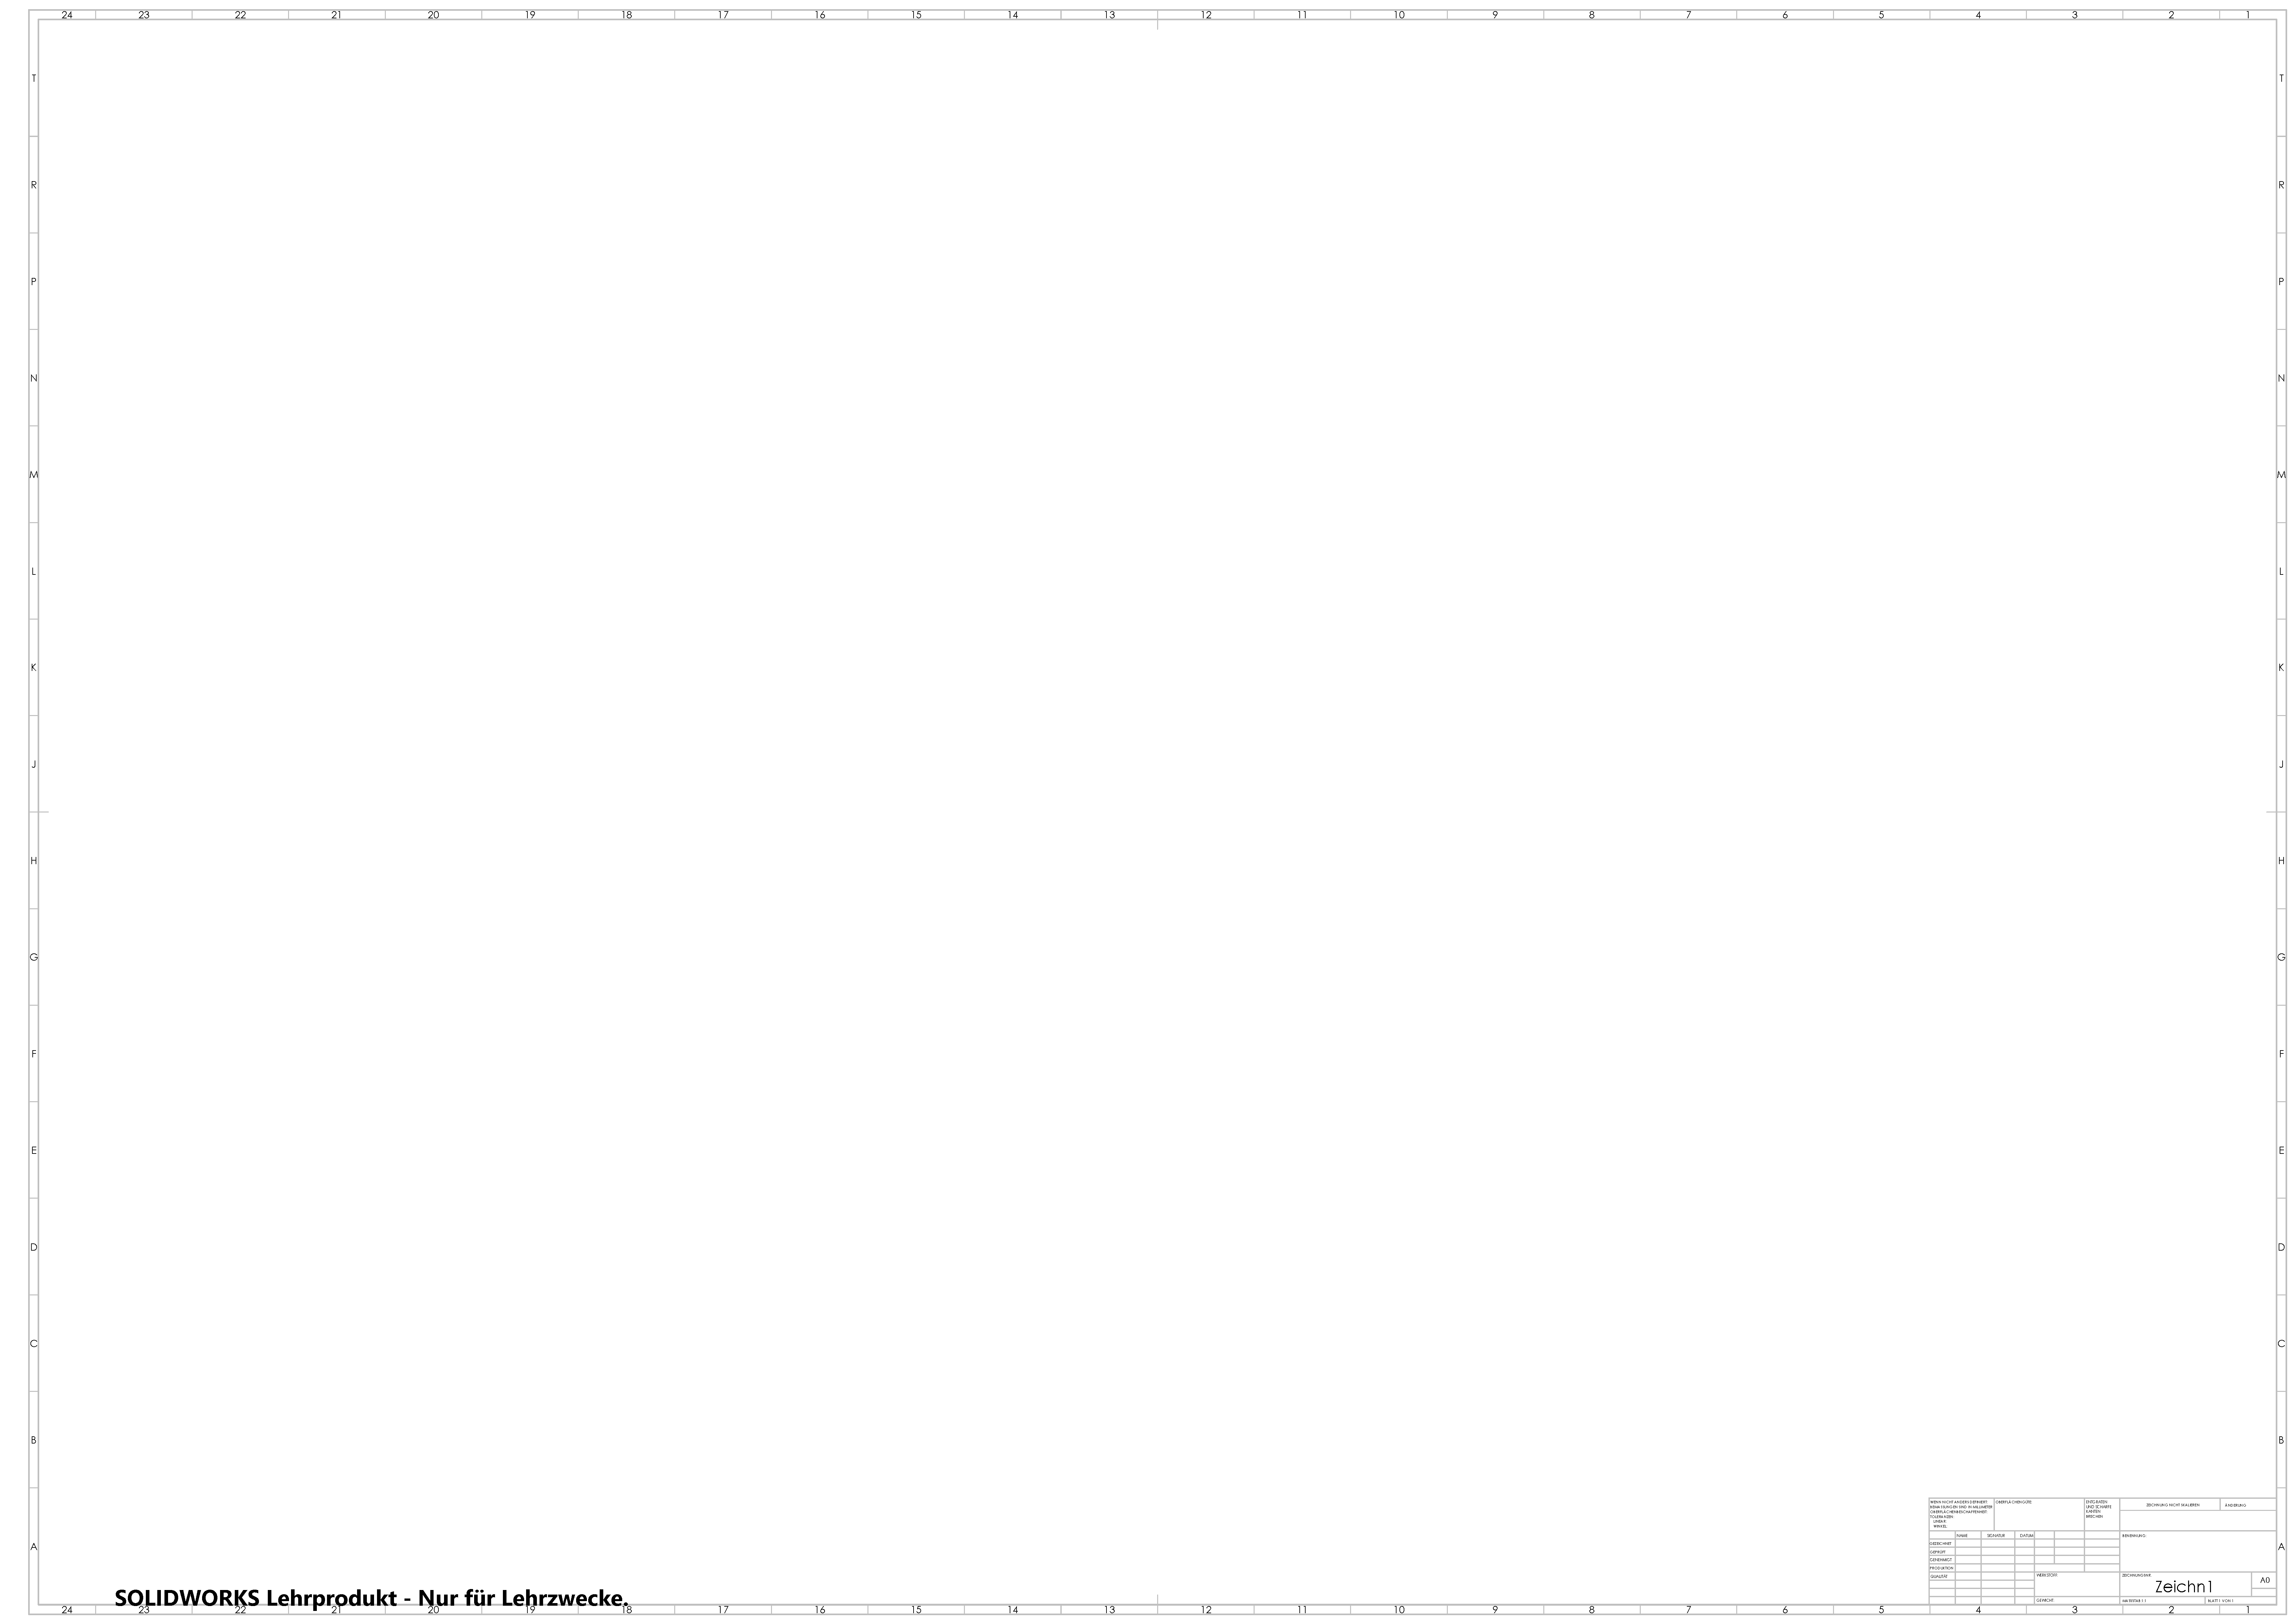
\includegraphics[width=\linewidth]{texfiles/mech/eimg/propulsion/spaceholder_technical_drawing}
    \caption{Technical Drawing}
    \label{fig:TD Motorshaft}
  \end{subfigure}
  \caption{Motor Bracket}
  \label{fig:Motorshaft}
  \end{figure}



Fig.xx shows all the forces acting on this part. The two shafts are connected to each other at the screw holes (green). The centrifugal force (blue) acts as in the first shaft at \(3000 \, \text{rpm}\) and the torque of \(200 \, \text{Nm}\) (pink) up to the keyway. This end piece of the shaft is also simulated as a bearing (orange).

\begin{figure}[H]
\centering
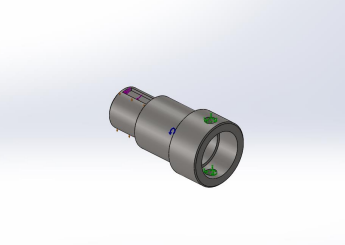
\includegraphics[width=0.6\textwidth]{texfiles/mech/eimg/propulsion/picture_forces_gearshaft_left}
\caption{Forces acting on the bolted Gearshaft}
\label{fig:gearshaft_left_forces}
\end{figure}

\subsubsection{Shaft Joints}
\begin{figure}[H]
\centering
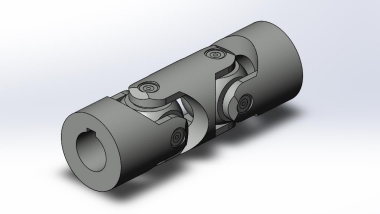
\includegraphics[width=0.6\textwidth]{texfiles/mech/eimg/propulsion/picture_shaft_joint}
\caption{}
\label{}
\end{figure}


To enable the system to absorb shocks, we use cardan shafts on each side. This allows the wheels to move vertically independently of the rest of the pod. Our partner Mädler is once again supplying us with such complex parts. Item number 63167000N is a double universal joint which we install in our system. It has a keyway at both ends and is designed to transmit 202 Nm at 3000 rpm. These specifications are almost perfect for our drive power.
We will mount the heart of our system at the ends of this joint adjacent to the gearbox. This is also the reason why a bearing is created at the respective ends in the simulations of the shafts because this bearing is also attached above the respective area.
However, more on the bearing and attachment points will follow in the corresponding sections.

\subsubsection{Wheelshafts}
\begin{figure}[ht!]
  \centering
  \begin{subfigure}{.5\textwidth}
    \centering
    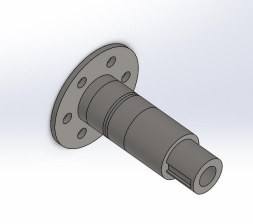
\includegraphics[width=\linewidth]{texfiles/mech/eimg/propulsion/picture_wheelshaft}
    \caption{CAD Render}
    \label{fig:CAD Motorshaft}
  \end{subfigure}%
  \begin{subfigure}{.5\textwidth}
    \centering
    \includegraphics[width=\linewidth]{texfiles/mech/eimg/propulsion/spaceholder_technical_drawing}
    \caption{Technical Drawing}
    \label{fig:TD Motorshaft}
  \end{subfigure}
  \caption{Motor Bracket}
  \label{fig:Motorshaft}
  \end{figure}


The wheel shafts provide the mounting point for the wheels. This is done by means of a bolt circle on a flange to ensure easy mounting and, if necessary, changing of the wheels. In this shaft, the 200 Nm torque (pink) applied to the keyway is transmitted to the wheel over the entire surface of the flange. The centrifugal force (blue) is also generated again due to the 3000 rpm and this shaft is also mounted on bearings (orange) within the knuckles. You can find out more about this bearing in the suspension section. However, this shaft must be able to withstand the mass inertia of the wheel (red). This is calculated by
\(5/2 \times m_{\text{wheel}} \times a\)

\begin{figure}[ht]
\centering
\includegraphics[width=0.6\textwidth]{texfiles/mech/eimg/propulsion/picture_forces_wheelshaft}
\caption{Forces acting on the wheelshaft}
\label{fig:wheelshaft_forces}
\end{figure}

\subsubsection{Wheels}
\begin{figure}[ht!]
  \centering
  \begin{subfigure}{.5\textwidth}
    \centering
    \includegraphics[width=\linewidth]{texfiles/mech/eimg/propulsion/picture_wheel}
    \caption{CAD Render}
    \label{fig:CAD Motorshaft}
  \end{subfigure}%
  \begin{subfigure}{.5\textwidth}
    \centering
    \includegraphics[width=\linewidth]{texfiles/mech/eimg/propulsion/spaceholder_technical_drawing}
    \caption{Technical Drawing}
    \label{fig:TD Motorshaft}
  \end{subfigure}
  \caption{Motor Bracket}
  \label{fig:Motorshaft}
 
\end{figure}

Finally, we transfer the torque (pink) to the wheels via the contact surface of the flange (green). The mass inertia of the wheel (red)
\(5/2 \times m_{\text{wheel}} \times a\)
, again the centrifugal force at 3000 rpm (blue) and the local pod weight of approximately 600 N (orange) also have an effect here. This weight, together with the rolling friction coefficient of the rubber cover, enables slip-free propulsion. We get this coefficient of 0,5099 by the formula
\[
\frac{m \cdot a}{m \cdot g}
\]

\begin{figure}[H]
\centering
\includegraphics[width=0.6\textwidth]{texfiles/mech/eimg/propulsion/picture_forces_wheel}
\caption{Forces acting on the wheels}
\label{fig:wheel_forces}
\end{figure}


\subsubsection{Motorbracket}

\begin{figure}[ht!]
  \centering
  \begin{subfigure}{.5\textwidth}
    \centering
    \includegraphics[width=\linewidth]{texfiles/mech/eimg/propulsion/placeholder}
    \caption{CAD Render}
    \label{fig:CAD Motorbracket}
  \end{subfigure}%
  \begin{subfigure}{.5\textwidth}
    \centering
    \includegraphics[width=\linewidth]{texfiles/mech/eimg/propulsion/placeholder}
    \caption{Technical Drawing}
    \label{fig:TD Motorbracket}
  \end{subfigure}
  \caption{Motor Bracket}
  \label{fig:Motorbracket}
\end{figure}

Our motor is mounted in the chassis using a bracket. This contains all the holes for screws and other components that protrude to the rear. End plates with screw holes are welded to four arms to finally screw () them into the chassis. The torque () and the inertia of the motor () prevail at this bracket.

\begin{figure}[H]
\centering
\includegraphics[width=0.6\textwidth]{texfiles/mech/eimg/propulsion/placeholder}
\caption{Forces acting on the motorbracket}
\label{fig:motorbracket_forces}
\end{figure}

\subsubsection{Motorshaftbracket}
\begin{figure}[H]
\centering
\includegraphics[width=0.6\textwidth]{texfiles/mech/eimg/propulsion/placeholder}
\caption{}
\label{}
\end{figure}

\begin{figure}[H]
\centering
\includegraphics[width=0.6\textwidth]{texfiles/mech/eimg/propulsion/placeholder}
\caption{}
\label{}
\end{figure}

To finally support this first area of the drive system, we also support the shaft that protrudes from the motor. This is done using the CHDF35 flangebearing from Misumi. This bearing is finally integrated into the chassis by another bracket. Only the weight of the motor shaft (), its mass inertia and the wheight of the flangebearing () act on this bracket.

%\begin{figure}[H]
%\centering
%\includegraphics[width=0.6\textwidth]{texfiles/mech/eimg/propulsion/picture_forces_motorshaftbracket}
%\caption{Forces acting on the motorshaftbracket}
%\label{fig:motorshaftbracket_forces}
%\end{figure}

\subsubsection{Bearinghouse}
%\begin{figure}[H]
%\centering
%\includegraphics[width=0.6\textwidth]{texfiles/mech/eimg/propulsion/picture_bearinghouse}
%\caption{}
%\label{}
%\end{figure}

%\begin{figure}[H]
%\centering
%\includegraphics[width=0.6\textwidth]{texfiles/mech/eimg/propulsion/spaceholder_technical_drawing}
%\caption{}
%\label{}
%\end{figure}

To provide sufficient support for the drive axle, we mount it at two points. For space reasons, we designed the bearinghouse ourselves. The weight of the axle (pink) acts on this bearinghouse at the respective point, as well as its mass moment of inertia (). This bearing shell is installed with screws (green) on another bracket in the chassis.

%\begin{figure}[H]
%\centering
%\includegraphics[width=0.6\textwidth]{texfiles/mech/eimg/propulsion/picture_forces_bearinghouse}
%\caption{Forces acting on the bearinghouses}
%\label{fig:bearinghouse_forces}
%\end{figure}


\subsubsection{Bearingbracket}
%\begin{figure}[H]
%\centering
%\includegraphics[width=0.6\textwidth]{texfiles/mech/eimg/propulsion/picture_bearingbracket}
%\caption{}
%\label{}
%\end{figure}

%\begin{figure}[H]
%\centering
%\includegraphics[width=0.6\textwidth]{texfiles/mech/eimg/propulsion/spaceholder_technical_drawing}
%\caption{}
%\label{}
%\end{figure}

As already mentioned, the bearinghouses are mounted on additional brackets. Like the motor brackets, these brackets consist of a plate with screw holes () to which end plates are welded via which the component is installed in the chassis (). The same forces act on this bracket as on the bearinghouse with the weight of the bearinghouse itself ().

%\begin{figure}[H]
%\centering
%\includegraphics[width=0.6\textwidth]{texfiles/mech/eimg/propulsion/picture_forces_bearingbracket}
%\caption{Forces acting on the bearingbrackets}
%\label{fig:bearingbracket_forces}
%\end{figure}

\subsubsection{Materials}
\begin{table}[H]
\centering
\begin{adjustbox}{width=\textwidth}
\begin{tabular}{|>{\bfseries}m{3cm}|m{2cm}|m{2.3cm}|m{2.3cm}|m{2.5cm}|}
\hline
Component & Number & Mass [kg] & Total Mass [kg] & Material \\
\hline
Motor & x1 & 7 & 14 & \\
\hline
Motorshaft & x1 & 0.4 & 0.4 & C45 Steel \\
\hline
Bevelgear z=20 & x1 & 3 & 3 & C45 Steel \\
\hline
Bevelgear z=40 & x1 & 9.6 & 9.6 & C45 Steel \\
\hline
Gearshaft Pressfitted & x1 & 0.3 & 0.3 & C45 Steel \\
\hline
Gearshaft bolted & x1 & 0.7 & 0.7 & C45 Steel \\
\hline
Shaft Joint & x2 & 4.1 & 8.2 & C45 Steel \\
\hline
Wheelshaft & x2 & 0.7 & 1.4 & C45 Steel \\
\hline
Wheel & x2 & 1.7 & 3.4 & Aluminum 6061 \\
\hline
Motorbracket & x1 &  &  & Aluminum 6061 \\
\hline
Motorshaft- bracket and flangebearing & x1 &  &  & Aluminum 6061 \\
\hline
Bearinghouse & x2 &  &  & Aluminum 6061 \\
\hline
Bearingbracket & x2 &  &  & Aluminum 6061 \\
\hline
\end{tabular}
\end{adjustbox}
\caption{Mass and Materials}
\label{table:Materials}
\end{table}

\subsubsection{FEM Results}
The result of simulating the motorshaft gives a maximum stress of \(120.1 \, \text{MN/m}^2\) and thus a safety factor of \(5.165\) and is therefore stable enough for its area of application.

\begin{figure}[H]
\centering
\includegraphics[width=0.6\textwidth]{texfiles/mech/eimg/propulsion/picture_simulation_motorshaft}
\caption{Finite Element Method (FEM) simulation results for the Motor shaft}
\label{fig:motorshaft_simulation}
\end{figure}

The result of simulating the pressfitted gearshaft gives a maximum stress of \(286.1 \, \text{MN/m}^2\) and thus a safety factor of \(2.027\) and is therefore stable enough for its area of application.

\begin{figure}[H]
\centering
\includegraphics[width=0.6\textwidth]{texfiles/mech/eimg/propulsion/picture_simulation_gearshaft_right}
\caption{Finite Element Method (FEM) simulation results for the pressfitted Gearshaft}
\label{fig:gearshaft_simulation}
\end{figure}

The result of simulating the bolted gearshaft gives a maximum stress of \(288.1 \, \text{MN/m}^2\) and thus a safety factor of \(2.013\) and is therefore stable enough for its area of application.

\begin{figure}[H]
\centering
\includegraphics[width=0.6\textwidth]{texfiles/mech/eimg/propulsion/picture_simulation_gearshaft_left}
\caption{Finite Element Method (FEM) simulation results for the bolted Gearshaft}
\label{fig:gearshaft_simulation}
\end{figure}

The result of simulating the wheelshaft gives a maximum stress of \(284 \, \text{MN/m}^2\) and thus a safety factor of \(2.042\) and is therefore stable enough for its area of application. As this part is identical on both sides of the pod and has to withstand the same forces, we are only showing a single simulation here.

\begin{figure}[ht]
\centering
\includegraphics[width=0.6\textwidth]{texfiles/mech/eimg/propulsion/picture_simulation_wheelshaft}
\caption{Finite Element Method (FEM) simulation results for the wheelshaft}
\label{fig:wheelshaft_simulation}
\end{figure}

The result of simulating the wheel gives a maximum stress of \(19.89 \, \text{MN/m}^2\) and while we manufacture this of a Aluminum 6061 compuond, a safety factor of \(2.772\) and is therefore stable enough for its area of application. As this part is identical on both sides of the pod and has to withstand the same forces, we are only showing a single simulation here.

\begin{figure}[H]
\centering
\includegraphics[width=0.6\textwidth]{texfiles/mech/eimg/propulsion/picture_simulation_wheel}
\caption{Finite Element Method (FEM) simulation results for the wheels}
\label{fig:wheel_simulation}
\end{figure}

The result of simulating the motorbracket gives a maximum stress of \(XX \, \text{N/m}^2\) and thus a safety factor of \(XX\) and is therefore stable enough for its area of application. As this part is identical on both sides of the pod and has to withstand the same forces, we are only showing a single simulation here.

%\begin{figure}[H]
%\centering
%\includegraphics[width=0.6\textwidth]{texfiles/mech/eimg/propulsion/picture_simulation_motorbracket}
%\caption{Finite Element Method (FEM) simulation results for the motorbracket}
%\label{fig:motorbracket_simulation}
%\end{figure}

The result of simulating the motorshaftbracket gives a maximum stress of \(XX \, \text{N/m}^2\) and thus a safety factor of \(XX\) and is therefore stable enough for its area of application. As this part is identical on both sides of the pod and has to withstand the same forces, we are only showing a single simulation here.

%\begin{figure}[H]
%\centering
%\includegraphics[width=0.6\textwidth]{texfiles/mech/eimg/propulsion/picture_simulation_motorshaftbracket}
%\caption{Finite Element Method (FEM) simulation results for the motorshaftbracket}
%\label{fig:motorshaftbracket_simulation}
%\end{figure}

The result of simulating the bearinghouse gives a maximum stress of \(XX \, \text{N/m}^2\) and thus a safety factor of \(XX\) and is therefore stable enough for its area of application. As this part is identical on both sides of the pod and has to withstand the same forces, we are only showing a single simulation here. As this part is identical on both sides of the pod and has to withstand the same forces, we are only showing a single simulation here.

%\begin{figure}[H]
%\centering
%\includegraphics[width=0.6\textwidth]{texfiles/mech/eimg/propulsion/picture_simulation_bearinghouse}
%\caption{Finite Element Method (FEM) simulation results for the bearinghouses}
%\label{fig:bearinghouse_simulation}
%\end{figure}

The result of simulating the bearingbracket gives a maximum stress of \(XX \, \text{N/m}^2\) and thus a safety factor of \(XX\) and is therefore stable enough for its area of application. As this part is identical on both sides of the pod and has to withstand the same forces, we are only showing a single simulation here. As this part is identical on both sides of the pod and has to withstand the same forces, we are only showing a single simulation here.

%\begin{figure}[H]
%\centering
%\includegraphics[width=0.6\textwidth]{texfiles/mech/eimg/propulsion/picture_simulation_bearingbracket}
%\caption{Finite Element Method (FEM) simulation results for the bearingbrackets}
%\label{fig:bearingbracket_simulation}
%\end{figure}

\subsubsection{Mesh and Boundary Conditions}
For meshing and specify all required parameters for a successful simulation, we used the standardsettings of Solidworks.

\subsection{Manufacturing Process}
\begin{table}[H]
\centering
\begin{adjustbox}{width=\textwidth}
\begin{tabular}{|>{\bfseries}m{5cm}|m{1,5cm}|m{8cm}|}
\hline
Component & Number & Required procedures \\
\hline
Motorshaft & x1 & latheturning, milling \\
\hline
Gearshaft Pressfitted & x1 & latheturning, milling, hydraulic pressing \\
\hline
Gearshaft bolted & x1 & latheturning, milling \\
\hline
Wheelshaft & x2 & latheturning, milling \\
\hline
Wheel & x2 & latheturning, milling \\
\hline
Motorbracket & x1 & lasercutting  \\
\hline
Wheelshaftbracket & x1 & lasercutting  \\
\hline
Bearinghouse & x2 & lasercutting  \\
\hline
Bearingbracket & x2 & lasercutting, welding \\
\hline
\end{tabular}
\end{adjustbox}
\caption{Components and Manufacturing Details}
\label{table:components}
\end{table}

\subsection{Integration process}

\subsubsection{Assembling}
Describe how the parts will be assembled, including integration into subordinate structures/systems if applicable.

\subsubsection{Assembly interaction}
If applicable, describe how the assembly interacts with other assemblies.



\subsection{Safety considerations }
(a) Discuss the safety factor applied to structural elements. \\
(b) If applicable, discuss the safety factor applied to the demagnetization of permanent mag-
nets.\\
(c) If applicable, discuss high voltage safety considerations for the motor.\\
(d) Discuss worst-case scenarios (e.g., worst-case braking deceleration) and what you plan
to do to avoid or contain them.\\

\subsection{FMEA}
\textbf{WILL BE DONE BY PM}

\subsubsection{Expected Outcomes}
Detail the anticipated results from the testing and validation processes.

\subsubsection{Risk Mitigation}
Discuss the potential risks associated with the system and how they will be mitigated.

\paragraph{Impact Resistance}
Detail a contingency plan in case the system does not perform as expected.


\subsection{Testing}
Provide a test plan including setup, procedure, and expected outcomes.
Outline which factors are critical to success and how they will be validated.


\subsection{Full-scale adaptation}
- Funktioniert wie herkömmliche Eisenbahn
- Für die Beschleunigung im Full scale möglich
- Sobald der Pod mit levitation anfängt, werden die Reifen angehoben, und das derzeitige propulsion system abgeschaltet

\subsection{References}

\begin{figure}[H]
\centering
\includegraphics[width=0.9\textwidth]{texfiles/mech/eimg/propulsion/table_motor}
\caption{Motor Specifications}
\label{tab: Motor Specifications}
\end{figure}
 \newpage



\section{Cooling System} 
\subsection{Overview}
\subsubsection{Requirements and Constraints}
The cooling system plays a pivotal role in keeping the motor, battery, and traction controller within safe temperature limits. Overheating can lead to reduced efficiency and potentially shorten the lifespan of these components. For instance, excessive heat could cause bearings to wear out faster, damage motor windings, and even demagnetize permanent magnets. Given the hyperloop's low-pressure environment, we must think beyond standard air cooling methods. Consequently, the exploration of alternative cooling techniques, such as liquid cooling, cooling with the Phase Changing Materials are becoming imperative for ensuring the system's reliability and efficiency.

\subsubsection{Estimated Cost and Part List}
The total estimated manufacturing cost for the cooling system is approximately 1200 Euros, considering the primary components outlined in the table. Despite its comprehensive functionality, the system maintains a relatively lightweight and compact profile, comprising only a select few components. This cost-effective design approach ensures efficient performance without compromising on reliability or functionality.


\autoref{table:components}
\begin{table} [H]
\centering
\caption{Components and Manufacturing Details}
\label{table:components}
\begin{adjustbox}{width=\textwidth,center}
\begin{tabular}{|>{\bfseries}m{2.9cm}|m{2.4cm}|m{1.7cm}|m{2.5cm}|m{2.2cm}|m{2.6cm}|m{2.2cm}|}
\hline
Component & Number & Mass [kg] & Size [mm] & Material & Manufacturing process & In-house/ Outsourced \\
\hline
Heat Exchanger & x1 & 1.1 & 100 x120 x100 & Aluminum & LPBF Printing & in-house \\
Drain Valve & x1 & 0.02 & M8 & Aluminum & Latheturning & in-house \\
PCM & x1.75 [liters] & 2 & - & PCM & - & outsourced \\
Deionized Water & x3 [liters] & 3 & - & Water & - & outsourced \\
Coolant Pump & x1 &1.2 & - & - & - & outsourced \\
Filter &x1 & 0.1 & - & - & - &outsourced \\
Coolant Temperature Sensor & x2 & 0.2 & - & - & - & outsourced \\
Surface Temperature Sensor & x3 & 0.2 & - & - & - & outsourced \\
Flow Meter & x1 & 0.1 & - & - & - & outsourced \\
Pressure Sensor & x4 & 0.1 & - & - & - & outsourced \\
Piping & x5 [meters] & 0.9 &  10 x 16& - & - & outsourced \\
Piping & x2 [meters] & 0.4 & 20 x 26 & - & - & outsourced \\
Tank & x1 & 0.2 & 138 x 160 & - & - & outsourced \\

Fittings & x15 & - & - & - & - & outsourced \\
\hline
\end{tabular}
\end{adjustbox}
\end{table}


\subsection{Objectives, Design process, and Cooling Requirements}
\autoref{fig:Cooling system}
\begin{figure}[ht]
  \centering
  \subfloat[Front view of the pod]{
    \centering
    \includegraphics[width=0.5\linewidth]{texfiles/mech/eimg/cooling/placeholder}
    \label{fig:Front view}
  }
  \subfloat[Top view of the pod]{
    \centering
    \includegraphics[width=0.5\linewidth]{texfiles/mech/eimg/cooling/placeholder}
    \label{fig:Top view}
  }
  \caption{Placement of the Cooling system}
  \label{fig:Cooling system}
\end{figure}


\subsubsection{ Motor}
The EMRAX motor is required to operate within a temperature range of -40°C to 120°C for both the copper windings and magnets. To safeguard against overload, a temperature sensor is integrated into the motor and must be linked to the controller. If the temperature surpasses the permissible limit, the controller adjusts the motor's current output to lower levels until the temperature stabilise within the acceptable range, with a worst-case motor efficiency of 92\%, approximately 4.8 kW of heat is generated during operation.

The manufacturer recommends a coolant flow rate of 6 to 8 litres per minute, with the coolant maintained at a maximum temperature of 50°C when entering the motor. Additionally, ambient air temperature surrounding the motor should ideally be 25°C or lower. [Ref - Product Spec Emrax Motor]


\subsubsection{ Traction Controller}

According to the product specification, the maximum permissible temperature for the traction controller is 150°C. However, to guarantee peak performance and longevity, it's essential to maintain temperatures below 90°C. After assessing the operating current and internal resistance, the estimated heat generation was calculated to be 0.56 kW. Through heat transfer calculations from the power module baseplate, equipped with fins, to the coolant, a water flow rate of 0.7 litres per minute was determined necessary to sustain the traction controller's temperature at 90°C.This ensures optimal cooling performance and contributes to the longevity and efficiency of the entire cooling system.
\subsubsection{ Battery}
The battery system within the hyperloop pod generates approximately 3.84 kW of heat during operation. This heat generation is primarily due to internal resistance within the battery cells as electrical energy is converted into usable power. To maintain safe and efficient operation, it is imperative to ensure that the temperature of the battery remains below 75°C.

When a battery operates at elevated temperatures, several detrimental effects may occur. High temperatures can accelerate the degradation of battery components, including the electrolyte and electrode materials, leading to reduced battery capacity and lifespan. Additionally, overheating increases the risk of thermal runaway, a phenomenon where the battery temperature rapidly increases, potentially resulting in fire or explosion.


\subsubsection{Cooling Requirements and Strategies}
To mitigate these risks and ensure the longevity and safety of the battery system, effective cooling strategies are essential. This includes implementing cooling systems, such as liquid cooling or cooling plates, to dissipate the heat generated by the battery during operation.

To ensure optimal cooling for all three vital components, the system necessitates a total coolant volume of 1 liters of de-ionised water. This calculation factors in the total heat generation (9.2 kW), the duration of a single run at the European Hyperloop Week Competition (20 seconds), and a safety factor of 3 (total time 60 seconds). After 60 seconds of operation, the maximum temperature of the 3 liters of coolant reaches approximately 66.5°C, well below the specified temperature limits. Further analysis during testing phase will provide valuable insights into coolant temperature changes and component temperatures.

To enhance the cooling performance of the cooling System, a refined hardware architecture will be implemented. Temperature levels play a critical role in determining the durability and efficiency of the motor, battery, and traction controller within the hyperloop pod. Elevated temperatures can adversely affect various components, including bearings, motor windings, and permanent magnets, potentially leading to demagnetisation. Therefore, prioritising the enhancement of cooling systems is essential for achieving significant long-term cost savings and improved performance. Given the impracticality of air cooling in the low-pressure hyperloop tube environment, alternative approaches such as liquid cooling and the use of Phase changing materials must be explored.

\subsubsection{Hardware Architecture for Enhanced Cooling}

As illustrated in  figure ~\ref{fig:schematic}, cold water stored at room temperature (approximately 20-25°C) will undergo filtration and then be pumped into the water jackets of the motor, traction controller, and battery in a closed-loop configuration, with a flow rate ranging from 8 to 12 liters per minute. Continuous monitoring of the coolant, motor, traction controller, and battery temperatures will be conducted. Should the temperature of any component exceed the specified limit, the control system will promptly deactivate the pod's drive motor.

Given the absence of heat transfer with the atmosphere during operation, the coolant temperature will gradually increase. Consequently, it's imperative that the coolant within the system remains below the temperature limits of each component. Cooling down the coolant prior to the pod's subsequent operation will be necessary.s
Pressure sensors have been strategically positioned at designated locations, as depicted in the diagram, to accurately gauge pressure drops across the water jackets during the testing phase. This data will be instrumental in fine-tuning the system's performance and ensuring optimal cooling efficiency.

\subsection{Appearance and Integration}
\subsubsection{Coolant }
Deionized water has been selected as the primary coolant for the system due to its low electrical conductivity. This choice is paramount in minimising the potential adverse effects of coolant leaks on the pod's electronic components. Although glycol is a common coolant choice in many cooling systems, it is not utilized in this particular system. This decision is attributed to the fact that the operating temperatures within the system consistently remain well above the freezing point of water, rendering glycol unnecessary.
\subsubsection{Coolant Pump}
During the testing phase, the Rheinmetall WUP 25 pump will serve as the primary pump for the cooling system. Although typically employed in the realm of combustion engines and vehicle climate control systems, the WUP 25 pump demonstrates versatility by effectively handling various cooling tasks, including cooling DC/DC converters, batteries, electric motors, and power electronics. Its compact design allows for installation in constrained spaces, and it offers a range of hydraulic and electrical interfaces to suit diverse applications. Equipped with a control and diagnostic pin, the WUP 25 pump facilitates speed control via a PWM input signal [Ref = Product Data Sheet WUP 25]. 

To ensure optimal performance, the pump will be mounted at a mid-level position within the cooling circuit. This strategic placement helps prevent the formation of air traps (if mounted at the highest position) and minimizes the risk of debris accumulation within the pump (if mounted at the lowest position) [Ref = Product Data Sheet WUP 25]. However, due to the current uncertainty regarding the pressure drop in the system, it may be necessary to explore alternative pump options or implement a multi-stage pump system (in series) alongside the existing model. The exact pressure drop across the water jackets will be determined through rigorous testing
\begin{figure}[ht]
  \centering
  \includegraphics[width=0.5\linewidth]{texfiles/mech/eimg/cooling/placeholder}
  \caption{Coolant pump}
  \label{fig:Coolant Pump}
\end{figure}

\subsubsection{Coolant Storage Tank}
The cooling system is designed with consideration for the realistic scenario of the pod traveling through a low-pressure tube (near vacuum), limiting heat exchange with the atmosphere. The coolant in the circuit absorbs heat from the motor, battery, and traction controller, causing an increase in coolant temperature over time. The current design ensures sufficient coolant storage to keep all components well below the required maximum operating temperature.

For the hyperloop pod slated for participation in the European Hyperloop Week, a typical vehicle coolant tank with a capacity of 1 liter has been deemed adequate. This capacity aligns with the demands of the pod's cooling requirements, guaranteeing optimal performance throughout its operation.
\begin{figure}[ht]
  \centering
  \includegraphics[width=0.5\linewidth]{texfiles/mech/eimg/cooling/placeholder}
  \caption{Coolant tank}
  \label{fig:Coolant tank}
\end{figure}

\subsubsection{Water Jackets}
The water jacket for the motor will be provided by the motor manufacturer, ensuring compatibility and optimal performance. For the water jackets of the traction controller and battery, custom fabrication will be undertaken based on the recommendations provided by their respective manufacturers. This approach guarantees that each component receives tailored cooling solutions to meet its specific requirements and operating conditions.

\subsubsection{Piping}
Two piping options are under consideration.
 i) CPVC pipes, chosen for their resistance to high temperatures, scaling, durability, low cost, and ease of installation. The specific piping route is yet to be finalized , but the total length is estimated to be around 6 meters. 
ii) The potential use of soft tubing is also being explored.

\subsection{Heat Exchanger}
\subsubsection{Role and Benefits in the cooling System}
In the context of the cooling system described for the hyperloop pod, a heat exchanger would play a crucial role in transferring heat between the coolant circulating within the closed-loop system and the surrounding environment. As the coolant circulates through the system, it absorbs heat from the motor, battery, and traction controller, thereby increasing in temperature. Since the hyperloop pod operates in a low-pressure tube with limited heat exchange with the atmosphere, the heat exchanger facilitates the dissipation of heat even in this constrained environment.

\begin{figure}[ht]
  \centering
  \subfloat[Closed View]{
    \centering
    \includegraphics[width=0.5\linewidth]{texfiles/mech/eimg/cooling/placeholder}
    \label{fig:HE Closed view}
  }
  \subfloat[Open View]{
    \centering
    \includegraphics[width=0.5\linewidth]{texfiles/mech/eimg/cooling/placeholder}
    \label{fig:HE Open view}
  }
  \caption{Gyroid Heat Exchanger}
  \label{fig:HE}
\end{figure}


\subsubsection{Use of Phase Change Materials (PCMs)}
Introducing the heat exchanger utilizing phase change materials (PCMs) into the cooling system for the hyperloop pod would offer several advantages and could enhance its performance in specific scenarios, incorporating a heat exchanger with the use of phase changing material serves several important purposes:

\begin{itemize}
  \item \textbf{Enhanced Heat Absorption and Release:} The PCM, such as stearic acid, can absorb and release a significant amount of heat during its phase transition from solid to liquid and vice versa. Integrating a heat exchanger with PCM allows for efficient absorption of excess heat generated by components like the motor, traction controller, and battery.
  \item \textbf{Temperature Regulation:} By absorbing excess heat from critical components, the heat exchanger helps regulate their temperatures within the specified operating ranges. This prevents overheating, which can lead to performance degradation or damage to components.
  \item \textbf{Thermal Energy Storage:} The PCM's ability to store thermal energy during its phase change enables the system to store heat when temperatures are within acceptable limits and release it when needed to maintain optimal operating conditions. This helps in managing transient heat loads and stabilizing temperatures over time.
  \item \textbf{Reduced Coolant Temperature:} By utilizing the PCM's heat absorption capacity, the heat exchanger can lower the temperature of the coolant circulating in the system. This ensures that the coolant remains within acceptable temperature limits, contributing to the overall effectiveness of the cooling system.
  \item \textbf{Increased Efficiency:} Integrating a heat exchanger with PCM can improve the overall efficiency of the cooling system by maximizing heat transfer capabilities and reducing the reliance on conventional cooling methods alone.
  \item \textbf{Extended Operating Time:} The thermal energy stored in the PCM can be utilized to extend the operating time of the system before coolant temperature rises beyond acceptable levels. This can be particularly beneficial during transient operating conditions or in the event of temporary power interruptions.
\end{itemize}

Overall, incorporating a heat exchanger with the use of phase changing material adds an additional layer of heat management capability to your cooling system, contributing to improved performance, efficiency, and reliability in the hyperloop pod environment.


\subsubsection{Stearic Acid}

Stearic acid stands out as a highly versatile phase change material (PCM) deployed across diverse applications. Its unique characteristic of transitioning from solid to liquid state at a precise temperature renders it exceptionally suitable for thermal energy storage purposes. Through this phase transition, stearic acid exhibits remarkable heat absorption and release capabilities, making it a valuable asset in scenarios demanding efficient temperature regulation and thermal energy management. Commonly found in applications ranging from building insulation to specialized temperature control systems, stearic acid's efficacy as a PCM underscores its widespread industrial utility.

\paragraph{Stearic Acid}
Stearic acid is a saturated fatty acid with the chemical formula \( C_{18}H_{36}O_2 \). It is a long-chain carboxylic acid, meaning it has 18 carbon atoms in its hydrocarbon chain and a carboxyl group (COOH) at one end. Here are some key properties and uses of stearic acid:

\subparagraph{Physical Properties:}
\begin{itemize}
  \item Melting Point: Stearic acid is a solid at room temperature and has a melting point of around \( 69-70 \) degrees Celsius (\( 156-158 \) degrees Fahrenheit).
  \item Appearance: It is a white, waxy solid with a characteristic fatty odor.
\end{itemize}

\subparagraph{Chemical Properties:}
\begin{itemize}
  \item Structure: Stearic acid has a straight-chain structure with 18 carbon atoms, making it a saturated fatty acid. Hydrophobic: Like other fatty acids, stearic acid is hydrophobic, meaning it repels water.
\end{itemize}

In summary, stearic acid is a versatile compound with various industrial applications, and its phase change properties make it useful in thermal energy storage applications as well.

\subsection{Calculations and Simulations}

\textbf{WILL BE ADDED SOON (Dino)}
\subsection{Safety Measures}
Given the close integration of the cooling system with the electronic systems, the primary risk is a coolant leak that could potentially damage electronic components. Preventive measures are outlined in the table below, and deionised water is chosen as the preferred coolant due to its low conductivity.
\subsubsection{Potential Failure Modes and Risk Mitigation-}
\begin{itemize}
  \item \textbf{Coolant Leaks}
    \begin{itemize}
      \item Effect of Failure: Damage Electronic components
      \item Root Cause: Poor sealing at pipe joints
      \item Risk Mitigation Strategy: Maintain the correct coolant level, avoid overfilling the tank, sealing pipes with hose clamps and use deionized water as a coolant.
    \end{itemize}
  \item \textbf{Temperature of Critical component rises above rated temperature}
    \begin{itemize}
      \item Effect of Failure: Damage Component
      \item Root Cause: Insufficient cooling due to prolonged operation
      \item Risk Mitigation Strategy: Implement a control system to halt the motor and by installing two temperature sensors if temperatures exceed prescribed limits for the motor, battery, or traction controller.
    \end{itemize}
  \item \textbf{Temperature of Critical component rises above rated temperature}
    \begin{itemize}
      \item Effect of Failure: Coolant Leaks
      \item Root Cause: Insufficient cooling due to air traps or exceeding defined operation time
      \item Risk Mitigation Strategy: Position of the system including heat exchanger is placed at the front of the pod, in order to purge air after refilling, and adhere to defined operation times.
    \end{itemize}
  \item \textbf{Blocks in piping}
    \begin{itemize}
      \item Effect of Failure: Insufficient cooling and damage to components
      \item Root Cause: Foreign particles/debris
      \item Risk Mitigation Strategy: Introduce filters in the piping system and conduct regular cleaning maintenance.
    \end{itemize}
\end{itemize}


\subsubsection{FMEA analysis}

\textbf{Failure Mode: Coolant Leaks}
\begin{itemize}
  \item Effects of Failure: Damage to Electronic components
  \item Severity: High
  \item Causes of Failure: Poor sealing at pipe joints
  \item Occurrence: Medium
  \item Current Controls: Regular inspection for leaks, pressure testing of the system
  \item Detection: Visual inspection, pressure sensors
  \item Risk Priority Number (RPN): Severity * Occurrence * Detection
  \item Recommended Actions: Improve seal quality, implement redundant sealing, increase inspection frequency
  \item Responsibility: Mechanical Team
  \item Actions Taken: Upgraded sealing materials, added secondary containment
  \item Revised RPN: After action taken
\end{itemize}

\textbf{Failure Mode: Temperature of Critical Component Rises Above Rated Temperature (First Instance)}
\begin{itemize}
  \item Effects of Failure: Damage to Component
  \item Severity: High
  \item Causes of Failure: Insufficient cooling due to prolonged operation
  \item Occurrence: High
  \item Current Controls: Thermal cutoff switches, temperature monitoring
  \item Detection: Thermal sensors with automated system feedback
  \item Risk Priority Number (RPN): Severity * Occurrence * Detection
  \item Recommended Actions: Implement more efficient cooling mechanisms, revise operational protocols to prevent prolonged operation without cooling
  \item Responsibility: Electrical Team
  \item Actions Taken: Included additional cooling systems, adjusted operational limits
  \item Revised RPN: After action taken
\end{itemize}

\textbf{Failure Mode: Temperature of Critical Component Rises Above Rated Temperature (Second Instance)}
\begin{itemize}
  \item Effects of Failure: Coolant Leaks
  \item Severity: High
  \item Causes of Failure: Insufficient cooling due to air traps or exceeding defined operation time
  \item Occurrence: Medium
  \item Current Controls: Coolant system design to avoid air traps, operational time limits
  \item Detection: Temperature and flow sensors
  \item Risk Priority Number (RPN): Severity * Occurrence * Detection
  \item Recommended Actions: Redesign of the coolant flow paths to eliminate air traps, strict adherence to operational time limits
  \item Responsibility: Design Team
  \item Actions Taken: Coolant flow paths optimized, operational procedures updated
  \item Revised RPN: After action taken
\end{itemize}

\textbf{Failure Mode: Blocks in Piping}
\begin{itemize}
  \item Effects of Failure: Insufficient cooling and damage to components
  \item Severity: Medium
  \item Causes of Failure: Foreign particles/debris
  \item Occurrence: Low
  \item Current Controls: Filtration systems, preventive maintenance schedules
  \item Detection: Flow rate monitoring, pressure differential sensors
  \item Risk Priority Number (RPN): Severity * Occurrence * Detection
  \item Recommended Actions: Improve filtration system, implement more rigorous maintenance and cleaning schedules
  \item Responsibility: Maintenance Team
  \item Actions Taken: Upgraded filters, more frequent cleaning
  \item Revised RPN: After action taken
\end{itemize}
\subsubsection{References}

\begin{figure}[ht]
  \centering
  \includegraphics[width=\linewidth]{texfiles/mech/eimg/cooling/placeholder}
  \caption{Flowchart of the system}
  \label{fig:schematic}
\end{figure}

%add schematic




\section{Eddy Current Braking}
\subsection{Introduction}
\subsubsection{FDD.9 Budget, Funding, and Manufacturing Methods}
 
\subsection{Technical Description and Constraints}
\subsubsection{FDD.11 Technical Specifications}
 
\subsubsection{FDD.17 Design Constraints}
 
\subsubsection{FDD.18 Performance Requirements}
 
\subsubsection{FDD.19 Integration with Other Systems}
 
\subsection{Objectives and Design Approach}
\subsubsection{FDD.12 Design Objectives}
 
\subsubsection{FDD.15 Innovative Aspects}
 
\subsubsection{FDD.16 Design Approach}
 
\subsection{Safety}
\subsubsection{FDD.13 Safety Considerations}
 
\subsubsection{FDD.14 Safety Testing and Compliance}
 
\subsection{Parts List (FDD.21)}
% Comprehensive list of all parts used in the braking system, including specifications and suppliers.

\newpage

\newpage


% Electrical Systems
\chapter{Electrical Systems}
\section{Introduction}
% Electrical introduction content here

\section{Overview}

\subsection{Overview}
%Electrical overview content here
(a) Explain the main requirements and constraints that drive the design. \\


\subsection{Electrical and mechanical design process}
%Electrical and mechanical design process content here
\subsubsection{(a) Present Schematics or logic diagrams of the boards.}
\subsubsection{(b) Present temperature simulations for vacuum conditions.}
For our heat simulations, we used the software of ANSYS. By vacuum conditions, we assumed the
lack of gas flow, which eliminates the cooling heat flow from winds. The simulation tool solves
the heat transfer equation \( \frac{\partial T}{\partial t} = \alpha \left( \frac{\partial^2 T}{\partial x^2} + \frac{\partial^2 T}{\partial y^2} + \frac{\partial^2 T}{\partial z^2} \right) \)
by discretizing through Finite-Element-Methods.

\subsection{Description of subsystem control}
%Description of subsystem control content here
\subsubsection{(a) Briefly reference the control systems of the boards, which should be explained in the levitation or propulsion subsection respectively.}
We configure the BMS prior to the competition. \\


\subsection{Electrical system characteristics}
%Content of the electrical system characteristics here
   


\subsection{Interface with other system}
%Interface with other system content here n
(a) Briefly reference the communication protocols or control mechanisms of the boards, which should be explained in the respective Sense and Control subsection. \\
All the electric subsystems are located within the pod. \\

The phsyical connection matrix is as following:
\begin{table}
    \centering
    \begin{adjustbox}{width=\textwidth,center}
    \begin{tabular}{|c|c|c|c|c|c|c|}
    \hline
    From | To & \text{LV Battery} & \text{HV Battery} & \text{BMS} & \text{Traction Inverter} & \text{Motor} & \text{Cooling System} \\
    \hline
    \text{LV Battery} & - & - & Powers & \text{Powers control system} & - & \text{Powers pump and control system} \\
    \hline
    \text{HV Battery} & - & - & Connects to & \text{Provides power} & - & - \\
    \hline
    \text{BMS} & - & - & \text{Controls} & - & - & - \\
    \text{Traction Inverter} & - & - & - & - & \text{Propels} & X \\
    \hline
    \text{Motor} & - & - & - & - & - & - \\
    \hline
    \text{Cooling System} & - & - & - & \text{Cooling} & \text{Cooling} & \text{Cooling (implicitly)} \\
    \hline
    \end{tabular}
\end{adjustbox}
\caption{Physical connection matrix}
\label{Physical connection matrix Battery}
\end{table}

The data connection matrix is as following. All communication between boards are via CAN, if not specified otherwise:

\begin{table}
    \centering
    \begin{adjustbox}{width=\textwidth,center}
    \begin{tabular}{|l|c|c|c|c|c|c|c|c|}
    \hline
    From $\backslash$ To & LV Battery & HV Battery & BMS & Traction Inverter & Motor & Cooling System & Brakes Controller & Telemetry Unit  \\
    \hline
    LV Battery & - & - & - & - & - & - & - & - \\
    HV Battery  & - & - & Discharge rate, voltage level & - & - & - & - & - \\
    BMS & controls & controls & - & - & - & - & - & sends data \\
    Traction Inverter & - & - & - & - & - & - & - & sends data \\
    Motor & - & - & - & - & - & - & - & - \\
    Cooling System & - & - & - & - & - & - & - & sends data \\
    Brakes Controller & - & - & - & - & - & - & - & sends data \\
    Telemetry Unit & - & - & updates limits & sends commands & - & sends target rates & sends commands & - \\
    \hline
    \end{tabular}
    \end{adjustbox}
    \caption{Data connection matrix}
    \label{data-connectivity-matrix-battery}
\end{table}


\subsection{Final system description}
%Description of the system here
\subsubsection{Battery Cells}

High Voltage Network:

Our high voltage battery will make use of lithium-ion polymer technology. We use 120 pouch-format cells from Shenzhen GrePow Battery Co. Ltd rated at 45C maximum discharge that we plan to connect in series. 
The finished package (main battery pack) will be assembled by the team.
We are going to connect the 120 cells connected in series and that will have 1 parallel line. This will roughly have 504 Volt at max (using \(120 * 4.2V = 504 V \) ) 
which provides sufficient electricity to power the motor.
The battery pack will provide up to ~350 Amps of DC current available to the inverter. However, neither the inverter nor the motor is not rated for such high currents nominally. 
\newline
Therefore, the maximum output current of the HV Battery will be rated at 200 A maximum (peak) and 100 A continuous. 

We will stack 30 cells in series per pack and then stack 4 of them to get the full battery pack. No we won't.
\newline
\subsubsection{BMS}
Our battery management system 

The Orion BMS 2, connected to the HV battery, protects it and improves its life, efficiency. 
Operational Mechanics

The Orion BMS 2 facilitates real-time monitoring and management of each cell within the HV battery pack, 
which consists of 120 lithium-ion polymer cells arranged in a series configuration to achieve a nominal voltage of 504V. 
This arrangement necessitates precise control and monitoring to prevent overcharging, deep discharging, and to ensure balanced 
cell voltages, all of which are within the Orion BMS 2's capabilities.

1. **Cell Voltage Monitoring and Balancing:** The BMS continuously monitors the voltage of each cell, ensuring 
that all cells operate within their safe voltage range. Cell balancing is performed to equalize the charge across all cells,
thereby enhancing the battery pack's overall efficiency and lifespan.

2. **Temperature Monitoring:** 
Given the high energy density of the HV battery pack, 
thermal management is paramount. The Orion BMS 2 monitors the temperature of individual cells 
and the battery pack as a whole, activating cooling measures when necessary and preventing operation 
under extreme temperatures that could damage the battery or compromise safety.
The Orion BMS 2 itself tracks the temperature of 8 individual cells. 28 other cells are measured by the Thermal Controller.

3. **State of Charge (SoC) and State of Health (SoH) Estimation:** 
SoC and SoH estimations are important for optimal battery utilization and health maintenance. 
The Orion BMS 2 employs advanced algorithms to provide these estimates, 
ensuring that the battery's capacity is used efficiently.


The integration of the Orion BMS 2 encompasses several safety mechanisms designed to protect the battery pack, the hyperloop pod, and its occupants:

1. **Overcurrent and Short Circuit Protection:** By monitoring the current flowing in and out of the battery pack, the Orion BMS 2 can detect overcurrent conditions and short circuits, initiating immediate shutdown procedures to prevent damage and ensure safety.

2. **High and Low Voltage Protection:** The BMS prevents the battery from exceeding its maximum voltage during charging and dropping below its minimum voltage during discharge, thereby avoiding scenarios that could lead to reduced battery life or safety hazards.

3. **Thermal Runaway Prevention:** Through its temperature monitoring capabilities, the Orion BMS 2 can detect the onset of thermal runaway—a dangerous condition where one cell's failure can lead to a cascading failure of adjacent cells—and take corrective actions to isolate the problem and mitigate potential damage.

Efficiency Enhancements

By optimizing the operational parameters of the HV battery pack, the Orion BMS 2 contributes significantly to the efficiency and performance of the hyperloop prototype:

1. **Energy Optimization:** By ensuring that all cells are balanced and operate within their optimal voltage and temperature ranges, the BMS maximizes the energy extracted from the battery pack, contributing to the hyperloop's range and speed capabilities.

2. **Lifecycle Extension:** Through diligent monitoring and management, the Orion BMS 2 extends the useful life of the HV battery pack, reducing the environmental impact and operational costs associated with battery replacement.

3. **Predictive Maintenance:** By providing detailed data on the SoC and SoH, the Orion BMS 2 enables predictive maintenance, allowing for timely interventions that prevent unscheduled downtimes and extend the battery's lifespan.

Conclusion

The integration of the Orion BMS 2 with the HV battery pack in our hyperloop prototype represents a critical step towards ensuring the system's safety, efficiency, and reliability. Through its comprehensive monitoring and management capabilities, the Orion BMS 2 ensures that the HV battery pack operates within its optimal parameters, significantly contributing to the prototype's overall performance and safety profile. As we progress towards the final stages of the FDD, the detailed exploration of the Orion BMS 2's functionalities underscores our commitment to leveraging advanced technologies for the enhancement of hyperloop transportation systems.
\subsubsection{Insulation Monitoring Device}
The Insulation Monitoring Device that is mandatory for EHW participants, as well as Formula Students teams, is not built inhouse, after receiving the respective advice from the EHW technical jury. By reaching out to Bender, we received their device through their Formula Students policy. It is configured for ...


\subsection{Manufacturing process}
%Manufacturing process content here
Our PCB Design
\subsubsection{PCBs}
\par Prototyping: Prototype PCBs are fabricated in the FabLab associated with our university. The FabLab provides access to PCB manufacturing equipment and materials, enabling the rapid production of prototypes for initial testing and design validation.
    Once the PCBs are fabricated, they are assembled manually by our team members. Bigger PCBs are assembled in the facilities of the FabLab with the manual Pick and Place Machine and a reflow oven.
\par Production: We ordered our final PCBs from JLCPCB, a leading PCB manufacturing service. In addition to JLCPCB, we also collaborate with Würth Elektronik who produce 
PCBs in Germany, aligning with our goal of sustainability.
\subsubsection{Batteries}
The production of the low voltage battery pack is rather easy. We will use a 3d printer to print the casing
We produced the battery packs in cooperation with the ISEA (Institute for Power Electronics and Electrical Drives) at RWTH, whose experience helped us to assemble and design the parts
more efficienciently and more safely, as we had a considerable high voltage system.
The casing will consist of polycarbonate. Polycarbonate is a material that is
durable , lightweight, and impact resistant. The problems with
material degradation through UV emissions does not impact us substantially, as we
cover the battery pack inside the shell for most of the time. We will have safety measures preventing too much exposure to UV radiation.
Also, the degradation is mainly of cosmetic nature (https://link.springer.com/article/10.1007/s11668-020-01002-9) .

\subsection{Testing}
%Testing content here
We started testing software.

%\subsection{FMEA}
%FMEA content here


\section{Power Electronics}

\subsection{Introduction}
We have a motor.
\subsubsection{FDD.9 Budget, Funding, and Manufacturing Methods}
 
\subsection{Technical Description and Constraints}
\subsubsection{FDD.11 Technical Specifications}

\subsubsection{FDD.17 Design Constraints}
 
\subsubsection{FDD.18 Performance Requirements}
 
\subsubsection{FDD.19 Integration with Other Systems}
 
\subsection{Objectives and Design Approach}
\subsubsection{FDD.12 Design Objectives}
 
\subsubsection{FDD.15 Innovative Aspects}
 
\subsubsection{FDD.16 Design Approach}
 
\subsection{Safety}
\subsubsection{FDD.13 Safety Considerations}
 
\subsubsection{FDD.14 Safety Testing and Compliance}
 
\subsection{Parts List (FDD.21)}
% Comprehensive list of all parts used in the braking system, including specifications and suppliers.

\begin{table}[h]
    \centering
    \caption{Parts List}
    \begin{tabular}{|p{0.7cm}|p{4cm}|p{4cm}|p{3cm}|p{0.7cm}|p{1cm}|p{1cm}|}
        \hline
        \textbf{Amount} & \textbf{Name} & \textbf{Company, (Serial Number)} & \textbf{Dimensions [mm x mm x mm]} & \textbf{Weight [kg]} & \textbf{Nominal Voltage} & \textbf{Expected max current} \\
        \hline
        1 & Power Inverter & Leadrive EV0019 & 300x300x150 & 9 & 800V & 200A \\
        \hline
        1 & Motor & Emrax 188AC & 200x200x200 & 15 & 120V & 50A \\
        \hline

    \end{tabular}
\end{table}


\newpage

\section{Sensing and Control}

\subsection{Introduction}
\subsubsection{FDD.9 Budget, Funding, and Manufacturing Methods}
 
\subsection{Technical Description and Constraints}
\subsubsection{FDD.11 Technical Specifications}
 
\subsubsection{FDD.17 Design Constraints}
 
\subsubsection{FDD.18 Performance Requirements}
 
\subsubsection{FDD.19 Integration with Other Systems}
 
\subsection{Objectives and Design Approach}
\subsubsection{FDD.12 Design Objectives}
 
\subsubsection{FDD.15 Innovative Aspects}
 
\subsubsection{FDD.16 Design Approach}
 
\subsection{Safety}
\subsubsection{FDD.13 Safety Considerations}
 
\subsubsection{FDD.14 Safety Testing and Compliance}
 
\subsection{Parts List (FDD.21)}
% Comprehensive list of all parts used in the braking system, including specifications and suppliers.

\newpage

\newpage

% Safety
\chapter{Safety}

\section{FDD.25 Technical Description for Compliance}
% Description of the system to ensure compliance with the rules and requirements for demonstration.

\section{FDD.26 Preliminary Risk Assessment for Demonstration}
% Preliminary risk assessment specifically focused on the demonstration aspects.

\section{FDD.27 (FMEA)}
\subsection{Mechanical Systems FMEA}
% FMEA details for Mechanical Systems.
\subsection{Electrical Systems FMEA}
% FMEA details for Electrical Systems.
\subsection{Traction Systems FMEA}
% FMEA details for Traction Systems.
\subsection{Sense and Control Systems FMEA}
% FMEA details for Sense and Control Systems.
\subsection{Risk Mitigation Measures}
% General risk mitigation measures across all systems.

\section{FDD.28 Energy Storage Types and Components}
% Description of all energy storage types and components present in the system(s).

\section{FDD.29 Transport, Storage, and Lifting Requirements}
\subsection{FDD.26 Preliminary Risk Assessment for Transport and Lifting}
% Preliminary risk assessment for transport and lifting procedures.
\subsection{Transport and Storage Logistics}
% Detailed requirements and logistics for transport, storage, and lifting, including TSL.1 to TSL.15 and FDD.30 to FDD.31.

\newpage

% Testing
\chapter{Testing and Demonstration}

\section{FDD.32 Manufacturing and Testing Procedure}
\subsection{Aim and Objectives}
% The aim and objectives of the test, including hypothesis.
\subsection{Test Description}
% Methodology and description of the testing procedure.
\subsection{Testing Infrastructure and Setup}
% Information on the used testing infrastructure and setup (components, material, dimensions, instrumentation, etc.).

\subsection{FDD.33 Preliminary Testing Plan}
% Preliminary testing plan including methodology and expected results.

\section{FDD.20 Demonstration Plan}
% Detailed plan of the demonstration, specifying the needed equipment and infrastructure.

\subsection{FDD.22 CAD Renders of Demonstration Setup}
% CAD renders of the demonstration setup including all parts of the system to be demonstrated at EHW.

\subsection{FDD.23 Equipment and Infrastructure List}
% List of needed equipment and infrastructure at EHW.

\subsection{FDD.24 Use of Own Infrastructure}
% Details if the applicant intends to use their own infrastructure.




\end{document}
